\documentclass[Dual]{iitddiss}

% \usepackage{times}
\usepackage{t1enc}

\usepackage{graphicx}
\usepackage{hyperref} % hyperlinks for references.
\usepackage{amsmath} % easier math formulae, align, subequations \ldots
\usepackage[english]{babel}
\usepackage[utf8]{inputenc}
\usepackage{natbib}
\usepackage{fancyhdr}

\usepackage{booktabs}
\usepackage{multicol}
\usepackage{multirow}
\usepackage{comment}
\usepackage{paralist}
\usepackage{amsfonts}
\usepackage{subcaption}

\linespread{1.2}

\pagestyle{fancy}
\renewcommand{\sectionmark}[1]{\markright{\thesection\ #1}}

\fancyhf{}

\rhead{\fancyplain{}{\thepage}} % predefined ()
\lhead{\fancyplain{}{\rightmark}} % 1. sectionname, 1.1 subsection name etc
\cfoot{\textcopyright \text{ } \the\year, \emph{Indian Institute of Technology Delhi}}
\renewcommand{\footrulewidth}{0.4pt}

%%%%%%%%%%%%%%%%%%%%%%%%%%%%%%%%%%%%%%%%%%%%%%%%%%%%%%%%%%%%%%%%%%
% Renewed commands to set the titles of various pages correctly.
\addto\captionsenglish{\renewcommand{\contentsname}{\centerline{TABLE OF CONTENTS}}}
\addto\captionsenglish{\renewcommand{\listfigurename}{\centerline{LIST OF FIGURES}}}
\addto\captionsenglish{\renewcommand{\listtablename}{\centerline{LIST OF TABLES}}}
\addto\captionsenglish{\renewcommand{\bibname}{\centerline{REFERENCES}}}

\newcommand\sys{{\sc BoSsNet}}
\newcommand{\specialcell}[2][c]{\begin{tabular}[#1]{@{}c@{}}#2\end{tabular}}

\begin{document}

% \renewcommand{\contentsname}{List of abstracts}

%%%%%%%%%%%%%%%%%%%%%%%%%%%%%%%%%%%%%%%%%%%%%%%%%%%%%%%%%%%%%%%%%%%%%%
% Title page

\title{Knowledge Base Adaptation for \\ Task Oriented Dialog Systems}

\author{Nikhil Gupta}
\advisor{Prof. Mausam}
\entrynumber{2014CS50462}
\date{June 2019}
\department{Computer Science and Engineering}

%\nocite{*}
\maketitle

%%%%%%%%%%%%%%%%%%%%%%%%%%%%%%%%%%%%%%%%%%%%%%%%%%%%%%%%%%%%%%%%%%%%%%
% Certificate
\certificate

\vspace*{0.5in}

\noindent This is to certify that the thesis titled {\bf Knowledge Base Adaptation for Task Oriented Dialog}, submitted by {\bf Nikhil Gupta},
  to the Indian Institute of Technology, Delhi, for
the award of the degree of {\bf Bachelor and Master of Technology}, is a bona fide
record of the research work done by him under our supervision.  The
contents of this thesis, in full or in parts, have not been submitted
to any other Institute or University for the award of any degree or
diploma.

\vspace*{1.5in}

\begin{singlespacing}
\hspace*{-0.25in}
\parbox{2.5in}{
\noindent {\bf Mausam} \\
\noindent Professor \\
\noindent Dept. of Computer Science\\
\noindent IIT-Delhi, 600 036 \\
}
\hspace*{1.0in}
\end{singlespacing}
\vspace*{0.25in}
\noindent Place: New Delhi\\
Date: 28th June 2019


%%%%%%%%%%%%%%%%%%%%%%%%%%%%%%%%%%%%%%%%%%%%%%%%%%%%%%%%%%%%%%%%%%%%%%
% Acknowledgements
\acknowledgements
I would like to extend thanks to Microsoft for graciously providing me a VM to work on.
I would thank my advisor Mausam for his constant support and insights on this project. 
I would like to thank Dinesh for his suport and effort and guiding me along the way for this journey.

Thanks to all those who made \TeX\ and \LaTeX\ what it is today.
\pagebreak

%%%%%%%%%%%%%%%%%%%%%%%%%%%%%%%%%%%%%%%%%%%%%%%%%%%%%%%%%%%%%%%%%%%%%%
% Abstract

\abstract
Dialog systems or chatbots are computer programs that can interact with humans either using a speech interface or text interface. 
% Building dialog systems are gaining popularity due to two major reasons. One to accomplish a task, such as purchasing a mobile phone from Amazon, internet users prefer a simple chat interface compared to navigating through websites or a mobile app. Two, mobile phone users spend most of their time using email or messaging applications.
Based on the application, dialogs systems can be divided into two categories: open domain and task oriented. Dialog systems that converse with an intention to accomplish a task such as recommending a restaurant or booking a flight tickets are task oriented dialog systems. Such systems gennerally need to consult a Knowledge Base (KB) with stored information to accomplish the task. End-to-end neural networks trained for these task-oriented dialogs are expected to be immune to any changes in this KB which can evolve with time. However, existing approaches breakdown when asked to handle such changes. The failure is mostly due to the inability to handle Out-of-Vocabulary (OOV) words and the inability to perform simple reasoning over the knowledge base results such as suggest without repetition and sorting based on a field.
% and a simple analysis shows that there exists a huge gap when evaluated using task specific metrics.
% Research in open domain dialog systems have progressed to a state where given a large corpus of conversation logs, the deep learning models can learn to converse end-to-end without the need of defining hand crafted, domain specific rules. Most of the research on modeling dialog systems has been focused on only learning to converse by remembering how conversation are sustained in the training examples. There has been very little work around on how to learn an end-to-end task oriented dialog system that requires access to a knowledge base to accomplish a given task. 

% The existing end-to-end task oriented dialog system which uses knowledge base perform well only on open domain dialog system evaluation metrics, a simple analysis shows that there exists a huge gap when evaluated using task specific metrics. The failure is mostly due to the inability to handle OOV words, inability to perform simple reasoning over knowledge base results such as suggest without repetition and sorting based on a field over.



% We first solve the limitations in the existing model by proposing a deep network that can consume knowledge base results and perform basic reasoning. To accomplish this we propose a hierarchical attention network with the ability to perform location based addressing. The overall goal of this research is to learn a usable task oriented dialog system from long human-human chat transcripts. To achieve the goal, we propose to solve the following problems: one, dialog system that can perform complex reasoning such as inferring from more than one knowledge base result to generate a response. The existing systems access the knowledge base just once during the conversation, we propose to extend this by modeling a system that is capable to conversing by accessing the knowledge base more than once. For example, when purchasing a product such as mobile phone, the user describes her requirements,  based on the mobile phones available in the knowledge base, the system should help narrow down the option based on the results. We then wish to work on knowledge bases that contains semi-structured fields along with the structured fields. Finally, we wish to learn a usable dialog system using human to human conversations.

% \noindent The Knowledge Base (KB) used for real-world applications, such as booking a movie or restaurant reservation, keeps changing over time. End-to-end neural networks trained for these task-oriented dialogs are expected to be immune to any changes in the KB. However, existing approaches breakdown when asked to handle such changes. 
We studied the correlation between the learned language model and the knowledge base incorporation and conjectured that we must strive to create a system that learns both mutually exculsive of the other, i.e. in a disentangled manner.
We propose an encoder-decoder architecture (\sys) with a novel Bag-of-Sequences (\textsc{BoSs}) memory, which facilitates such disentangled learning. Consequently, the KB can be modified with new knowledge without a drop in interpretability. We find that \sys\ outperforms state-of-the-art models, with considerable improvements (\textgreater10\%) on bAbI OOV test sets and other humsan-human datasets. We also systematically create adversarial attacks that introduce modifications to the KB in an attempt to measure the extent of disentanglement and show that \sys\ remains robust to all such attacks.
% We also systematically modify existing datasets to measure disentanglement and show \sys\ to be robust to KB modifications.

Generally the training set dialogs in task-oriented systems use an explicit API for KB retreival which must be manually annotated within the dialogs themselves. We attempt to go one step further by reducing the amount of annotations needed to train such task-oriented dialogs by predicting the correct API without it being explicitly mentioned. We generate this API using an RL-based decoder. The results from this API are then used to generate responses by our response decoder which serve as feedback (reward) to train the RL decoder. We created a novel architecture that would be capable to mitigte two critical problems: data bias (multiple APIs fetch similar KB results) and length bias (preference of the RL decoder to predict short length APIs over longer ones, despite worse results). Our system was successfully able to achieve similar performance on the unannotated dataset as compared to the fully API annotated dataset.
% which trains based on the feedback (reward) it receives on its ability to generate correct responses on the results extracted by the predicted API call.

\pagebreak

%%%%%%%%%%%%%%%%%%%%%%%%%%%%%%%%%%%%%%%%%%%%%%%%%%%%%%%%%%%%%%%%%
% Table of contents etc.

\begin{singlespace}
\tableofcontents
\thispagestyle{empty}

\listoftables
\addcontentsline{toc}{chapter}{LIST OF TABLES}
\listoffigures
\addcontentsline{toc}{chapter}{LIST OF FIGURES}
\end{singlespace}
\pagebreak

% The main text will follow from this point so set the page numbering
% to arabic from here on.
\pagenumbering{arabic}

%%%%%%%%%%%%%%%%%%%%%%%%%%%%%%%%%%%%%%%%%%%%%%%%%%%%%%%%%%%%%%%%%%%%%%
% Introduction
\chapter{INTRODUCTION}
\label{chap:intro}
%%%%%%%%%%%%%%%%%%%%%%%%%%%%%%%%%%%%%%%%%%%%%%%%%%%%%%%%%%%%%%%%%%%%%%
% Overview
\section{Overview}
Dialog systems, also referred to as chatbots or virtual agents are systems that can converse with a human to help with their informational needs. Dialog systems are used in a wide range of applications such as personal assistants in mobile phones, technical support services, chit chat, product enquiries, IVR systems and entertainment. Some of the popular dialog systems include Apple's Siri, Google Now, Microsoft's Cortana, Amazon's Alexa and Google's Smart Reply. Most of the dialog systems that are being used for real word applications are hand crafted by a dialog designers and also very specific to a domain. Even though using such hand crafted rules provides the flexibility to build a interpretable dialog system, it require a great amount of effort for the dialog designer to create one from scratch for a new domain. This extra effort also transcends to scenarios where the existing chatbot's capability has to be extended or improved.

% Recent advancements in the field of neural networks has shown us that data-driven approaches outperform systems with custom hand crafted features. This has been proven for a number of NLP tasks such as part of speech tagging, named entity recognition, speech recognition, etc. This trend is now being observed in the area of building dialog systems. Research on data driven approaches for modeling dialogs have started to shadow the research around improving the traditional hand crafted dialog systems. The data driven approaches have the ability to learn to mimic a human with just access to a large corpus of conversation logs. The system learnt using data driven approaches can at best be used to provide suggestions to possible next responses or provide context based auto complete features in social media, email client or chat applications. For example, the \textit{smart reply} option in GMail. This option scans the email conversation so far and suggests three possible responses to reply with. These systems are far from performing a full fledged conversation and help accomplish user's goal.

Dialog systems can be largely differentiated into two categories, namely, open domain and task-oriented.

\noindent {\bf Open Domain}: Dialog that doesn't involve any underlying task. As a result it is not domain specific and is often broad and unstructured. For example, normal chit-chat and language learning.

\noindent {\bf Task-Oriented}: Dialog where an agent converses with a user with the goal of accomplishing a specific task and often interact with a knowledge-base (KB). For example, a restaurant reservation agent \cite{hen2014word} will be grounded to a KB that contains the names of restaurants, and their details.  

The focus of this thesis will be to improve the ability of task-oriented dialog systems to generalise over its KB.
In real-world applications, the KB information could change over time. For example, (1) a KB associated with a movie ticket booking system gets updated every week based on new film releases, and (2) a restaurant reservation agent, trained with the knowledge of eateries in one city, may be deployed in other cities with an entirely different range of establishments. In such situations, the system should have the ability to conform to new-found knowledge unseen during its training. Ideally, the training algorithm must learn to disentangle the language model from the knowledge interface model. This separation will enable the system to generalize to KB modifications, without a loss in performance.  

Moreover, for achieving good progress towards the user's task, the agent must also retain the ability to draw inferences based on past utterances and the KB. Notably, we find that existing approaches either achieve this disentanglement or effective progress towards the task, but not both.  

For instance, Mem2Seq \cite{mem2seq} exhibits satisfactory performance when tested on the training KB. It represents the dialog history and the KB knowledge as a \emph{bag of words} in a flat memory arrangement. This enables Mem2Seq to revisit each word several times, as needed, obtaining good performance. But at the same time, flat memory prevents it from capturing any surrounding context -- this deteriorates its performance rapidly when the amount of new unseen information in the KB increases, as shown in Figure \ref{fig:camrest}. On the other hand, the performance of copy augmented sequence-to-sequence network (Seq2Seq+Copy) \cite{eric2017copy}, is robust to changes in the KB, but fails to achieve acceptable task-oriented performance. It captures context by representing the entire dialog history as one continuous \emph{sequence}.
However, it can be difficult for a sequence encoder to reason over long dialogs found in real-world datasets and its ability to learn the task gets hampered.  

%%%%%%%%%%%%%%%%%%%%%%%%%%%%%%%%%%%%%%%%%%%%%%%%%%%%%%%%%%%%%%%%%%%%%%
% Problem Definition
\section{Problem Definition}
We now define the scope of the problem we wish explore, by answering the following questions: 1) \textit{what is end-to-end learning ?}, 2) \textit{What is are task oriented dialog systems?} and 3)\textit{why is knowledge base necessary ?}

\textbf{End-to-End Learning}:  While building a dialog system, the components could either be built using hand crafted rules or can also be statistical machine learning model that learns from a provided set of examples (data-driven). A complete dialog system can thus have some components that are built using rules and some that are learnt using data driven approaches. As mentioned previously, not all dialog system built needs to have all three components, in some cases, the designer can decide to combine both dialog manager and the NLG into a single modules. This way the component can be learnt by using a set of (NLU output, expected natural language response) pairs. Even though this bypasses the need for explicitly annotating the dialog manager output for each dialog exchange, the complexity of the module increases thereby demanding a lot more data to train. The approach where all the three components are combined together and examples of (user input in natural language, expected response in natural language) pairs are used to learn a dialog model, is referred to as \textit{end to end} dialog models. Note that in end to end learning, the intermediate output space may be  defined, but examples are not annotated with expected intermediate outputs.

\textbf{Task Oriented}: Application of dialog systems can be broadly categorized into two types: open domain (non-task oriented) dialog systems and task oriented dialog systems. The main difference between the two approaches is that, the objective of the former is usually broad and not well defined (abstract), where as the objective of the latter is  narrow and well-defined. For example, the restaurant reservation domain dialogs falls under task oriented systems. The goal could be, given a set of options (price range: moderate, location: east Delhi), the system should be able to suggest the right restaurant that is acceptable by the user. A large portion of the research in data driven approaches for dialog modeling has been around non-task oriented. Some examples include chit-chat and language learning. Applications such as restaurant reservation, flight booking, travel enquiry and bus enquiry belong to the task-oriented setting.  One advantage of working on task oriented dialogs over the non-task oriented is easy of defining an evaluation techniques to measure the performance of the system. The performance of the system can be measure by the percentage of conversations where the dialog system was able to help the user achieve her goal. 

Question answering systems and task oriented dialog systems are very similar to each other. The major difference between the two is that, in question answering all details necessary to achieve the task are provided in a single shot, where as in task oriented dialog, the user does not necessarily provide all the information required to achieve the task and its the job of the dialog system to collect them. The dialog systems also provides the ability to carry over context when switching between tasks.

\textbf{Knowledge Base in the Loop}: These are the subset of dialog system that requires access to a knowledge base to respond to user input. Some examples are  using a database of bus running status by a bus enquiry system, using a knowledge base of restaurants by a restaurant reservation systems and using a open domain knowledge base such as Freebase for a dialog system that answers general knowledge questions. There has been a large amount of work on using databases in systems that use hand crafted features for modeling dialog. The community has recently (in 2017) started to explore the area of learning data-driven dialog models grounded by a knowledge base.

To summarize, the goal of our research is to build a dialog system that takes as input 1) a large set of task oriented conversation logs between a user and an agent/domain expert, 2) a knowledge base used to generate agent response and learn a dialog system that can mimic the agent to accomplish a user's task.  

We propose \sys, a novel network that effectively disentangles the language and knowledge models, and also achieves state-of-the-art performance on three existing datasets.  

To achieve this, \sys\ makes two design choices. First, it encodes the conversational input as a {\em bag of sequences} (\textsc{BoSs}) memory, in which the input representation is built at two levels of abstraction. The \emph{higher level} flat memory encodes the KB tuples and utterances to facilitate effective inferencing over them. The \emph{lower level} encoding of each individual utterance and tuple is constructed via a sequence encoder (Bi-GRU). This enables the model to maintain the sequential context surrounding each token, aiding in better interpretation of unseen tokens at test time. Second, we augment the standard cross-entropy loss used in dialog systems with an additional loss term to encourage the model to only copy KB tokens in a response, instead of generating them via the language model. This combination of sequence encoding and additional loss (along with dropout) helps in effective disentangling between language and knowledge.  

We perform evaluations over three datasets -- bAbI \cite{BordesW16}, CamRest \cite{wenEMNLP2016}, and Stanford Multi-Domain Dataset \cite{Ericsigdial}. Of these, the last two are real-world datasets. We find that \sys\ is competitive or significantly better on standard metrics in all datasets as compared to state-of-the-art baselines. We also introduce a {\em knowledge adaptability} (KA) evaluation, in which we systematically increase the percentage of previously unseen entities in the KB. We find that \sys\ is highly robust across all percentage levels. Finally, we also report a human-based evaluation and find that \sys\ responses are frequently rated higher than other baselines.

%%%%%%%%%%%%%%%%%%%%%%%%%%%%%%%%%%%%%%%%%%%%%%%%%%%%%%%%%%%%%%%%%%%%%%
% Motivation
\section{Motivation}
In this section, we motivate our problem by clearly define the gap between what the state-of-the-art, data driven approaches for dialog learning is capable of and what it takes to build a usable end-to-end task oriented dialog system that requires knowledge base in the loop.\\

\noindent
\textbf{Why cant already proven non-task oriented models be used}

While end to end non-task oriented (open domain) dialog systems are being used in real world applications \cite{smartreply}, designers still prefer using hand crafted rules for modeling task oriented dialogs. The main reason for success in non-task oriented setting is that, models have largely been evaluated (and applied) in scenarios where, given the conversation so far the system is expected to predict just the immediate next response. Such modeling requires the system to learn a language model and a mapping from the context to the response. But in case of task oriented settings, the requirements/expectations are much more. It is not just required to generate the next utterance based on the context, but understand the global picture of what the task is, what all details are necessary to finish the task, what is the optimal way or strategy to request for missing details and then decide what the next utterance should be. Also, in chit chat bot (non-task oriented) making a mistake in a single turn is not very costly, where as in flight booking system (task-oriented) making a single mistake (mis-interpreting a source city) could turn out to be very costly. Even though a large section of real world applications such flight booking, tourist enquiry system, technical service support, basic medical consultations fall under this category, there has been very little focus so far.

In addition to task oriented setting, when a knowledge base is added into the loop, the system should now also be able to learn when to query a knowledge base, how to incorporate the results from the knowledge base into the conversation. This makes the problem much harder. Hence models that have been proven to work on non-task oriented systems cannot be used for task-oriented applications.\\

\noindent
\textbf{Limitations of state-of-the-art task oriented approaches}

There has been very little progress made end-to-end task oriented dialogs, as most of the proposed approaches has been around using hand crafted rules to either build the entire system, or to define the structured space of each sub-components output. The only work published so far on end to end task oriented conversation has the following limitations:
\begin{enumerate}
\item Both the human and the agent utterances in the dataset are fabricated using rules. This simulated dataset is very simple compared to human to human conversation logs.
\item The system performance is has acceptable accuracy on  non-task oriented evaluation metrics, but the performance is very poor on task oriented evaluation metrics
\item The system is unable to learn simple patterns (that are exhibited in the train corpora) required to perform a task oriented dialog. Some simple patterns are listed below:
\begin{itemize}
\item construct responses based on results from the database. In fact some responses have results that are not in the set of results retrieved from the database
\item not repeating already suggested options
\item retrieve simple relations from set of database results (such as phone number of a restaurant, address of a restaurant)
\end{itemize}  
\item the approach assumes the database does not change over time and all possible field values are known in advance, it has no support for field values that have never been encountered so far (OOVs)
\item The system proposed has a very limited view of the knowledge base. It assumes that it can only perform simple {\emph SELECT} operation with {\emph WHERE} clauses over the knowledge base
\end{enumerate} 

%%%%%%%%%%%%%%%%%%%%%%%%%%%%%%%%%%%%%%%%%%%%%%%%%%%%%%%%%%%%%%%%%%%%%%
% Contributions
\section{Contributions}

Overall, our contributions are:

\begin{enumerate}
    \item We propose \sys, a novel architecture to disentangle the language model from knowledge incorporation in task-oriented dialogs.
    \item We introduce a {\em knowledge adaptability} evaluation to measure the ability of dialog systems to scale performance to unseen KB entities.
    \item Our experiments show that \sys\ is competitive or significantly better, measured via standard metrics, than the existing baselines on three datasets.
\end{enumerate}

We release our code and {\em knowledge adaptability} (KA) test sets for further use by the research community. \url{ https://github.com/dair-iitd/BossNet}.


\pagebreak

%%%%%%%%%%%%%%%%%%%%%%%%%%%%%%%%%%%%%%%%%%%%%%%%%%%%%%%%%%%%%%%%%%%%%%
% Background
\chapter{BACKGROUND}
\label{chap:background}
\section{Related Work}

Dialog systems can be broadly divided into two categories: open domain \cite{vinyals2015neural,serban2016building} and task-oriented dialog systems. Open domain systems generate responses based on just the dialog history, whereas the task-oriented systems generate responses based on the dialog history and a KB associated with the task. 

Task oriented dialogs systems can be further divided into two: modular and end-to-end trainable dialog systems. Modular dialog systems \cite{wen2017network,williams2017hybrid,williams2007partially} require intermediate supervision on dialog transcripts to train each of its modules. Our work falls under end-to-end trainable dialog systems, which requires just the dialog transcripts and no intermediate supervision to train. We discuss end-to-end trainable neural models along two dimensions: 1) decoding: how the response is retrieved or generated and 2) encoding: how the dialog context (dialog history and KB tuples) are represented. 

Most of the existing approaches \cite{BordesW16,liu2017gated,seo2016query,wu2017end} {\em retrieve} a response from a pre-defined set. These methods are generally successful when they have to provide boilerplate responses -- they cannot construct new responses or use words not seen during training. 
To improve upon these, generative approaches are used where the next response is {\em generated} one word at a time \cite{eric2017copy,mem2seq}. These approaches also benefit the OOV problem by incorporating the ability to copy words from the input \cite{vinyals2015pointer,gu2016incorporating}. This copy mechanism has also found success in summarization \cite{nallapati2016abstractive,see2017get} and machine translation \cite{ptr-unk}. \sys\ is a copy incorporated generative approach.

%The dialog context consists of utterances in the past and KB tuples. 
% For encoding, existing approaches either represent the dialog context as {\em set of sets} \cite{mem2seq,BordesW16,liu2017gated} or {\em sequence of sequences} \cite{eric2017copy,ptr-unk}. {\em Set of sets} represents past utterances as a bag of words making it difficult to capture context and work with words not seen during training. {\em Seq of seqs} enforces an order over the set of KB tuples making it harder to perform inferencing over multiple KB tuples. \sys\ uses a {\em set of seqs} representation, which can both capture word contexts and perform inferencing over KB tuples.

For encoding, some approaches represent the dialog history as a sequence \cite{eric2017copy,ptr-unk}. Unfortunately, using a single long sequence for encoding also enforces an order over the set of KB tuples making it harder to perform inferencing over them. Other approaches represent the dialog context as a bag. Original Memory Networks \cite{BordesW16} and its extensions encode each memory element (utterance) as an average of all constituent words -- this cannot point to individual words, and hence cannot be used with a copy mechanism. Mem2Seq encodes each word individually in a flat memory. Unfortunately, this loses the contextual information around a word, which is needed to decipher an unseen word. In contrast, \sys\ uses a bag of sequences encoding, where KB tuples are a set for easier inference, and also each utterance is a sequence for effectively learning when to copy. We go into further detail below highlighting the differences between the two models.


%Attention over hierarchical representation of sentences and words has been used in document classification \cite{yang2016hierarchical} and abstractive text summarization \cite{nallapati2016abstractive}. These representations defines the document as a sequence of sentences while we propose a set to better represent KB tuples.

\subsection{Comparison with Mem2Seq}
\label{sec:relatedmem2seq}
The closest to our model is the recently introduced Mem2Seq \cite{mem2seq}, which also combines the multi-hop reasoning of memory networks with the generative decoding augmented with a copy mechanism. While similar in spirit to \sys, there are significant differences in the two architectures. We illustrate these with Figure \ref{fig:intro}, which shows an example dialog along with an associated KB in both Mem2Seq and \sys\ memories. %Figure \ref{fig:intro}b shows how the dialog is represented in the Mem2Seq memory.

First, the memory in Mem2Seq is a flat representation which operates in part at utterance level and in part at word level. In particular, the individual words of a user/machine utterance are stored in their own memory cells, whereas a KB tuple gets only one memory cell -- the aggregation is done in a bag of words fashion, using words in the entire tuple. For example, the memory element \textit{m1} contains a full KB tuple and \textit{m15} contains only the word ``french'' from the second user utterance.

This implies that Mem2Seq's copy mechanism can only point to a specific KB tuple, but cannot point to a specific constituent of the tuple. This forces Mem2Seq to make a second modeling choice, of allowing only the ``object'' entity of a tuple to be used in the next response. These choices result in three limitations of Mem2Seq, regarding the scenarios in which Mem2Seq can be useful. 


\begin{figure}[t]
\centering
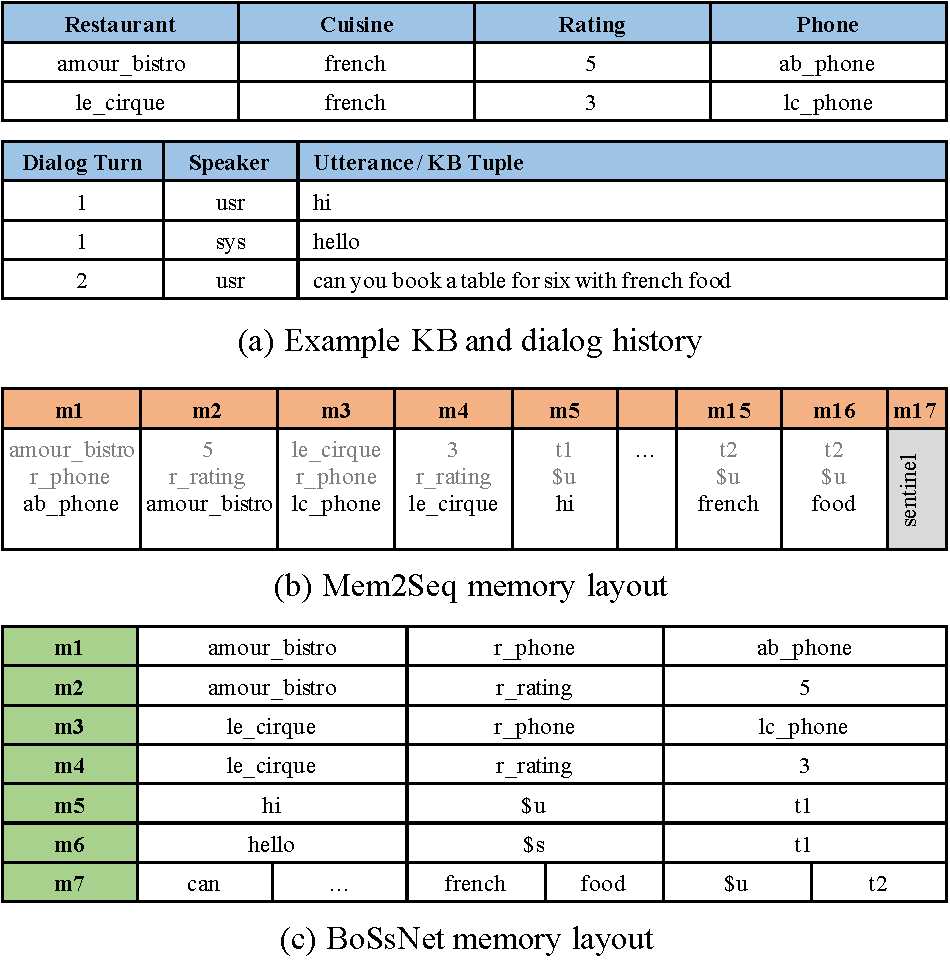
\includegraphics[scale=0.8]{assets/figures/mem2seq.pdf}
\caption{(a) an example dialog with history and KB tuples. (b) an illustration of Mem2Seq memory. (c) an illustration of \sys\ memory}
\label{fig:intro}
\end{figure}

%Our model has the following differences when compared to Mem2Seq: 1) The memory in Mem2Seq has a flat representation whereas we propose a hierarchical representation. 2) The performance of Mem2Seq is dependent on the ordering of KB tuples (subject or object), while the performance of \sys\ is independent of any such ordering. 

% Describe the memory layout
% Each memory element contains either a KB tuple or a word from an utterance in the dialog history. For example, 

% Describe problem #1 and #2
First, Mem2Seq expects each tuple to be serialized by the KB API in way that the object always comes last. This may or may not always be in control of the neural model. Second, because each utterance word has a unique memory cell. it loses the context in which the word was mentioned. As a result, the model cannot learn that ``french'' and other cuisines are usually followed by the word ``food''. This causes poor generalization where the model has to understand an OOV word from the user utterance (e.g., a new cuisine or city name). 
% The vector representation of each memory element is computed using a bag-of-words model. Thus the memory structure prevents the model to generalize by learning clues from the context. 

% Describe problem #3
Finally, the model design dictates that the subject or the predicate from a KB fact can never be copied during the decode step. This adds severe limitations in practical settings. For example, the KB results in the original bAbI dataset \cite{BordesW16} came in format of {\em attribute(restaurant\_name, restaurant\_attribute)}. Since restaurant name is never an object, Mem2Seq would never be able to copy it when making recommendations. As a result, experiments with Mem2Seq necessitated a training data preprocessing, in which all rating facts had to be inverted into {\em rating(restaurant\_rating, restaurant\_name)}, so that the name could become an object and could be copied. 

We believe that this adds severe limitations on the scenarios in which Mem2Seq is applicable. We perform several experiments on the original (unprocessed) datasets to highlight the loss in performance due to these modeling choices. 
In contrast, \sys\ uses a hierarchical memory that can copy {\em any} word from the whole dialog history (see Figure \ref{fig:intro}(c)). It models each cell as a {\em sequence} of words, which also enables it to learn contextual cues for each word, leading to better OOV generalization. 

%The designer needs to carefully choose how a tuple should be placed in the memory. In the example, the object of \textit{r\_phone} (placed at the bottom) is chosen to be the word to copy, while the subject is chosen for \textit{r\_rating}. The placement is dictated by what needs to be copied while generating the response. In the experiments, how ordering affects its performance.

%In the dialog bAbI dataset \cite{BordesW16}, the name of the restaurant and the phone numbers are needed to be copied. Mem2Seq will not be able to generate a response such as ``amour_bistro has a rating of 5'' as the rating object is not addressable by the copy mechanism. 

%Also, if a word occurs more than once in the memory, only the last occurrence of the word is used for computing the copy distribution. This makes the system depend on the order in which KB tuples are placed in the memory
%\todo{Does it fit better now ?}

\section{Components Survey}

\sys\ architecture has a {\em multi-hop encoder}, and a {\em pointer network} decoder with a {\em hierarchical attention} over the memory. The extended architecture has an {\em RL-based API decoder} with mixed on-policy and off-policy sampling. We briefly survey these strands of related research.

\vspace{0.5ex}
\noindent
\textbf{Multi-hop Networks} reason over a sequence of sentences fed as input. A hop refers to reading the sentences and generating a encoded-vector. Multi-hop refers to making multiple updates to the encoded-vector by iteratively reading the input. End to end memory network (MN) \cite{sukhbaatar2015end} represents the input as a set of sentences. Here the encoded-vector is updated by adding iterative reads.~Query reduction network \cite{seo2016query} reads the sentences sequentially using an RNN like unit called the QRN unit. Dynamic memory network \cite{kumar2016ask} also reads the sentences sequentially, and also updates the encoded-vector using a recurrent cell. Gated memory network \cite{liu2017gated} uses a gating mechanism to update the encoded-vector. %Our network also falls under this family of networks.

MN \cite{BordesW16}, gated MN and QRN have been used to learn task-oriented dialogues. \sys\ has two key differences from such architectures. First, existing models select a response from a predefined list of candidates (retrieval model), whereas \sys\ has a decoder that generates the response one word at a time. Second, the memory in \sys\ is hierarchical, i.e., each memory element is a sequence of words vectors rather than just a single utterance vector. This enables the generator to copy any word from the memory during generation.

%The two main differences such approaches and our approach are: (1) these model select a response from a predefined list of candidates where as our approach generates responses. (2) The memory is hierarchical (i.e.,) each memory element is a sequence of words rather than just a vector. This enables the generator to copy any word from the memory during generation.

\vspace{0.5ex}
\noindent\textbf{Pointer Networks} are sequence to sequence (Seq2Seq) models, where each token in the output sequence corresponds to a token at a certain position in the input sequence \cite{vinyals2015pointer}. By enabling pointing in Seq2Seq models \cite{cho2014learning,sutskever2014sequence}, the effective decode vocabulary becomes the union of the fixed decode vocabulary and the vocabulary of the input sequence. Two main methods \cite{gu2016incorporating,eric2017copy} exist for incorporating pointing in standard Seq2Seq models -- hard decision \cite{nallapati2016abstractive,gu2016incorporating,eric2017copy} and soft switch \cite{see2017get}. The former makes a hard choice between using the pointer distribution and the decode vocabulary distribution. It usually requires the hard decision to be labeled. The latter approach learns a soft interpolation between the two distributions without explicit labels. \sys\ employs a soft switch in its decoder.

%\cite{see2017get} combined the pointer distribution and the decode vocabulary distribution using a soft switch, where as \cite{nallapati2016abstractive} used either the pointer distribution or the decode vocabulary distribution based on a hard decision. The former learns the soft switch latently without explicit labels, while the latter requires the hard decision to be labeled. Since, we wish the system to automatically learn when to generate and when to point, we use an approach similar to one proposed in \cite{see2017get}.

Eric and Manning
\cite{eric2017copy} use a copy augmented Seq2seq model for learning task-oriented dialogues. This approach uses a hard decision to pick between the generate and pointer distributions. This model is explicitly trained to only point to words that are from the KB and generate the rest. This is the closest work to our approach, but has a flat memory and doesn't incorporate multi-hop reasoning.

\vspace{0.5ex}
\noindent\textbf{Hierarchical Attention} was first introduced for document classification \cite{yang2016hierarchical}. Here, each document is represented as a set of sentences and each sentence as a set of words. For each sentence, an attention distribution is computed over words to identify informative words and compute a sentence representation. A similar approach identifies informative sentences to compute a document representation. Hierarchical attention has also been used for abstractive text summarization \cite{nallapati2016abstractive}.
\sys\ similarly computes two attention distributions over different levels of the input. A word-level distribution over the words in each utterance and an utterance-level distribution over all the input utterances. This a function of these two distributions is used when copying a word in the decode process.

\vspace{0.5ex}
\noindent\textbf{Reinforcement Learning} has been coupled with Seq2Seq architechures to solve tasks like program induction \cite{liang2017neural, zaremba2015reinforcement}, SQL query generation \cite{NIPS2018_8204, zhong2017seq2sql}, and dialog generation \cite{li2016deep}. These systems generate output responses which are associated with a final reward. The REINFORCE \cite{williams1992simple} algorithm is used to train such systems from weak supervision and directly maximize the expected reward. Since learning from scratch is difficult for REINFORCE, it is augmented with an iterative maximum likelihood (ML) training process \cite{liang2017neural}. Memory Augmented Policy Optimization (MAPO) \cite{NIPS2018_8204}, leverages a memory buffer of promising trajectories to reduce the variance of policy gradient estimate. It uses distributed sampling from inside and outside of the memory buffer to scale up training.

\sys -RL leverages these techniques to generate a valid API call to the Knowledge Base. However, it differs from the other methods as the decoder has to train using implicit reward which depends on the final system responses based on the KB results queried by the predicted API.

\section{Preliminaries}
\label{sec:prelims}
In this section, we briefly describe the preliminaries over which the proposed \sys\ architecture is built upon as explained in the previous section. This includes (1) the multi-hop encoder in MN and (2) a standard sequence decoder with attention \cite{bahdanau2014neural}

\noindent\textbf{Multi-Hop Encoder in MN}
\label{ssec:mhencoder}

The multi-hop encoder as described in end-to-end memory network \cite{sukhbaatar2015end} takes as input a query $q \in \mathbb{R}^{d}$ and a memory $M = \{ m_i; m_i \in \mathbb{R}^{d}\}$ and generates a reduced query $q_r \in \mathbb{R}^{d}$. Here $d$ is the embedding dimension. Augmenting the query by attending it over the memory elements, to capture relevant information necessary to generate the response, is referred to as a \textit{hop}. A single hop reduced query is computed as follows:
\begin{eqnarray}
p_i &=& \text{softmax}(q^T m_i) \\
o &=& W_r \sum\nolimits_i p_i m_i \\
q_r &=& o + q
\end{eqnarray}
where $W_r \in \mathbb{R}^{d \times d}$. The hop step can be re-iterated, by assigning the output of the previous hop as the new input query (i.e.,) $q=q_r$. If the encoder has $K$ hops, then the final output is represented as $q^k_r$. The multiple hops enable inference over multiple memory elements.

\noindent\textbf{Sequence Decoder with Attention}
\label{ssec:rnndecoder}

The sequence decoder predicts the token $y_t$ in the output sequence $\langle y_1 y_2 \ldots y_T \rangle$, given the decoder state at time $t$, $s_t$, and a set of input contexts $Z=\{z_i ; z_i \in \mathbb{R}^{d}\}$. For simplicity, we denote this conditional distribution of generating the next word as just $P_g(y_t)$. To compute $P_g(y_t)$, first an attention distribution $\alpha^t$ is computed over the input contexts $z_i$ using Loung attention \cite{luong2015effective}. 
\begin{gather}
u_i^t = s_t W_l z_i \\
\alpha_i^t = \frac{exp(u_i^t)}{\sum\nolimits_{k}exp(z_k^t)} \label{eq:memattn}
\end{gather}
where $W_l \in \mathbb{R}^{d \times d}$. Then, a context vector $z^*_t$ is generated by performing a weighed sum of the input contexts $z_i$ using the attention distribution $\alpha^t_i$.
\begin{comment}
\begin{gather}
z^*_t = \sum\nolimits_i \alpha^t_i z_i 
\end{gather}
\end{comment}
The context vector concatenated with the decoder state $s_t$ is then used to compute the \textit{generate distribution} over the decode vocabulary $\mathcal{V}$ at time $t$ as follows:
\begin{gather}
P_{g}(y_t)= \text{softmax}( W_d [s_t;z^*_t] + b )
\end{gather}
where $W_d \in \mathbb{R}^{|\mathcal{V}| \times 2d}$ and $b \in \mathbb{R}^{|\mathcal{V}|}$ are parameters to be learnt. $[;]$ indicates vector concatenation along the row.

During training, the objective is to minimize the average negative log-likelihood for all the words in the response.
\begin{comment}
\begin{gather}
\mathcal{L}=-\frac{1}{T}\sum\nolimits_{t=1}^{T}log P_{g}(y_t)
\label{eq:loss}
\end{gather}
\end{comment}
The total loss is computed by adding the loss of all the responses in the training data.

\noindent\textbf{Augmented REINFORCE}
\label{ssec:Areinforce}

Lets consider the setting where given a query $x$, the state, action and reward at each time step $t \in {0, 1, \dots, T }$ are ($s_t$, $a_t$, $r_t$). In a deterministic environment the state is defined by the query $x$ and the action sequence: $s_t = (x, a_{0:t-1})$, where $a_{0:t-1} = (a_0, \dots, a_{t-1})$ is the history of actions at time $t$. If the reward at time $t$ is given by $r_t$, then the cumulative reward of a action sequence $a_{0:T}$ is defined as:
\begin{gather}
R(x, a_{0:T}) = \sum_{t}r_t
\end{gather}
The agent’s decision making procedure at each time is defined by a deterministic policy, $\pi_\theta(s,a) = P_\theta(a_t = a|x, a_{0:t-1})$, where $\theta$ are the model parameters. The probability of generating a sequence $a_{0:T}$ is:
\begin{gather}
P_\theta(a_{0:T}|x) = \prod_{t}P_\theta(a_t|x, a_{0:t-1})
\end{gather}
We can define our objective to be the expected cumulative reward and use policy gradient methods such as REINFORCE for training. The objective and gradient are:
\begin{gather}
J^{RL}(\theta) = \sum_{x}\mathbb{E}_{P_\theta(a_{0:T}|x)}[R(x, a_{0:T})] \\
\nabla_\theta J^{RL}(\theta) = \sum_{x}\sum_{a_{0:T}}P_\theta(a_{0:T}|x)\cdot[R(x, a_{0:T}) - B(x)]\cdot\nabla_\theta \log P_\theta(a_{0:T}|x)
\end{gather}
where $B(x) = \sum\nolimits_{a_{0:T}} P_\theta(a_{0:T} | x)R(x, a_{0:T})$ is a baseline that reduces the variance of the gradient estimation without introducing bias.

Following a similiar pattern to imitaion learning \cite{ross2011reduction, berant2015imitation} we can calculate a $a^{best}_{0:T}$ based on maximum likelihood and add them to the set of action sequences with a resonably large probability. We define a parameter $\alpha$ and with each iteration, we scale the probabilities of the on-policy action sequences by $(1 - \alpha)$ and then add the calculated $a^{best}_{0:T}$ with a probablity $\alpha$. This augmented REINFORCE leads to faster convergence and stabilises training.
\pagebreak

%%%%%%%%%%%%%%%%%%%%%%%%%%%%%%%%%%%%%%%%%%%%%%%%%%%%%%%%%%%%%%%%%%%%%%
% Approach
\chapter{APPROACH}
\label{chap:approach}
% Summary of what we are about to describe
In this chapter, we first describe the {\sc BoSs} memory which contains the dialog history and KB tuples, followed by how the memory is consumed by the encoder and the decoder. We then define the loss function, which, along with dropout, enables disentangled learning of language and knowledge. Finally we go on to explain the RL-decoder and its integration in the \sys -RL architecture.

\section{The \sys\ Architecture}
% Quick Intro
The proposed Bag-of-Sequences Memory Network has an encoder-decoder architecture that takes as input (1) dialog history, which includes a sequence of previous user utterances $\{c_1^u, \ldots, c_{n}^u\}$ and system responses $\{c_1^s, \ldots, c_{n-1}^s\}$, and (2) KB tuples $\{kb_1, \ldots, kb_{N}\}$. The network then generates the next system response $c_n^s=\langle y_1 y_2 \ldots y_T \rangle$ word-by-word. The simplified architecture of \sys\ is shown in Figure \ref{fig:simsystem} and a more detailed architecture is shown in \ref{fig:fullsystem}.
%The network maintains the dialog history and KB tuples in the {\em Bag-Of-Sequences memory}.
% Notations Used

\begin{figure}[t]
\centering
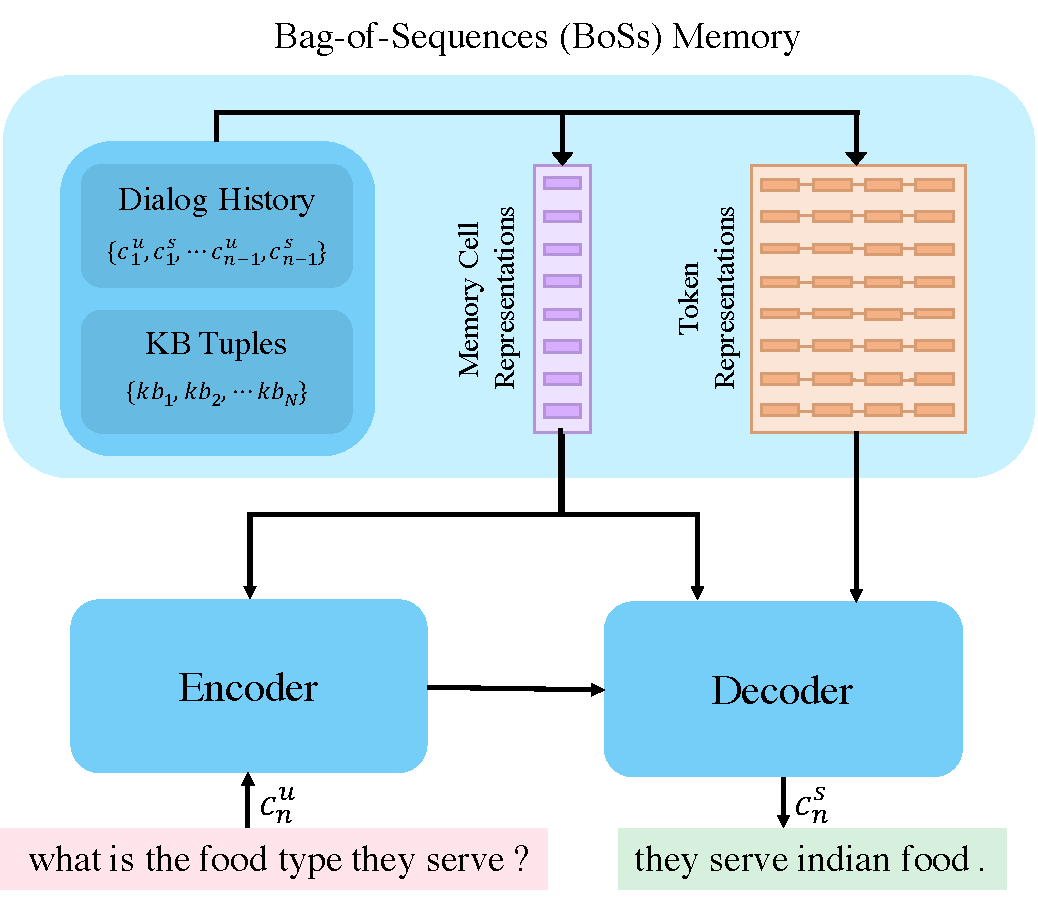
\includegraphics[scale=0.5]{assets/paper_arch.pdf}
\caption{The dialog history and KB tuples stored in the memory have memory cell representations and token representations. The encoder understands the last user utterance using only the memory cell representations. The decoder generates the next response using both representations.}
\label{fig:simsystem}
\end{figure}

\begin{figure}
\centering
\begin{subfigure}{0.8\textwidth}
 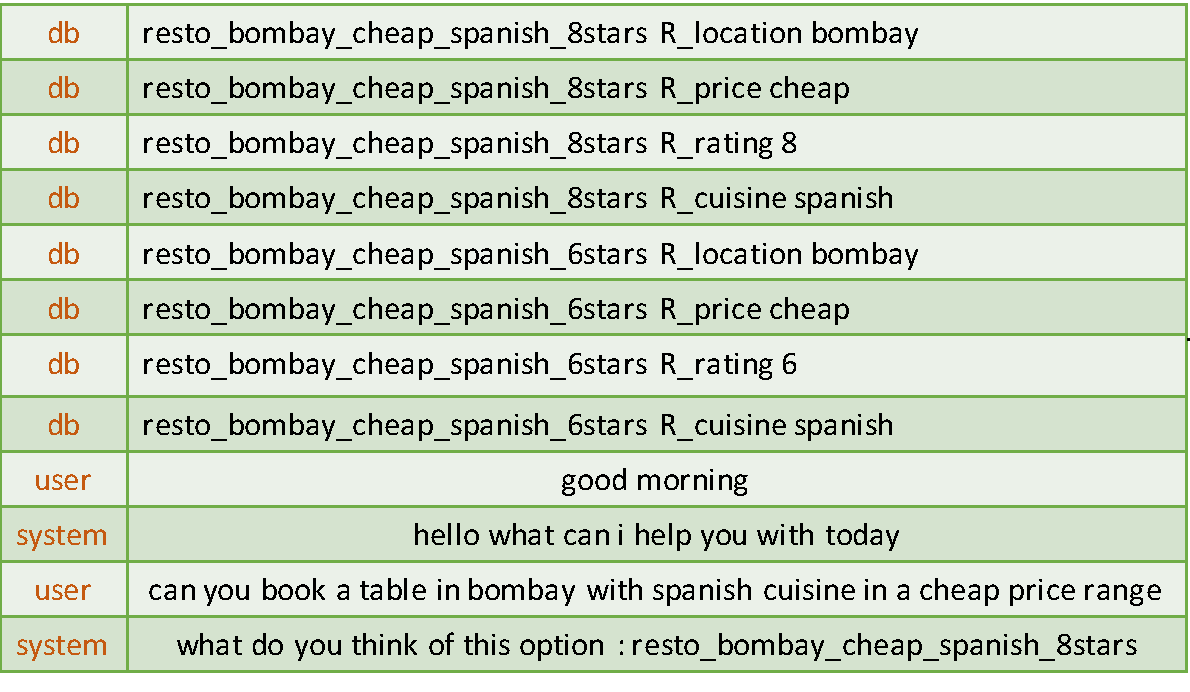
\includegraphics[width=\linewidth]{assets/figures/memory_flat.pdf}
 \caption{Simple Memory Representation (Sentence Level)}\label{fig:flatMemory}
\end{subfigure}

\vspace*{0.5in}

\begin{subfigure}{0.8\textwidth}
 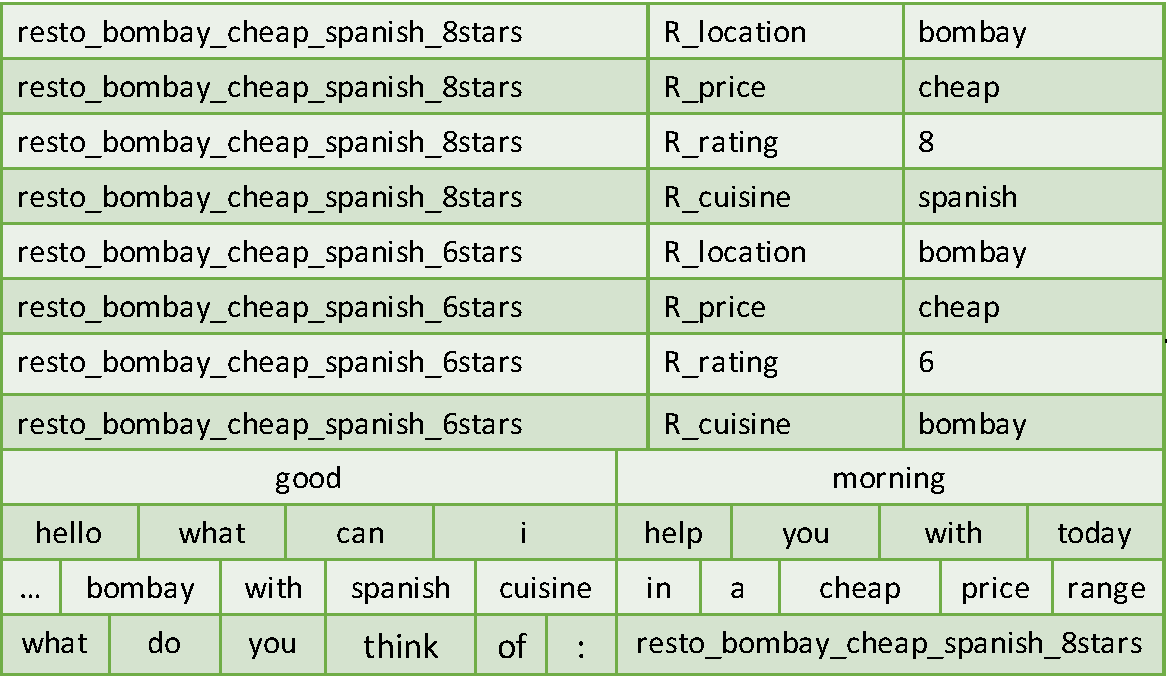
\includegraphics[width=\linewidth]{assets/figures/memory_hier.pdf}
 \caption{{\sc BoSs} Memory Representation (Sentence + Word Level)}\label{fig:hierMemory}
\end{subfigure}
\caption{Types of Memory Architectures}
\end{figure}

\begin{figure}[t]
\centering
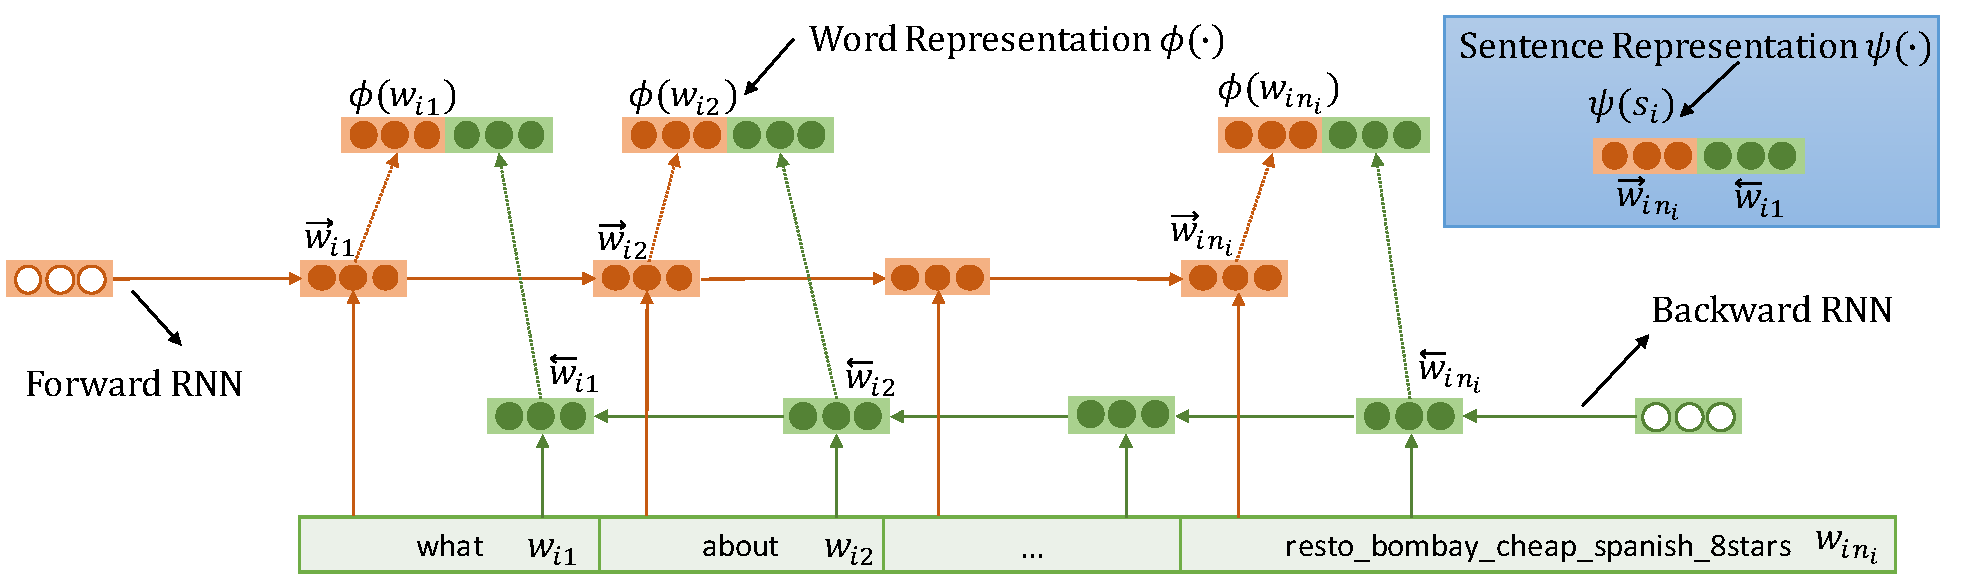
\includegraphics[scale=0.5]{assets/figures/embedding.pdf}
\caption{Each sentence is passed through a bi-directional GRU. We obtain word level embeddings $\phi(w_i)$ and sentence level embeddings $\psi(s_i)$ by concatinating the result of the front and back passes.}
\label{fig:embed}
\end{figure}

\subsection{Bag-of-Sequences Memory} 
\label{sec:hmemory}
The context memory $M$ contains the dialog history $\{c_1^u, c_1^s, \ldots, c_{n-1}^u, c_{n-1}^s\}$ and the KB tuples $\{kb_1, \ldots, kb_{N}\}$. Each utterance in the dialog history and each KB tuple is placed in a memory cell as seen in Figure \ref{fig:hierMemory}. As utterances and tuples are inherently a sequence, we represent each memory cell $m_i$ as an ordered sequence of tokens $\langle w^1_i w^2_i \ldots w^{|m_i|}_i\rangle$. For an utterance, the word tokens are followed by a temporal indicator and a speaker indicator \{\$u (for user), \$s (for system)\}. For example, \{\texttt{good, morning, \#1, \$s}\}\ indicates this was the first utterance by the system. For a KB tuple, the tokens are sequenced as \{\textit{subject, predicate, object}\} followed by temporal indicator and a kb indicator (\texttt{\$db}).

Token representation is generated using a bidirectional GRU. Let the outputs of the forward and backward GRUs for the token $w^j_i$ be denoted as $\overrightarrow{h^j_{i}}$ and $\overleftarrow{h^j_{i}}$ respectively. Then the token representation $\phi(w^j_i)$ is given by Eq. \ref{eqn:1}. Memory cell representation $\psi(m_i)$ is computed by concatenating the forward GRU output of its last token and the backward GRU output of its first token as in Eq. \ref{eqn:2}. This is further visualised in Figure \ref{fig:embed}
\begin{eqnarray}
\phi(w^j_i)=[\overrightarrow{h^j_{i}};\overleftarrow{h_{i}^j}] \label{eqn:1} \\
\psi(m_i)=[\overrightarrow{h_{i}^{|m_i|}};\overleftarrow{h_{i}^1}] \label{eqn:2}
\end{eqnarray}

\begin{figure}[t]
\centering
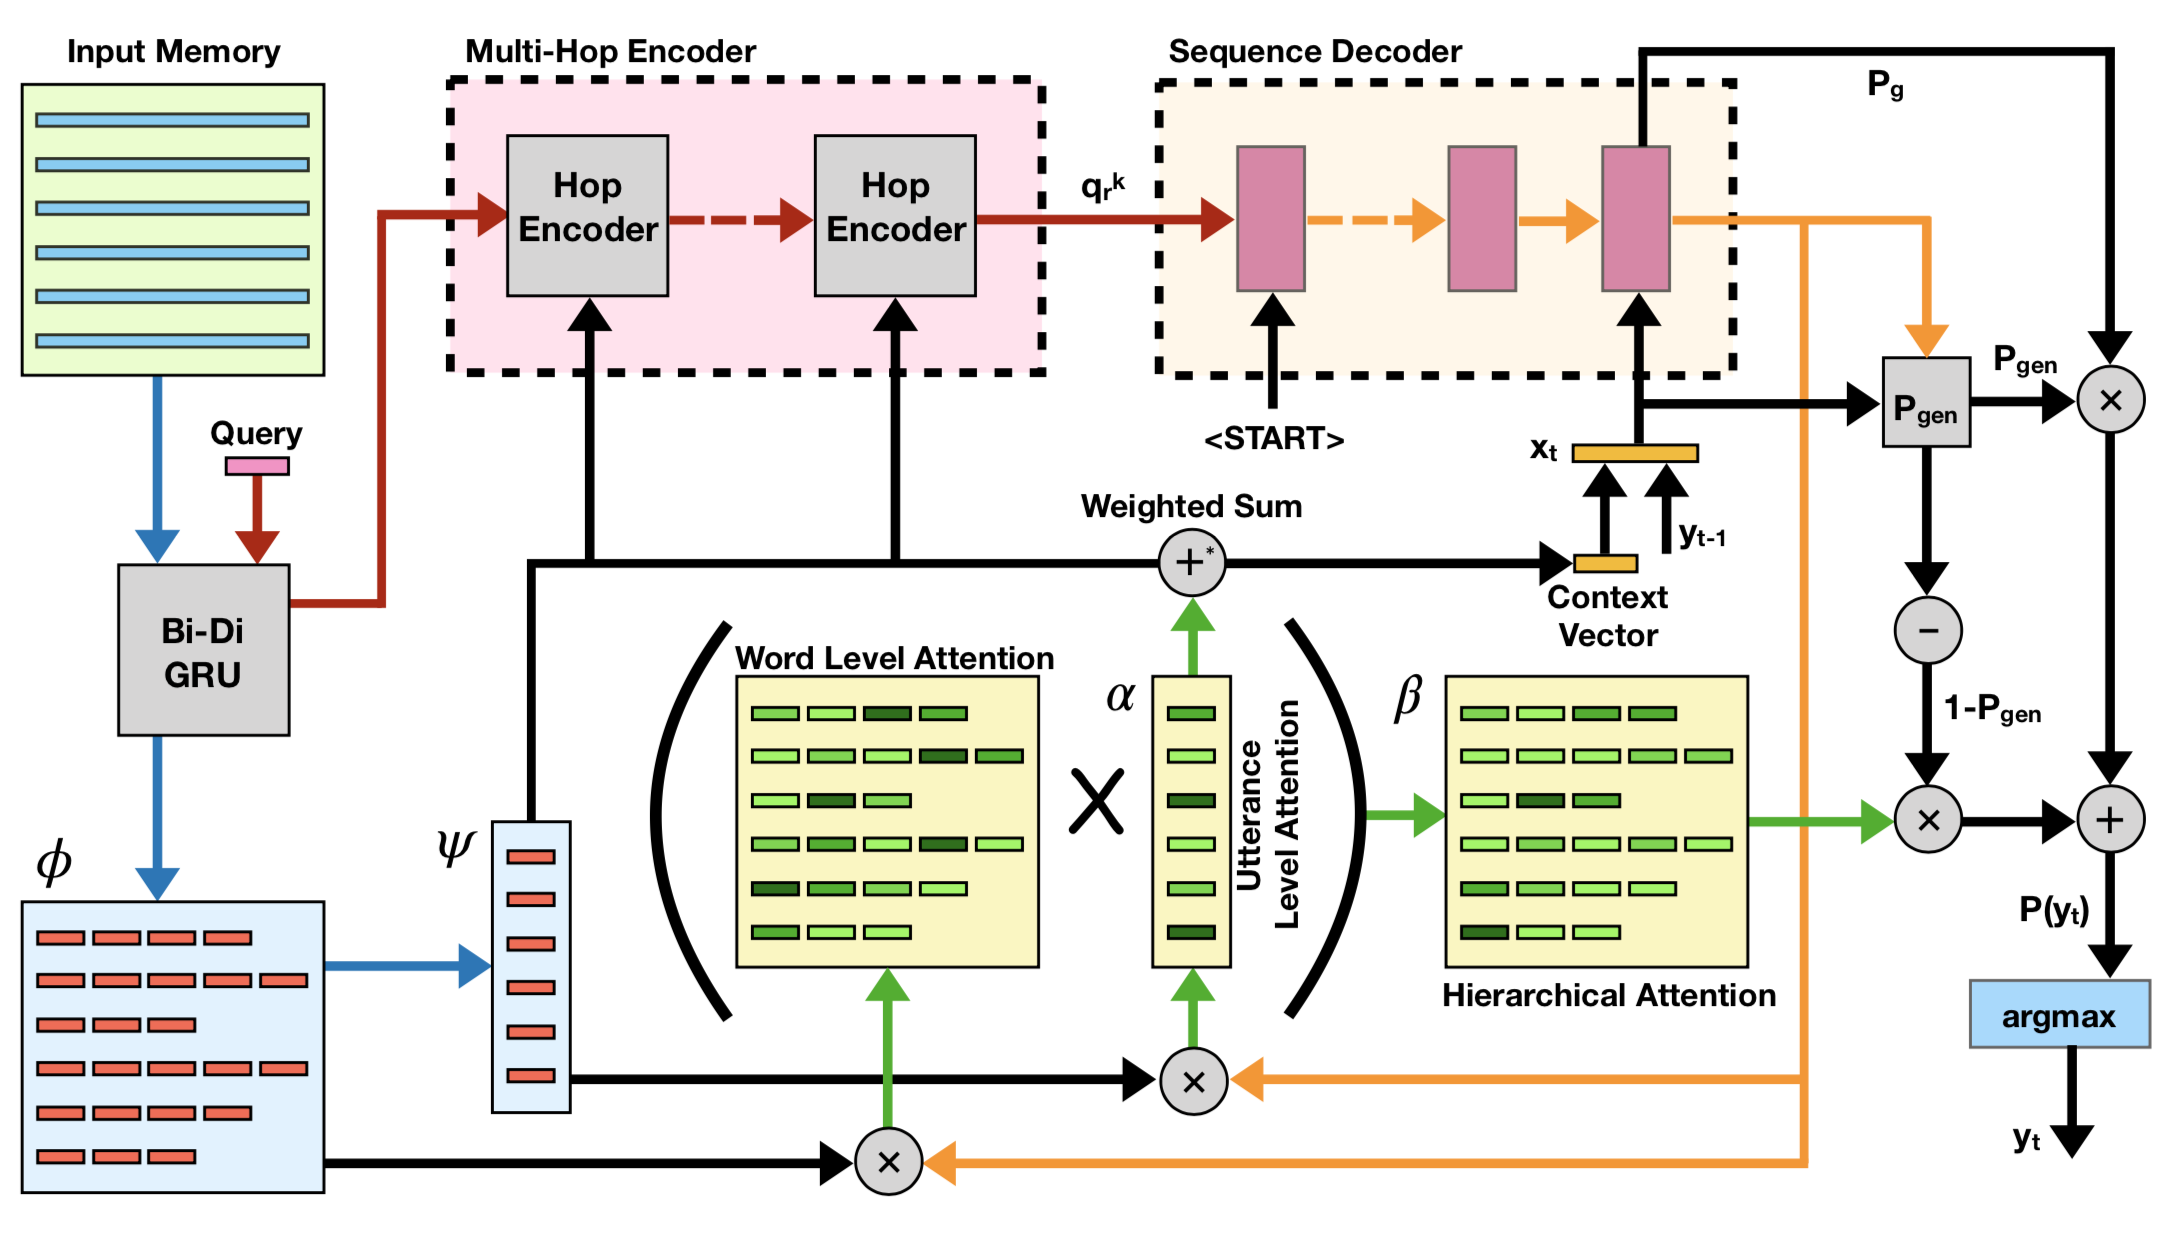
\includegraphics[scale=0.4]{assets/paper_arch.png}
\caption{The detailed encoder-decoder architecture of \sys\ depicting attention over its hierarchical memory and implementation of its copy mechanism.}
\label{fig:fullsystem}
\end{figure}

%\textcolor{blue}{The encoder uses only the memory cell representations to summarize the dialog history and the KB, while the decoder peaks at both the memory cell representation and the token representations during each decode step.}\todo{[N: This is unclear]}

\subsection{The \sys\ Encoder}
\label{ssec:encoder}

The encoder used in \sys\ is similar to the multi-hop attention encoder with layer-wise weights proposed by \cite{sukhbaatar2015end}. The encoder in \cite{sukhbaatar2015end} uses two different embedding matrices, whereas we use just one to reduce the number of parameters. The encoder considers the last user utterance as the query $q=\psi(c_n^u)$ and computes the reduced representation $q_r$ using the memory $M$ as follows:
\begin{eqnarray}
p_i &=& \text{softmax}(q^T \psi(m_i)) \\
o &=& W_r \sum\nolimits_i p_i \psi(m_i) \\
q_r &=& o + W_o q
\end{eqnarray}

where $W_r, W_o \in \mathbb{R}^{d \times d}$ are learnable parameters. The hop step can be re-iterated, by assigning the output of the previous hop as the new input query, i.e., setting $q=q_r$. The output of the encoder after $K$ hops, $q_r^k$, is assigned as the initial state of the decoder.

\subsection{The \sys\ Decoder}
\label{ssec:decoder}

\sys\ models a copy-augmented sequence decoder, which generates the response one word at a time. At any decode time step $t$, the decoder can either \emph{generate} a word from the decode vocabulary or \emph{copy} a word from the memory. Consequently, the decoder computes: (1) generate distribution $P_g(y_t)$ over the decode vocabulary, and (2) copy distribution $P_c(y_t)$ over words in the memory. 

The generate distribution is computed using a standard sequence decoder \cite{sutskever2014sequence} by attending \cite{luong2015effective} over the memory cell representations $\psi$. The copy distribution is generated by using a \textit{two-level attention} over the {\sc BoSs} memory. Given the decoder state $s_t$, it first computes attention $\alpha_t$ over the memory cells. Then it computes attention over the tokens in each memory cell $m_i$. Finally it multiplies both these attentions to compute $P_c(y_t)$ as follows: 
\begin{gather}
\alpha_i^t = \text{softmax}(s_t \psi(m_i)) \\
e_{ij}^t = s_t \phi(w_i^j) \\
\beta^{t}_{ij} = \alpha^t_i * \frac{\exp({e_{ij}^t})}{\sum\nolimits_{k}\exp({e_{ik}^t})} \\
%\beta^{t}_{ij} = \alpha^t_i * \sigma(e_{ij}^{t}) \\
P_c(y_t=w)=\sum_{ij:w_i^j=w} \beta_{ij}^{t}
\end{gather}

%\textcolor{blue}{where $W^w_l, W^u_l \in \mathbb{R}^{d \times d}$ are learnable parameters.}
%\todo{[N: I think we dont use the weight matricies for attention due to extra parameters and low performance.]}

The copy and generate distributions are combined using a soft gate $g_s^t \in [0,1]$ as in \cite{see2017get}. $g_s^t$ is a function of the decoder state at time $t$ and the previous decoded word $y_{t-1}$.
\begin{gather}
g_s^t = W_g[s_t;y_{t-1}] + b \\
P(y_t) = g_s^{t}P_g(y_t) + (1-g_s^{t})P_c(y_t)
\end{gather}


\subsection{Loss}
The decoder is trained using cross-entropy loss. The loss per response is defined as:
\begin{equation}
\mathcal{L}_{ce} = - \sum_{t=1}^{T} \textup{log} \Big( g_s^{t}P_g(y_t) + (1-g_s^{t})P_c(y_t) \Big) 
%\\ + \gamma \sum_{t=1}^{T}H(p^{(t)}_{gen}, p^{(t)}_{ref-gen}) 
\end{equation}
where $T$ is the number of words in the sequence to be generated and $y_t$ is the word to be generated at time step $t$. The decision to generate or copy is learnt implicitly by the network. However, to attain perfect disentanglement, the KB words should be copied, while the language should be generated. In other words, any word in the response that is present in the {\sc BoSs} KB memory should have a low $g_s$. To obtain this behavior, we define a disentangle label $D_{l}$ for each word in the response. This label is set to $1$ if the word is present in the {\sc BoSs} KB memory and $0$ otherwise.
We define a disentangle loss as follows:
\begin{equation}
\mathcal{L}_{d} = - \sum_{t=1}^{T} g_s^{t}\textup{log}D^{t}_{l} + (1-g_s^{t})\textup{log}(1-D^{t}_{l})
\end{equation}

We randomly drop some words with disentangle label set to $1$. This \textit{Disentangle Label Dropout (DLD)} works in tandem with the disentangle loss and {\sc BoSs} memory -- it encourages the model to copy KB words whenever possible, based on their surrounding words. The overall loss is given as:
\begin{equation}
\mathcal{L} = \mathcal{L}_{ce} + \gamma \mathcal{L}_{d}
\label{eqn:loss}
\end{equation}

The relative weight of $\mathcal{L}_{d}$ in the overall loss is controlled using a hyper-parameter ($\gamma$). The dropout rate is also a hyper-parameter.

\section{The \sys -RL Architecture}
The reinforment learning based API generation system builds upon the original \sys\ architecture with the following modules: (1) API Explorer, (2) RL-decoder, and (3) Augmented REINFORCE. We explain these in the upcoming sections.

\subsection{API Explorer}
This module has the objective of aiding the exploration of valid APIs with a strong reward. Our actual reward for a generated API is implicit, because it depends on the responses of the response model based on the results queried by the API. Hence, we go on to define a psuedo reward for each API as the following:

\noindent\textbf{Psudo Reward}
\label{ssec:PsReward}
The responses by the system depend on the results fetched by the API from the KB. The system will only be able to copy KB information into its response limited to these results. Hence we can measure the performance of a certain API by checking the overlap of the information required by the responses and that present in its results. We use the popular F1 metric which is a combination of precision and recall. For us recall is important because it measures the extent of overlap and the precision will make sure that the results retrieved say as concise as possible. We don't want to have a very generic API which results in a very large result set!. Our metric which we term as the {\em Psuedo Reward} is calculated as follows.
\begin{gather}
Reward = \frac{2 \cdot R \cdot P}{(R + P)}
\end{gather}
where $P$ = No. of KB items in both results and responses / No. of KB items in results \\ and $R$ = No. of KB items in both results and responses / No. of KB items in responses

Our API Explorer then tries to find (explore) valid APIs/queries with a large psuedo-reward to aid in augmented REINFORCE explained in the sections below.

\subsection{RL-decoder}
\label{ssec:rldecode}
The RL-decoder is added as a second decoder to the \sys\ architecture, and is only activated when the system receives a {\em Make API} command. It uses a different embedding matrix from the original encoder to encode the context which serves as the initial state to the decoder. The decoder uses a sequence independence approach to generate the output akin to a slot-filling technique with a fixed template as shown in Figure \ref{fig:rldec}. Since the API has been templated it will always generate the same length trajectory and hence it mitigates the length bias issue. Also since each slot is being predicted independent of each other, the decoder will attempt to pick up as much informatiom as possible each time. This will mitigate the data bias issue which arises from the ability to choose what parameters to send in the API call, whereas we generally want to be as precisise as possible.

The initial state is passed on at each timestep of the decode process and only the current timestep is given as input, as in Eq. \ref{eqn:dec}. This makes each decode step independent of the previously decoded sequence and it is completely focused on finding the correct information in the context to fill in its current slot/timestep. The decoder is implemented using beam-search and employs constraint decoding over a fixed grammar/template.
\begin{eqnarray}
s_{t} = W_d [s;p_t] + b \label{eqn:dec}
\end{eqnarray}
where $s$ is the initital state to the decoder and $p_t$ is the position embedding for the current time step.

\begin{figure}[!t]
\centering
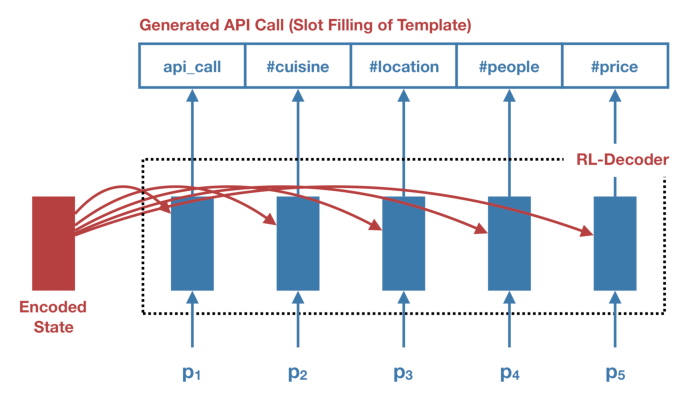
\includegraphics[scale=1.1]{assets/figures/rl_decoder.pdf}
\caption{The decoder attempts to fill a predefined template of fixed length. It uses only the encoded state and current position $p_t$ to decode to maintain independence between slots.}
\label{fig:rldec}
\end{figure}

\subsection{Augmented REINFORCE}
% At each iteration our RL-decoder creates several on-policy predictions using beam search decoding. Each one has its own associated probability and is assigned a psuedo-reward. 
The API explorer maintains a buffer of size $M$ containing the set of promising APIs, denoted by $\mathcal{B} = \bigl\{a^{(i)}\bigr\}_{i=1}^M$, where $a \in \mathcal{A}$ is a valid API trajectory in our entire space of possible trajectories $\mathcal{A}$. We modify our expected objective of our policy $\pi_\theta$, as done in \cite{NIPS2018_8204}, as a weighted sum of two terms: an expectation over the trajectories inside the memory buffer, and a separate expectation over the trajectories outside the buffer.

\begin{gather}
J^{RL}(\theta) = \alpha\sum_{a\in\mathcal{B}}\pi^+_\theta(a)R(a) + (1-\alpha)\sum_{a\in(\mathcal{A}-\mathcal{B})}\pi^-_\theta(a)R(a) 
\end{gather}

here $\pi^+_\theta$ and $\pi^-_\theta$ denote the normalised probablity in and outside the buffer respectively.

\begin{gather}
\pi^+_\theta(a) = \begin{cases}
             \pi_\theta(a) / \alpha  & \text{if } a \in \mathcal{B} \\
             0  & \text{if } a \notin \mathcal{B}
       \end{cases}, \quad
\pi^-_\theta(a) = \begin{cases}
             0  & \text{if } a \in \mathcal{B} \\
             \pi_\theta(a) / (1-\alpha)  & \text{if } a \notin \mathcal{B}
       \end{cases}
\end{gather}

The first term of the expectation can be calculated over the entire buffer which is typically small in size. The second expection requires us to sample from $\pi_\theta$, using beam search over our RL-decoder, and then employing rejection sampling w.r.t the examples in the buffer. This will ensure that the buffer and our on-policy samples are mutually exculsive. The entire pipeline is visualised in Figure \ref{fig:rlupdate}.

\noindent\textbf{Dealing with Language Bias}
Several default inputs such as {\em dontcare} or {\em null} occur very frequenntly in valid APIs. As a result the policy is biased to pick them on occasion. We attempt to mitigate this issue by dividing our dialogs into two sets: (1) confident and (2) confused. The confident examples are the dialogs with no null slots. Confused dialogs on the other hand have one or more null slots and hence multiple APIs giving the best set of results. The confident examples are trained in a similar setting to supervised learning by keeping only the one best API in the buffer. This leads to a robust system and it helps bias it to learn the confused examples correctly.

\begin{figure}
\centering
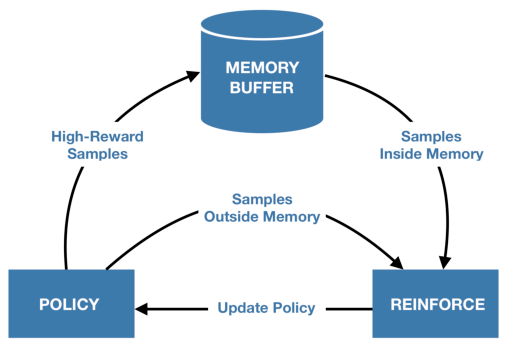
\includegraphics[scale=1.0]{assets/figures/rl_update.pdf}
\caption{The policy update algorithm. A mix of on and off-policy samples are used to train the policy and any new promising trajectories are added to the buffer.}
\label{fig:rlupdate}
\end{figure}

\pagebreak

%%%%%%%%%%%%%%%%%%%%%%%%%%%%%%%%%%%%%%%%%%%%%%%%%%%%%%%%%%%%%%%%%%%%%%
% Implementation
\chapter{IMPLEMENTATION}
\label{chap:implementation}
In this chapter we will discuss the implementation on various modules of the \sys\ architecture. We start off by describing all the components we worked on and then explain in detail the parts which are relevant to this thesis.

\section{Parts of the \sys\ Architecture}

We have created multiple modules, each with a different functionality and objective. We list the major modules in the \sys\ architecture below:

\begin{enumerate}
	\item \textbf{Main Controller} - This component manages the flow of data and information among the other components. It reads and cleans the data and manages the training and prediction of the dialogs via the memory network.
	\item \textbf{Data Loader} - This is incharge of reading all the data from files and formatting it in an easy to use way.
	\item \textbf{Data Batcher} - This module takes data from the data loader class and performs any preprocessing and indexing required by the Memory network to use the data for training.
	\item \textbf{Memory Network} - This is the network of the encoder and decoder that both trains and predicts the responses for dialogs given the context and user query.
	\item \textbf{Dynamic Decoder} - This is a built in library of tensorflow that was modified to allow batch decoding and beam search.
	\item \textbf{Attention Mechanism} - This is a built in library of tensorflow that was modified to enable our multi-level attention mechanism.
	\item \textbf{Beam Search} - This is the built in library of tensorflow that was modified to allow constraint decoding and the copy generate mechanism.
	\item \textbf{Evaluator} - This class gives evaluation metric scores on the response predictions by comparing them with the gold examples.
	\item \textbf{Logging} - This component maintains any errors in the code during runtime and allows for automatic deployment of multiple runs. It also generates log files giving detailed explanations of each run.
\end{enumerate}

We depict the interaction between the multiple components in Figure \ref{fig:sys_comp}. Parts in blue have been explained in this thesis. Half colored blocks mean part of the work regarding that component is explained and the rest is not in the scope of this thesis.

\begin{figure}[!ht]
\centering
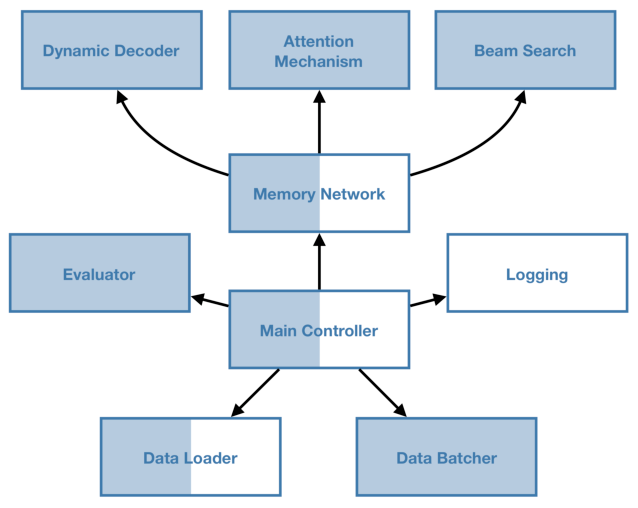
\includegraphics[scale=1.0]{assets/figures/components_orig.pdf}
\caption{Components of the \sys\ system and their interaction.}
\label{fig:sys_comp}
\end{figure}

\noindent\textbf{Main Controller}

\noindent\textbf{Data Loader}

\noindent\textbf{Data Batcher}

\noindent\textbf{Memory Network}

\noindent\textbf{Dynamic Decoder}

\noindent\textbf{Attention Mechanism}

\noindent\textbf{Beam Search}

\noindent\textbf{Evaluator}

\section{Parts of the \sys\-RL Architecture}

There are mainly three main components that have been added to the \sys\ architecture to make \sys -RL. These are listed below.

\begin{enumerate}
	\item \textbf{API Explorer} - This systematically searches the space of APIs and populates the buffer to be used by MAPO.
	\item \textbf{Rewards} - This takes in a particular API as input along with the expected future responses and returns the reward/pseudo-reward.
	\item \textbf{RL-Decoder} - This is the main API generator which we train to learn the ideal policy.
	\item \textbf{Augmented REINFORCE} - This takes in results from both the API explorer populated buffer and the RL-decoder outputs and runs Augmented REINFORCE (MAPO) on top of them.
\end{enumerate}

We observe the interaction between these added components and the previous architecture in Figure \ref{fig:sys_comp_rl}. Below we discuss modifications to previous components and newly added features.

\begin{figure}[t]
\centering
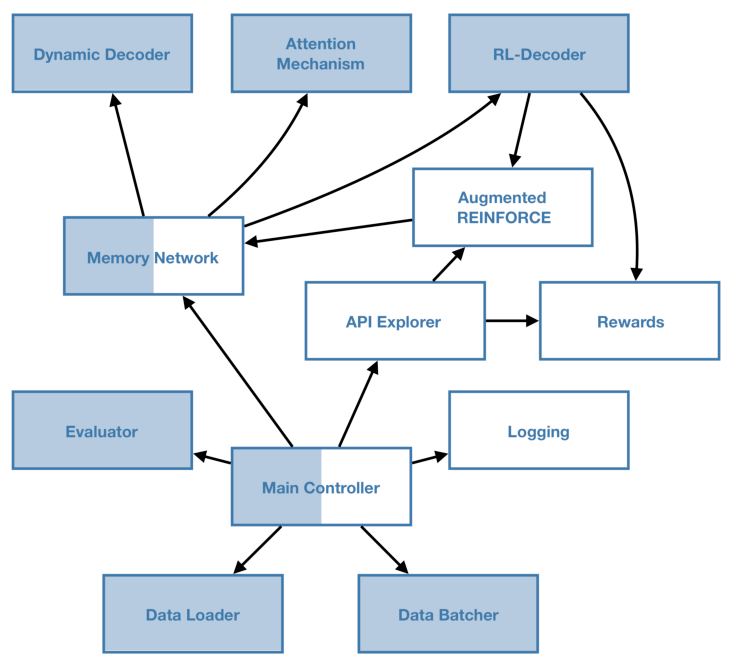
\includegraphics[scale=1.2]{assets/figures/rl_components.pdf}
\caption{The components of the \sys -RL system and their interaction.}
\label{fig:sys_comp_rl}
\end{figure}

\noindent\textbf{Main Controller}

There are several changes that had to be made to the main controller to handle the RL-decoding policy. First, we implemented a phase-wise training to help enable the RL-decoder and the response model to train independently. In this phase we have 4 phases:
\begin{enumerate}
	\item \textbf{Phase 1} : This trains the response deocder only for dialogs that occur before any API is made.
	\item \textbf{Phase 2} : This phase adds in the training for the RL-decoder. This is only used in case we use a shared embedding space for encoding the context for the response deocder and RL-decoder. If they use different embeddings, then Phase 2 can be directly merged with Phase 1.
	\item \textbf{Phase 3} : In this phase we can now start training the system on responses after the API call has been made. We include the results retrieved by the RL-decoder in Phase 2.
	\item \textbf{Phase 4} : This phase calculates the actual reward based on the responses innn Phase 3 and retrains the RL-decoder accordinly. This reward actually measures how well the system was able to train on the retrieved results and will be able to capture the effects of how the results are stored in memory, like sorting based on a field.
\end{enumerate}

These phases are run one after the other and more phases are activated after the previous phases near convergence. For example we start off with just Phase 1 and after it converges we now run Phase 1 and 2 together.

\noindent\textbf{Memory Network}

We added three main APIs in the memory network to enable the RL-decoder. 

\begin{itemize}
	\item \emph{api\_predict} will attempt to predict good API responses via the RL-decoder policy and utilises beam search to get a large set predictions.
	\item \emph{api\_train} takes in APIs and their rewards and then implements the augmented REINFORCE algorithm
	\item \emph{api\_prob} takes in an API and returns the probability of generating that API with the current policy.
\end{itemize}

\noindent\textbf{RL-Decoder}

The RL-decoder takes in the encoded state as the inital state. It maintains a time variable which corresponds to the current time step of the decoder. This time variable is sent through a position embedding and is then sent as input to the decoder. We set the next state of the decoder as the inital state so that we break the sequential behavior as required. This decoder uses the dynamic decoder with beam search to decode and attends over the input context via the attention wrapper.

% \input{050division}
\pagebreak

%%%%%%%%%%%%%%%%%%%%%%%%%%%%%%%%%%%%%%%%%%%%%%%%%%%%%%%%%%%%%%%%%%%%%%
% Implementation
\chapter{RESULTS}
\label{chap:results}
\section{Setup}
\subsection{Datasets}

We perform experiments on three task-oriented dialog datasets: bAbI Dialog \cite{BordesW16}, CamRest \cite{wenEMNLP2016}, and Stanford Multi-Domain Dataset \cite{Ericsigdial}.

\noindent 
\textbf{bAbI Dialog} consists of synthetically generated dialogs with the goal of restaurant reservation. The dataset consists of five different tasks, all grounded to a KB. This KB is split into two mutually exclusive halves. One half is used to generate the train, validation, and test sets, while the other half is used to create a second test set called the OOV test set. 

\noindent 
\textbf{CamRest} is a human-human dialog dataset, collected using the Wiz-of-Oz framework, also aimed at restaurant reservation. It is typically used to evaluate traditional slot filling systems. In order to make it suitable for end-to-end learning, we stripped the handcrafted state representations and annotations in each dialog, and divided the 676 available dialogs into train, validation, and test sets (406, 135, and 135 dialogs, respectively).

\noindent
\textbf{Stanford Multi-Domain Dataset (SMD)} is another human-human dialog dataset collected using the Wiz-of-Oz framework. Each conversation is between a driver and an in-car assistant. The other datasets consist of dialogs from just one domain (restaurant reservation), whereas SMD consists of dialogs from multiple domains (calendar scheduling, weather information retrieval, and navigation).

\subsection{Knowledge Adaptability (KA) Test Sets}

Each bAbI dialog task has an additional OOV test set, which helps to evaluate a model's robustness to change in information in the KB. A model that perfectly disentangles language and knowledge should have no drop in accuracy on the OOV test set when compared to the non-OOV test set. To measure the degree of disentanglement in a model, we generated 10 additional test sets for each real-world corpus by varying the percentage (in multiples of 10) of unseen entities in the KB. We systematically picked random KB entities and replaced all their occurrences in the dialog with new entity names. We will refer to these generated dialogs as the \emph{Knowledge Adaptability} (KA) test sets.

\subsection{Baselines}
We compare \sys\ against several existing end-to-end task-oriented dialog systems. These include retrieval models, such as the query reduction network (QRN) \cite{seo2016query}, memory network (MN) \cite{BordesW16}, and gated memory network (GMN) \cite{liu2017gated}. 

We also compare against generative models such as a sequence-to-sequence model (Seq2Seq), a copy augmented Seq2Seq (Seq2Seq+Copy) \cite{ptr-unk}, and Mem2Seq \cite{mem2seq}.\footnote{We thank the authors for releasing a working code at \url{https://github.com/HLTCHKUST/Mem2Seq}} For fairness across models, we do not compare against key-value retrieval networks \cite{Ericsigdial} as they simplify the dataset by canonicalizing all KB words in dialogs.

We noticed that the reported results in the Mem2Seq paper are not directly comparable, as they pre-processed\footnote{Mem2Seq used the following pre-processing on the data: 1) The subject (restaurant name) and object (rating) positions of the rating KB tuples in bAbI dialogs are flipped 2) An extra fact was added to the navigation tasks in SMD which included all the properties (distance, address, etc.) combined together  as the subject and \textit{poi} as the object. See Appendix.} training data in SMD and bAbI datasets. For fair comparisons, we re-run Mem2Seq on the original training datasets. For completeness we mention their reported results (with pre-processing) as Mem2Seq*.

\subsection{Evaluation Metrics}
We evaluate \sys\ and other models based on their ability to generate valid responses. The per-response accuracy \cite{BordesW16} is the percentage of generated responses that exactly match their respective gold response. The per-dialog accuracy is the percentage of dialogs with all correctly generated responses. These accuracy metrics are a good measure for evaluating datasets with boilerplate responses such as bAbI. 

To quantify performance on other datasets, we use BLEU \cite{papineni2002bleu} and Entity F1 \cite{eric2017copy} scores. BLEU measures the overlap of n-grams between the generated response and its gold response and has become a popular measure to compare task-oriented dialog systems. Entity F1 is computed by micro-F1 over KB entities in the entire set of gold responses. 

\subsection{Human Evaluation}
We use two human evaluation experiments to compare (1) the \emph{usefulness} of a generated response with respect to solving the given task, and (2) the \emph{grammatical correctness} and \emph{fluency} of the responses on a 0--3 scale. We obtain human annotations by creating Human Intelligence Tasks (HITs) on Amazon Mechanical Turk (AMT). For each test condition (percentage of unseen entities), we sampled 50 dialogs from Camrest and SMD each, and two AMT workers labeled each system response for both experiments, resulting in 200 labels per condition per dataset per system. We evaluate four systems in this study, leading to a total of 1600 labels per condition. The detailed setup is given in the Appendix. 

\subsection{Training}
We train \sys\ using an Adam optimizer \cite{kingma2014adam} and apply gradient clipping with a clip-value of 40. We identify hyper-parameters based on the evaluation of the held-out validation sets. We sample word embedding, hidden layer, and cell sizes from \{64, 128, 256\} and learning rates from \{10$^{-3}$, 5$\times$10$^{-4}$, 10$^{-4}$\}. The hyper-parameter $\gamma$ in the loss function is chosen between [0-1.5]. The Disentangle Label Dropout rate is sampled from \{0.1, 0.2\}. The number of hops for multi-hop attention in the encoder is sampled from \{1, 3, 6\}. The best hyper-parameter setting for each dataset is reported in the Appendix.


\section{Experimental Results}
\label{sec:experiments}

\begin{comment}
\textcolor{blue}
{Our experiments evaluate three research questions. (1) How does \sys\ perform compared to the baselines when the amount of unseen words in the KB increases?
%(Section \ref{sec:expt1})
, (2) How does the performance of \sys\ compare with existing task-oriented dialog systems?,
%(Section \ref{sec:expt2})? 
And, (3) What is the incremental contribution of each of \sys's components?}
%(Section \ref{sec:expt3})?
\end{comment}

Our experiments evaluate three research questions. 
\begin{compactenum}
    \item \emph{Performance Study}: How well is \sys\ able to perform the tasks of our three datasets as compared to the baseline models? 
    % \item How does \sys\ perform as compared to the baselines on our three datasets?
    \item \emph{Disentanglement Study}: How robust are the models in generalizing on the KA test sets? 
    \item \emph{Ablation Study}: What is the performance gain from each novel feature in \sys? 
\end{compactenum}

\subsection{Performance Study}
\label{sec:expt2}

\begin{table*}[ht]
\centering
\footnotesize
\begin{tabular}{c|cccc|c}
\toprule
&  \multicolumn{4}{c}{\textbf{Generative Models}}  \\
\cmidrule{2-6}
\textbf{Task} & \textbf{Mem2Seq*} & \textbf{Seq2Seq} & \textbf{Seq2Seq+Copy} & \textbf{Mem2Seq} & \textbf{ \sys\ }  \\
\midrule
T1 & 100 (100) & 100 (100) & 100 (100) & 100 (100) & 100 (100) \\
T2 & 100 (100) &  100 (100) &  100 (100) & 100 (100) & 100 (100) \\
T3 & 94.7 (62.1) & 74.8 (0) & 85.1 (19.0)& 74.9 (0) & \textbf{95.2 (63.8)}    \\
T4 & 100 (100) & 57.2 (0) & 100 (100) & 100 (100)  & 100 (100) \\
T5 & \textbf{97.9 (69.6)} & 97.2 (64.4) & 96 (49.1)  & 97.7(66.3) & 97.3 (65.6) \\
\midrule
T1-OOV & 94.0 (62.2) & 81.7 (0) & 92.5 (54.7)  & 94.0 (62.2) & \textbf{100 (100)}\\
T2-OOV & 86.5 (12.4)  & 78.9 (0) & 83.2 (0) & 86.5 (12.4) & \textbf{100 (100)}\\
T3-OOV & 90.3 (38.7) & 75.3 (0) & 82.9 (0) & 75.2 (0) &  \textbf{95.7 (66.6)}   \\
T4-OOV & 100 (100) & 57.0 (0) & 100 (100) & 100 (100) & 100 (100) \\
T5-OOV & 84.5 (2.3) & 67.4 (0) & 73.6 (0) & 75.6 (0) & \textbf{91.7 (18.5)}   \\
\bottomrule
\end{tabular}
\caption{Per-response and per-dialog accuracies (in brackets) on bAbI dialog tasks of \sys\ and other generative model baselines. We highlight the best accuracies achieved for each task.} 
\label{tab:babi}
\end{table*}

Table \ref{tab:babi} reports the per-response and per-dialog (in parentheses) accuracies on the bAbI dialog tasks for the generative models. Due to brevity we show the results for the retrieval-based models in the Appendix.
% retrieval model comparison
The multi-hop retrieval-based models such as QRN, MN and GMN perform well on the non-OOV test sets for tasks 1, 2, and 5, but fail to exhibit similar performance on the corresponding OOV test sets. This result is expected as these models are trained to retrieve from a pre-defined set of responses. Their poor non-OOV performance on tasks 3 and 4 is attributed to an error in the bAbI dataset construction, due to which, the non-OOV and OOV test conditions are the same for these tasks (see Appendix).

% simple generative model as good accuracy as retrieval
A simple generative model (Seq2Seq) achieves accuracies comparable to the multi-hop retrieval models. Enabling it with the ability to copy from the context (Seq2Seq+Copy) shows a considerable increase in performance, especially on the OOV test sets (and non-OOV tests for tasks 3 and 4).

The strong performance of simple sequence encoders when compared with multi-hop encoders (in retrieval models) raises a question about the value of multi-hop inference. Mem2Seq answers this question, by obtaining improvements in several tasks,  specifically on their OOV test sets. This clearly shows that multi-hop inference and the copy mechanism are essentials for task-oriented dialogs.

% Although Mem2Seq achieves gains, the performance difference between non-OOV and OOV test sets remains large. 
Despite gains from the Mem2Seq model, the performance difference between the non-OOV and OOV test sets remains large. \sys\ succeeds to bridge this gap with its ability to better interpret unseen words, using their surrounding context. It obtains significant improvements on average of about 34\% per-dialog accuracy and 10\% per-response accuracy for the bAbI OOV test sets.

%We also compare against the recently proposed Mem2Seq. As discussed, the primary comparison is against Mem2Seq, which runs the model on unprocessed training data. We also include the numbers with pre-processing (Mem2Seq*) for completeness. 

%The superior performance of \sys\ on OOV tasks is attributed to its ability to capture word's context in an utterance and address any word in the KB tuple.

\begin{table}[t]
\centering
\footnotesize
 \begin{tabular}{l|cc|cc}
\toprule
& \multicolumn{2}{c|}{\textbf{CamRest}} & \multicolumn{2}{c}{\textbf{SMD}}  \\ \cmidrule{2-5}
& \textbf{BLEU} & \textbf{Ent. F1} & \textbf{BLEU} & \textbf{Ent. F1} \\
\midrule
Mem2Seq* & 12.7 & 39 & 12.6 & 33.4  \\
\midrule
Seq2Seq & 11.4 & 40.6 & 8.7 & 34.9  \\
%Seq2Seq+Attn & & & 9.3 & 19.9 \\
Seq2Seq+Copy & 4.7 & 32.2 & 3.23 & 16.9  \\
Mem2Seq & 12.7 & 39 & \textbf{10.3} & 31.8 \\ 
\midrule
\sys\ & \textbf{15.2} & \textbf{43.1} & 8.3 & \textbf{35.9} \\
\bottomrule
\end{tabular}
\caption{Performance of \sys\ and baselines on the CamRest and SMD datasets}
\label{tab:smd}
\end{table}

In Table \ref{tab:smd}, we report results on the real-world datasets. \sys\ greatly outperforms other models in both Entity F1 metric and BLEU scores on CamRest. On SMD, \sys\ achieves the best only in Entity F1. On further analysis of the generated responses we observe that \sys\ responses often convey the necessary entity information from the KB. However, they consist of meaningful phrases with little lexical overlap with the gold response, reducing the BLEU scores. We investigate this further in our human evaluation.

%We noticed that the reported results for Mem2Seq are not directly comparable, as they pre-processed training data in dataset-specific ways. For direct comparisons, we re-run Mem2Seq on the original training datasets \footnote{Mem2Seq used the following pre-processing on the data: 1) The subject (restaurant name) and object (rating) positions of the rating KB tuples in bAbI dialogs are flipped 2) an extra fact was added to the navigation tasks in In-Car Assistant with all the properties (such as distance, address) combined together  as the subject and \textit{poi} as the object. We evaluated Mem2Seq by removing these pre-processing steps.} and repeat all experiments. For completeness we also mention their reported results (with pre-processing) as Mem2Seq*. 
\noindent \textbf{Human Evaluation:}
%Our first human evaluation experiment aims to measure the ability of the generated response to pass on relevant information to the user towards solving the task. We obtain a total of 100 annotations per system per test set on both Camrest and SMD, 2 each for 50 randomly sampled dialogs. We ask the annotators to label accuracy of the information. In second experiment,  we check for grammatical coherence  asking the annotator to rate each response on a scale of 0(bad)-3(good) based on the fluency and correctness of the response.
We summarize the human evaluation results for real-world datasets in Table \ref{tab:amt_perf}. \sys\ shows the best performance on Camrest, and is judged useful 77 times out of 100. Also, it has the highest average grammatical correctness score of 2.28 (very close to Seq2Seq and Mem2Seq). \sys\ performs on par with Mem2Seq and Seq2Seq in its ability to relay appropriate information to solve SMD dialog tasks, and has a slightly higher grammaticality score.

\begin{table}[t]
\centering
\footnotesize
 \begin{tabular}{l|cc|cc}
\toprule
& \multicolumn{2}{c|}{\textbf{CamRest}} & \multicolumn{2}{c}{\textbf{SMD}}  \\ \cmidrule{2-5}
& \textbf{Info} & \textbf{Grammar} & \textbf{Info} & \textbf{Grammar} \\
\midrule
Seq2Seq & 46 & 2.24 & 35 &  2.38 \\
Seq2Seq+Copy & 27 & 1.1 & 21 &  1.04 \\
Mem2Seq & 51 & 2.2 & \textbf{38} &  2.0 \\
\midrule
\sys\ & \textbf{77} & \textbf{2.28} & 36 &  \textbf{2.5} \\

\bottomrule
\end{tabular}
\caption{AMT Evaluations on CamRest and SMD} 
\label{tab:amt_perf}
\end{table}

\begin{comment}
Table \ref{tab:smd} reports the results on DSTC2. \sys\ exhibits performance comparable to other models. As the data was generated by humans interacting with bots, it contains significant noise introduced by the bot. For example, in one of the training examples, the bot responds with "You are looking for a restaurant is that right\?" when the human requested for phone number of a restaurant. This inherent difficulty in the data makes it harder to model.
\end{comment} 

\subsection{Disentanglement Study}
\label{sec:expt1}
We use our generated knowledge adaptability (KA) test sets to measure the robustness of \sys\ and the other baselines to changes in the KB. We perform this experiment on 4 different tasks, namely bAbI tasks 1 and 5, CamRest, and SMD.

Figures \ref{fig:t1Acc} and \ref{fig:t5Acc} show the per-response accuracies of the two bAbI dialog tasks plotted against the percentage of unseen entities in KA sets. From Figure \ref{fig:t1Acc} we observe that \sys\ remains immune to any variablity in the KB content, whereas the performance of Mem2Seq and Seq2Seq models drops drastically due to their inability to capture semantic representations of the injected KB entities. We see a similar trend in Figure \ref{fig:t5Acc}, but here all the models show a drop in performance, with \sys\ appearing the most steady. We explain this trend using the example dialog in Table \ref{tab:t5_dis}. In the current dialog context, the system is required to provide the address of the selected restaurant, but since more than one restaurant in the KB is unseen, it becomes ambiguous for the network to identify the correct restaurant and infer its address. In the end, the system is forced to pick a random address -- the probability of which being correct decreases as more restaurants become unseen.

\begin{table}[!t]
\centering
% \scriptsize
\begin{tabular}{c|l}
\toprule
%\textbf{kb} & \textit{da\_vinci\_pizzeria}\\
% & \textit{r_phone|01223\_351707} \\
% & \textit{r_adddress|20\_milton\_road\_chesterton} \\
% & \textit{r_food|italian} \\
\multicolumn{2}{c}{\textbf{KB (restaurant|address)}} \\
\multicolumn{2}{c}{\textit{r\_bangkok\_overpriced\_thai\_8}|\textit{r\_bangkok\_overpriced\_thai\_8\_addr}}\\
\multicolumn{2}{c}{\textit{r\_bangkok\_overpriced\_thai\_7}|\textit{r\_bangkok\_overpriced\_thai\_7\_addr}}\\
\multicolumn{2}{c}{\textit{r\_bangkok\_overpriced\_thai\_4}|\textit{r\_bangkok\_overpriced\_thai\_4\_addr}}\\
\multicolumn{2}{c}{\textit{r\_bangkok\_overpriced\_thai\_2}|\textit{r\_bangkok\_overpriced\_thai\_2\_addr}}\\
\midrule
\midrule
\textbf{usr-1} & may i have a table in an \textit{overpriced} price range for \\
& \textit{nine} people with \textit{thai} food in \textit{bangkok} ? \\
\textbf{sys-1} & what do you think of : \textit{r\_bangkok\_overpriced\_thai\_8} ? \\
\textbf{usr-2} & can you provide the address ? \\
\midrule
\textbf{Gold} & here it is \textit{r\_bangkok\_overpriced\_thai\_8\_addr}
 \\
\midrule
\midrule
\textbf{Seq2Seq+Copy} & here it is \textit{r\_bangkok\_overpriced\_thai\_4\_addr}
 \\
\midrule
\textbf{Seq2Seq} & here it is \textit{r\_london\_moderate\_spanish\_6\_addr} \\

\midrule
\textbf{Mem2Seq} & here it is \textit{r\_bangkok\_overpriced\_thai\_4\_addr} \\
\midrule
\textbf{\sys\ } & here it is \textit{r\_bangkok\_overpriced\_thai\_4\_addr} \\
\bottomrule
\end{tabular}
\caption{Example from bAbI Task 5 KA test set with 100\% OOV entities. Identifying the address of an unseen restaurant is challenging for all models.}
\label{tab:t5_dis}
\end{table}

The performance on the CamRest KA test sets is illustrated in Figures \ref{fig:camBleu} and \ref{fig:camF1}. \sys\ has the best performance with even a slight increase in both BLEU and Entity F1 metrics as more OOV content is injected in the dialog, probably because it is clear that it needs to copy when processing unseen entities.
% We speculate that because CamRest consists of relatively short dialogs, the ability to inference is more profound and the model is successfully able to copy the OOV entity. Moreover, when the system encounters an unseen word, it is certain to copy and due to less confusion in deciding to generate or copy the word, \sys\ is able to give increased performance. 
Seq2Seq+Copy is unable to perform well in CamRest as the length of the input (dialog history + KB tuples) is long and the size of the training set is also small. We believe that Seq2Seq+Copy works best in an environment with an abundance of short dialog training data (e.g., bAbI task 1 in Figure \ref{fig:t1Acc}).

SMD consists of dialogs with a large KB and a highly varying response pattern. This makes it very difficult to learn the language model -- reflected in the low BLEU scores for all the systems. \sys\ still provides the best F1 entity score due to its ability to inference efficiently on the large KB (Figure \ref{fig:smdBleu}). Mem2Seq shows the best BLEU score performance on the original test set, but its performance drop of 42.5\%, from 10.3 at 0\% unseen to 5.93 at 100\% unseen, is a lot heavier than that of \sys\ which only drops 7.6\% -- 8.27 at 0\% unseen to 7.64 at 100\% unseen.

\noindent \textbf{Human Evaluation:}
We summarize the human evaluation results for real-world datasets on the 50\% unseen KA test set in Table \ref{tab:amt_dis}. \sys\ again outperforms the baselines and is labeled \emph{successful} twice more often than the next best model on both Camrest and SMD. Seq2Seq appears to produce better sentence structures on the SMD dataset, primarily because it does not attempt to learn inference on the KB, allowing it to solely focus on learning the language model better. 

\begin{table}[t]
\centering
\footnotesize
 \begin{tabular}{l|cc|cc}
\toprule
& \multicolumn{2}{c|}{\textbf{CamRest}} & \multicolumn{2}{c}{\textbf{SMD}}  \\ \cmidrule{2-5}
& \textbf{Info} & \textbf{Grammar} & \textbf{Info} & \textbf{Grammar} \\
\midrule
Seq2Seq & 26 & 2.28 & 22 & \textbf{2.44} \\
Seq2Seq+Copy & 22 & 1.22 & 16 & 1.04 \\
Mem2Seq & 35 & 2.06 & 26 & 1.9 \\
\midrule
\sys\ & \textbf{80} & \textbf{2.44} & \textbf{51} &  2.28 \\

\bottomrule
\end{tabular}
\caption{AMT Evaluations on CamRest and SMD (50\% unseen) KA datasets} 
\label{tab:amt_dis}
\end{table}


\begin{figure}[!t]
\centering
\begin{subfigure}{0.8\textwidth}
 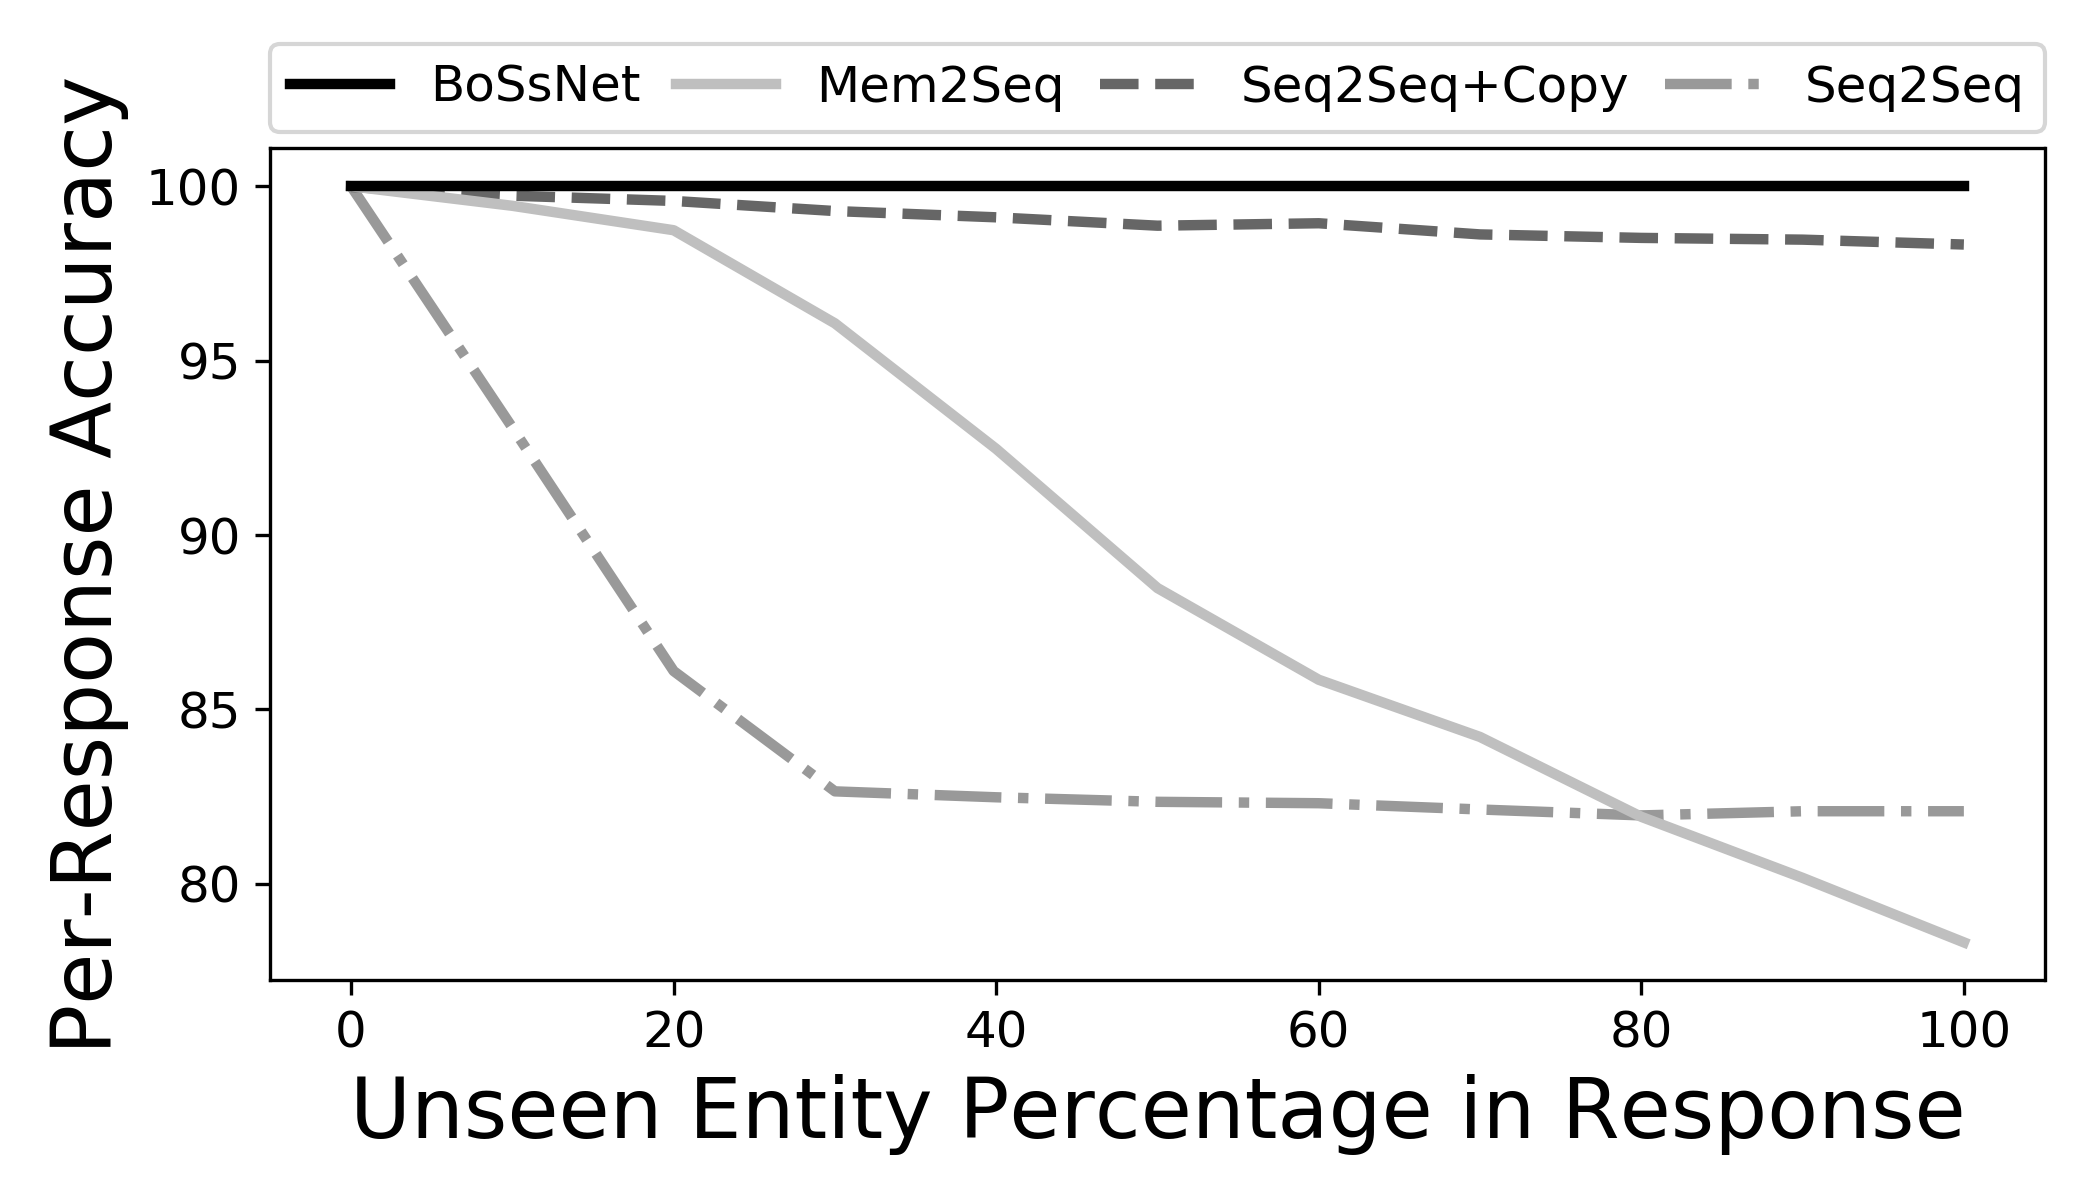
\includegraphics[width=\linewidth]{assets/graphs/task1_Acc.png}
 \caption{}\label{fig:t1Acc}
\end{subfigure}

\vspace*{0.5in}

\begin{subfigure}{0.8\textwidth}
 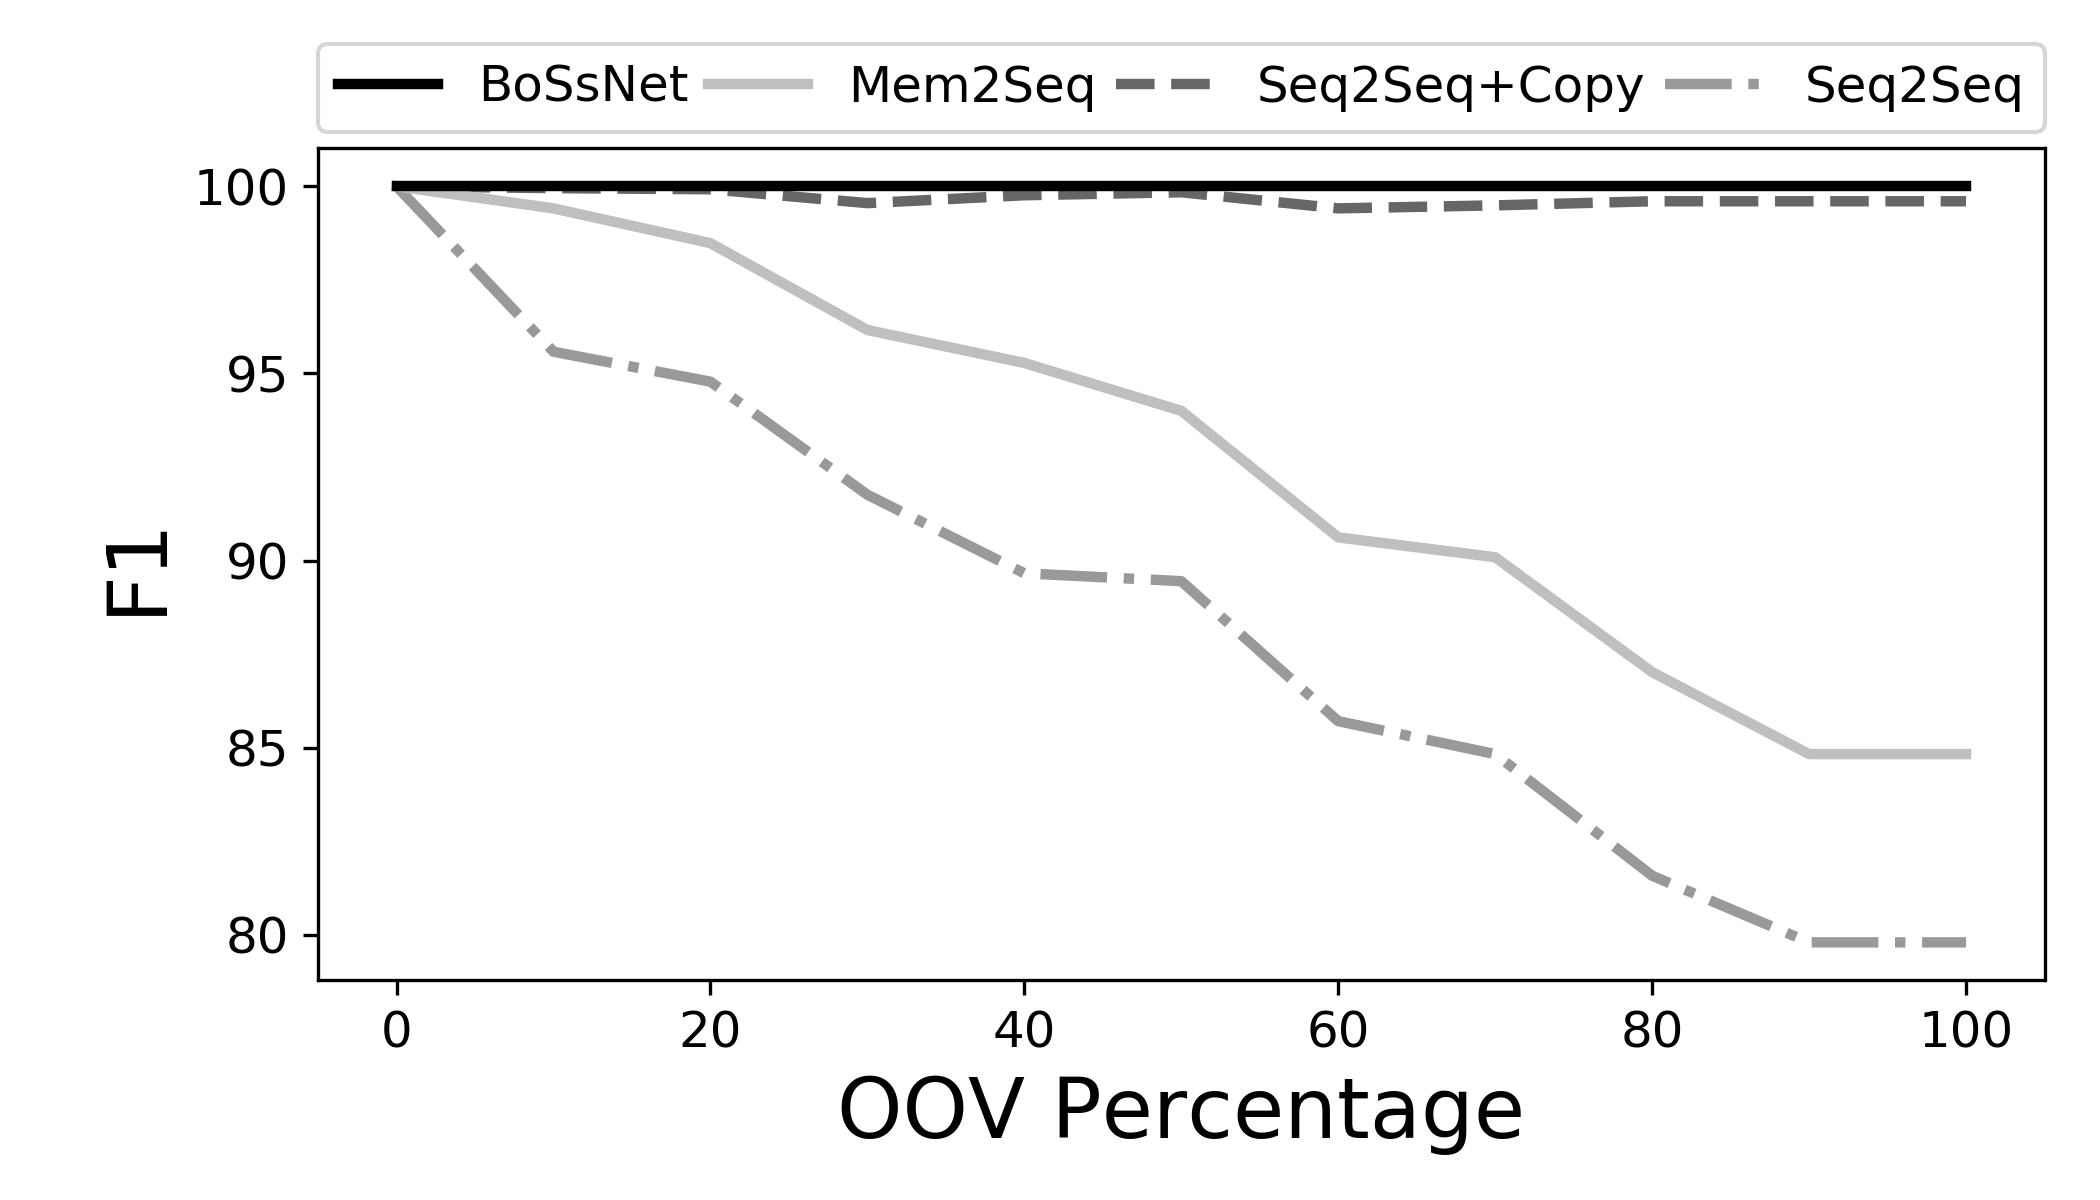
\includegraphics[width=\linewidth]{assets/graphs/task1_F1.png}
 \caption{}\label{fig:t1F1}
\end{subfigure}

\caption{Task 1 Disentanglement Evaluation Plots}
\vspace*{0.5in}

\end{figure}

\clearpage


\begin{figure}[!t]
\centering
\begin{subfigure}{0.8\textwidth}
 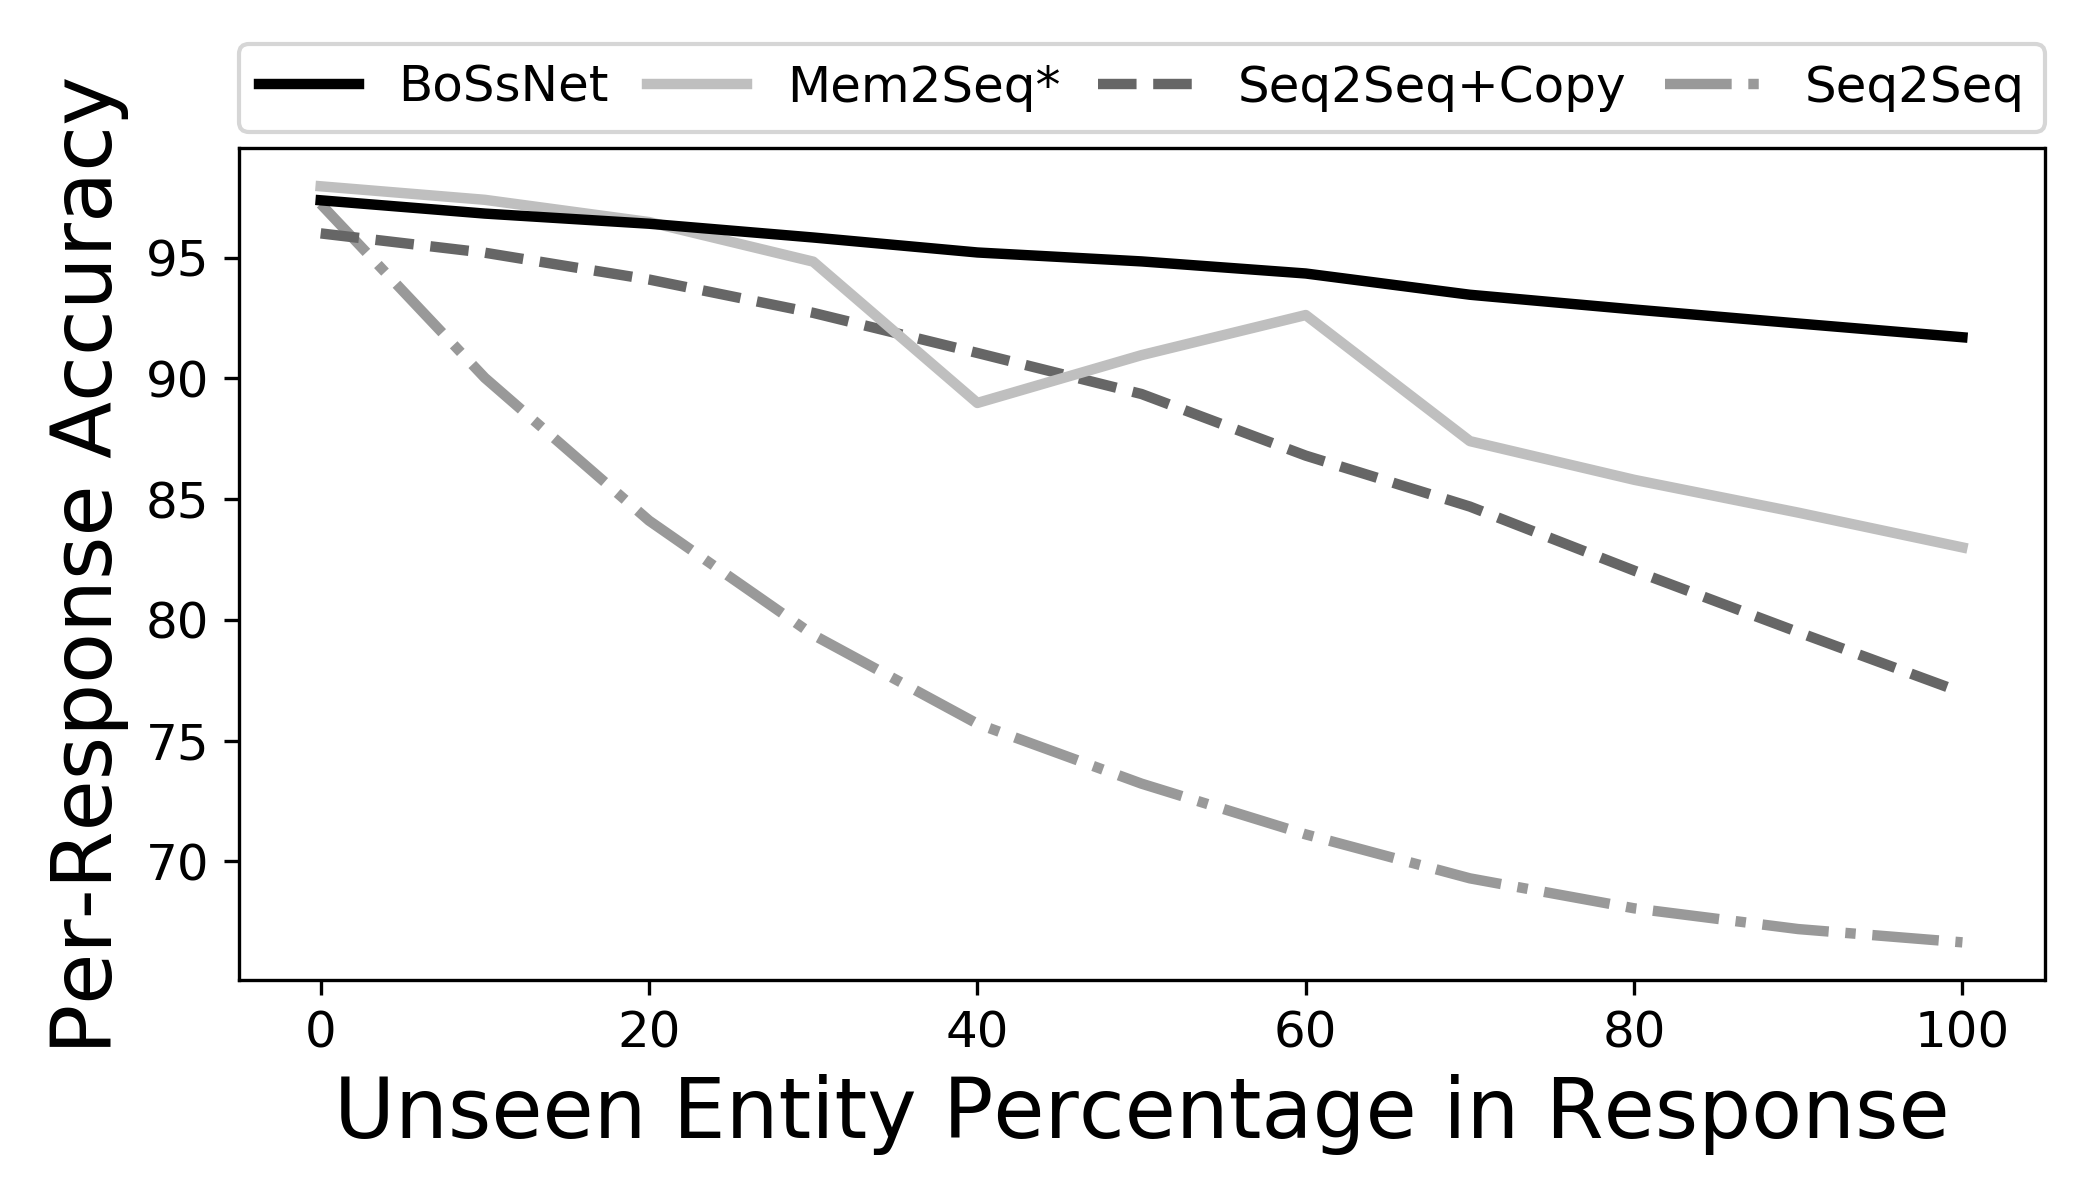
\includegraphics[width=\linewidth]{assets/graphs/task5_Acc.png}
 \caption{}\label{fig:t5Acc}
\end{subfigure}

\vspace*{0.5in}

\begin{subfigure}{0.8\textwidth}
 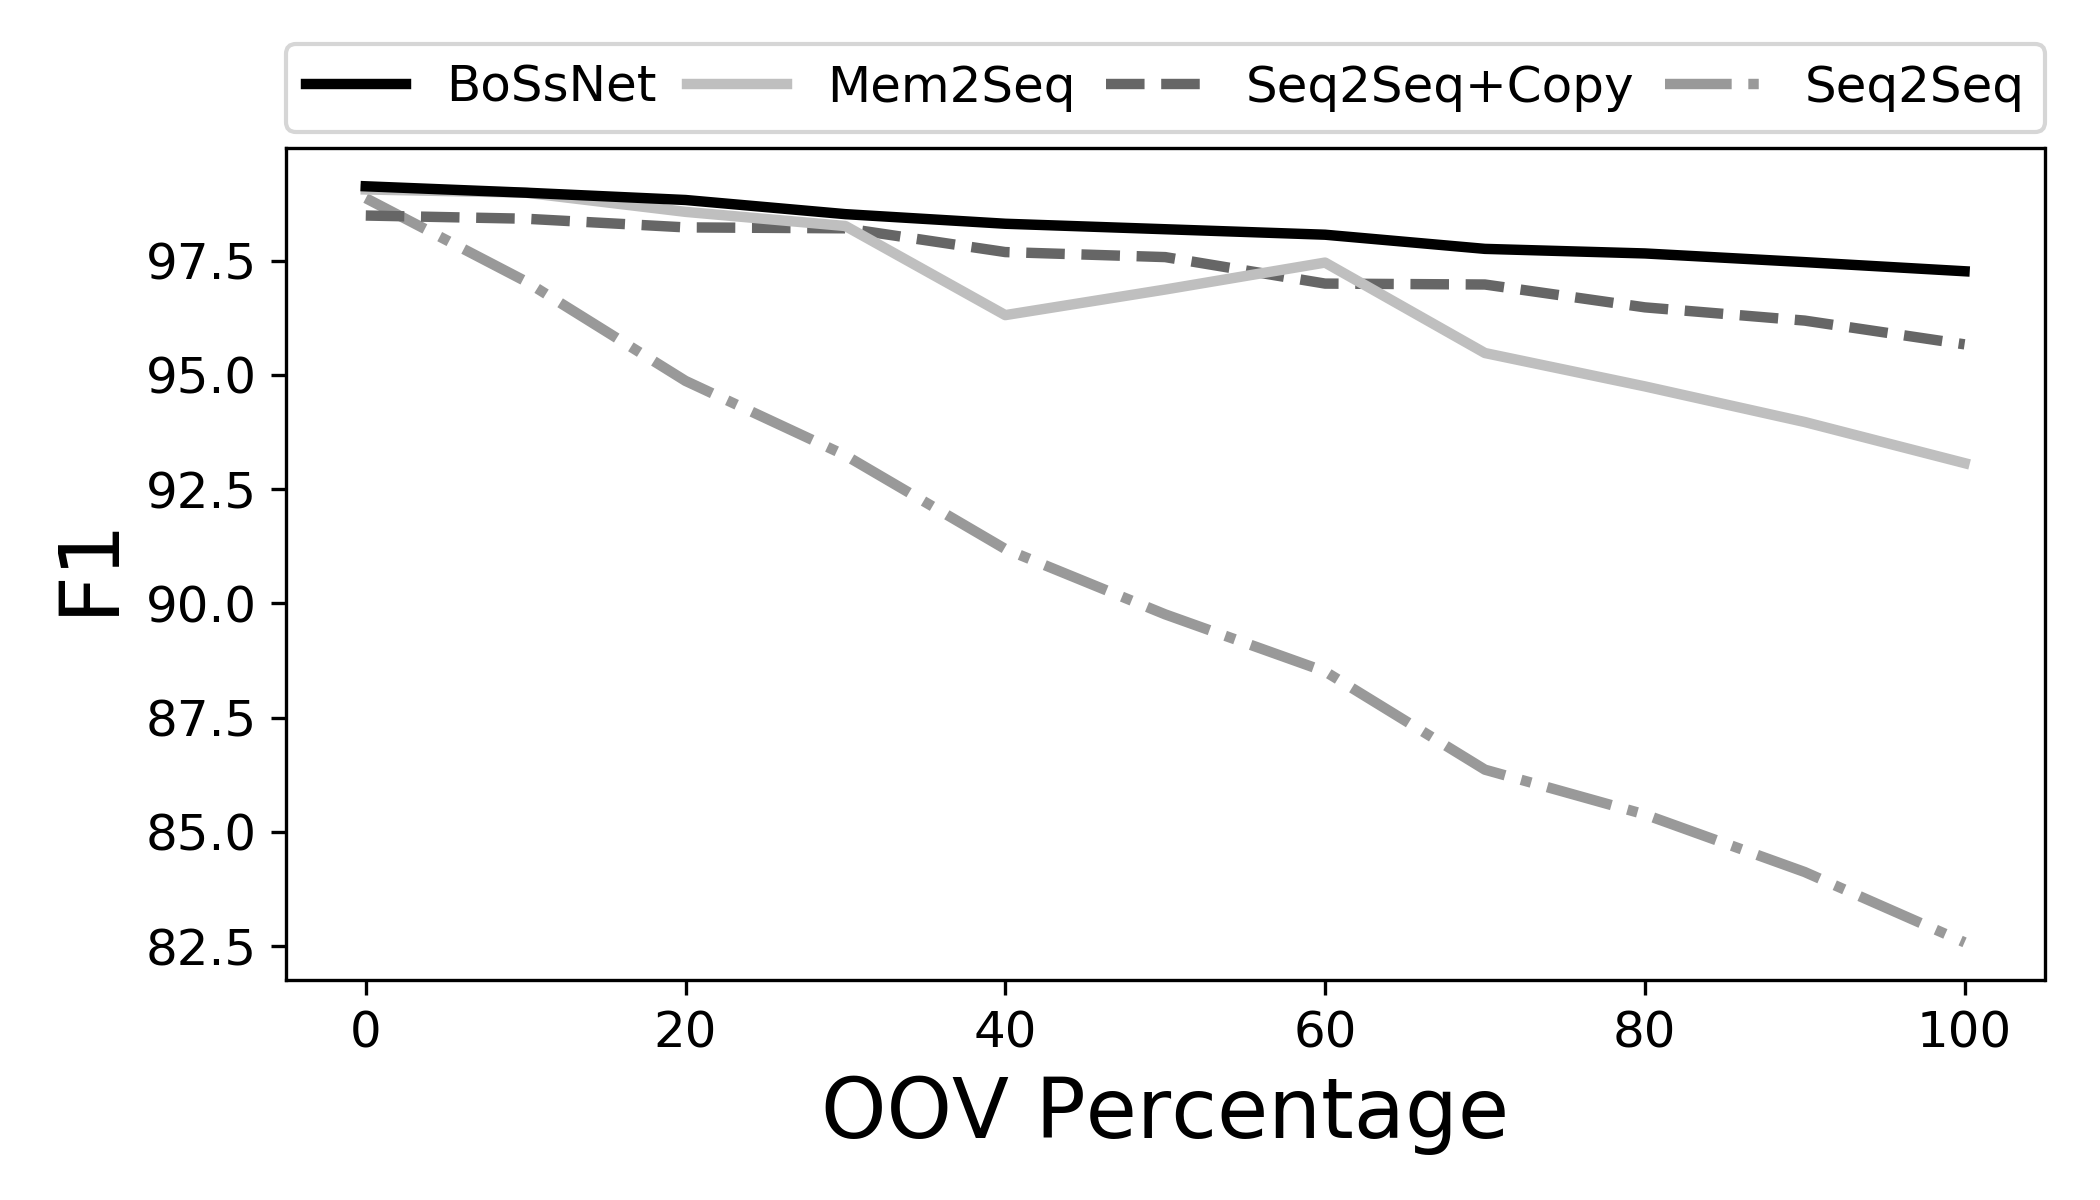
\includegraphics[width=\linewidth]{assets/graphs/task5_F1.png}
 \caption{}\label{fig:t5F1}
\end{subfigure}

\caption{Task 5 Disentanglement Evaluation Plots}
\end{figure}

\clearpage


\begin{figure}[!t]
\centering
\begin{subfigure}{0.8\textwidth}
 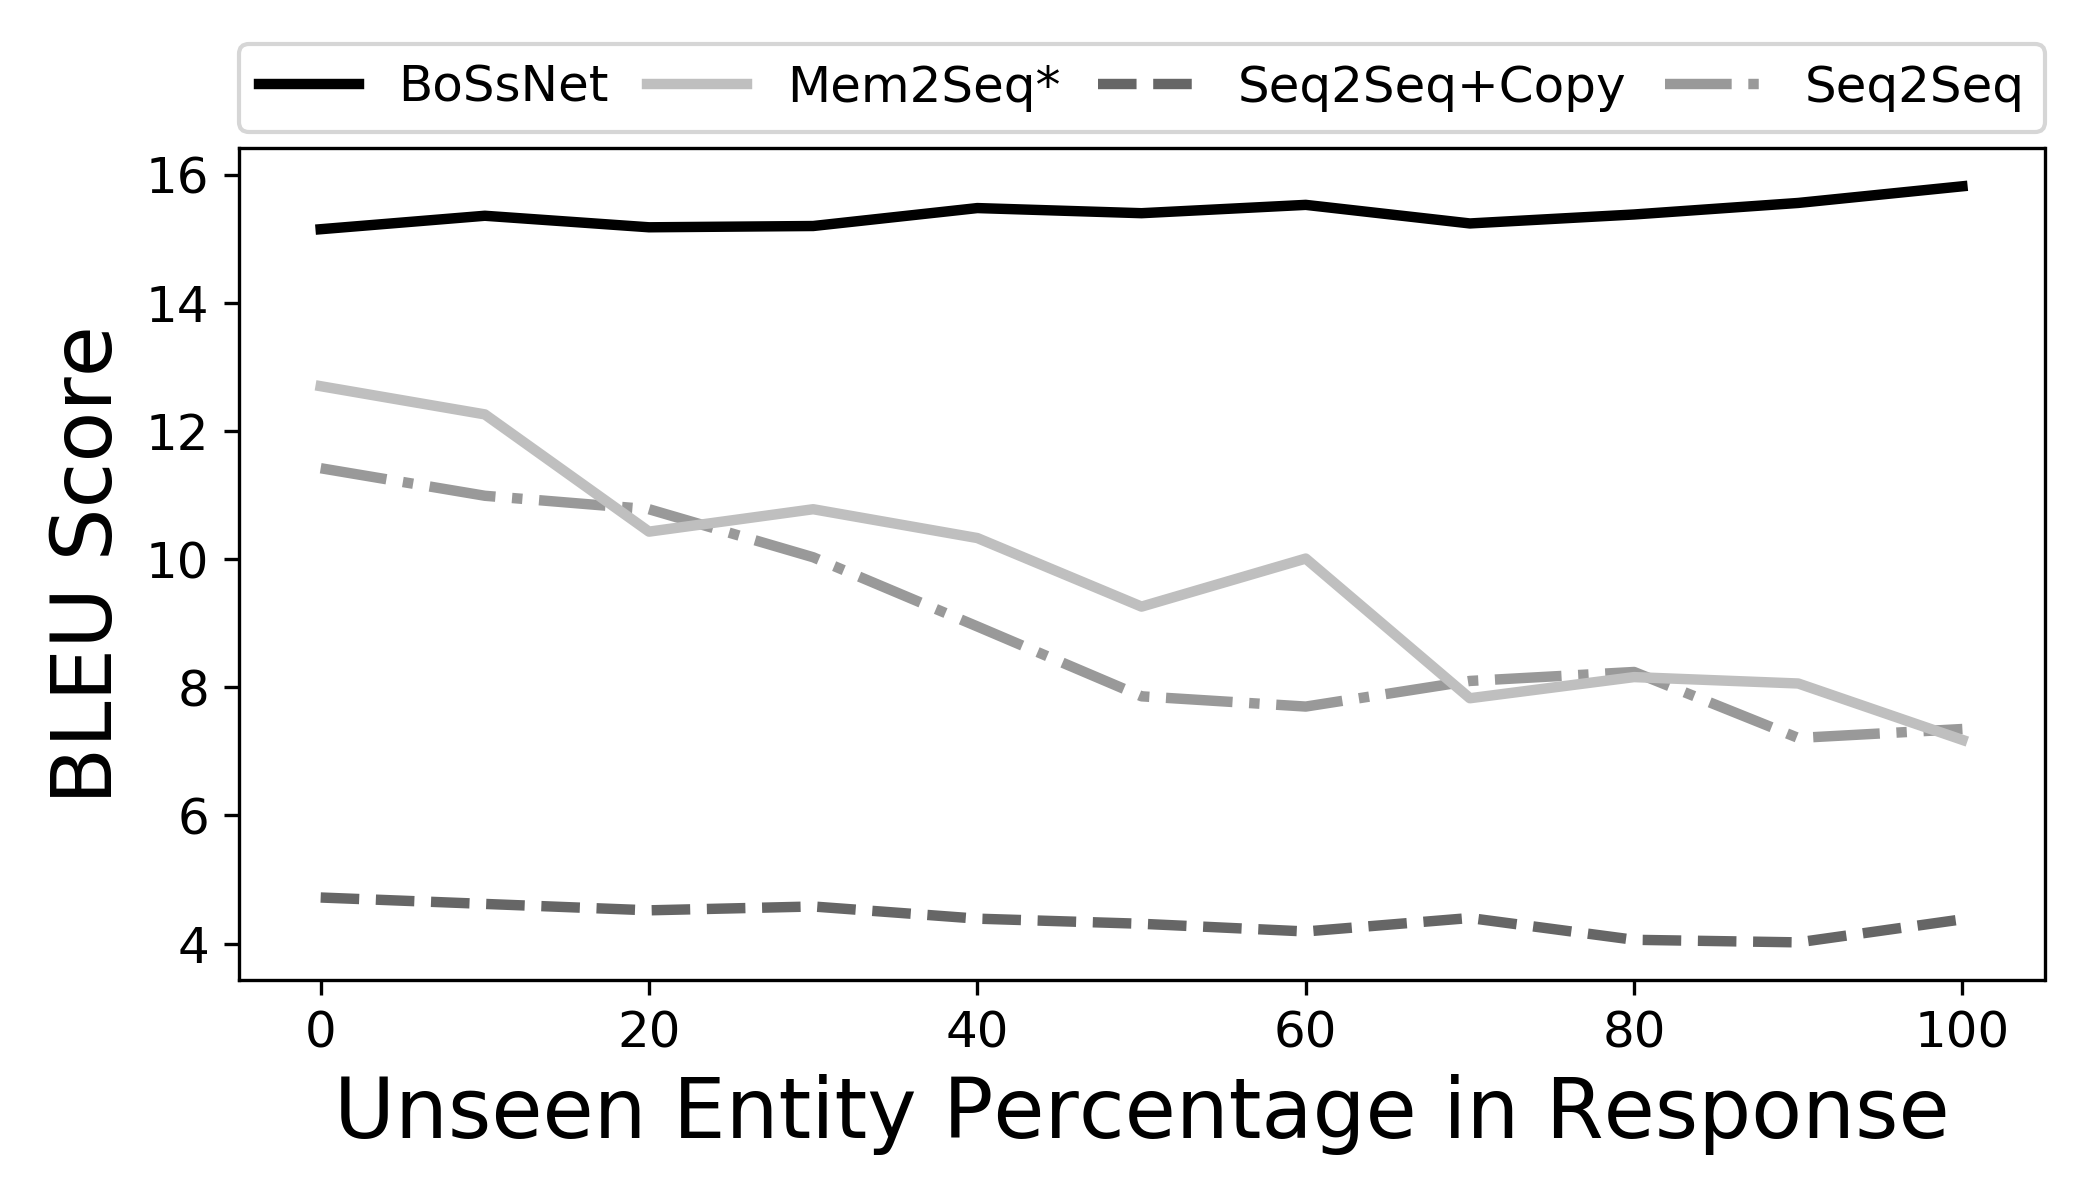
\includegraphics[width=\linewidth]{assets/graphs/camrest_BLEU.png}
 \caption{}\label{fig:camBleu}
\end{subfigure}

\vspace*{0.5in}

\begin{subfigure}{0.8\textwidth}
 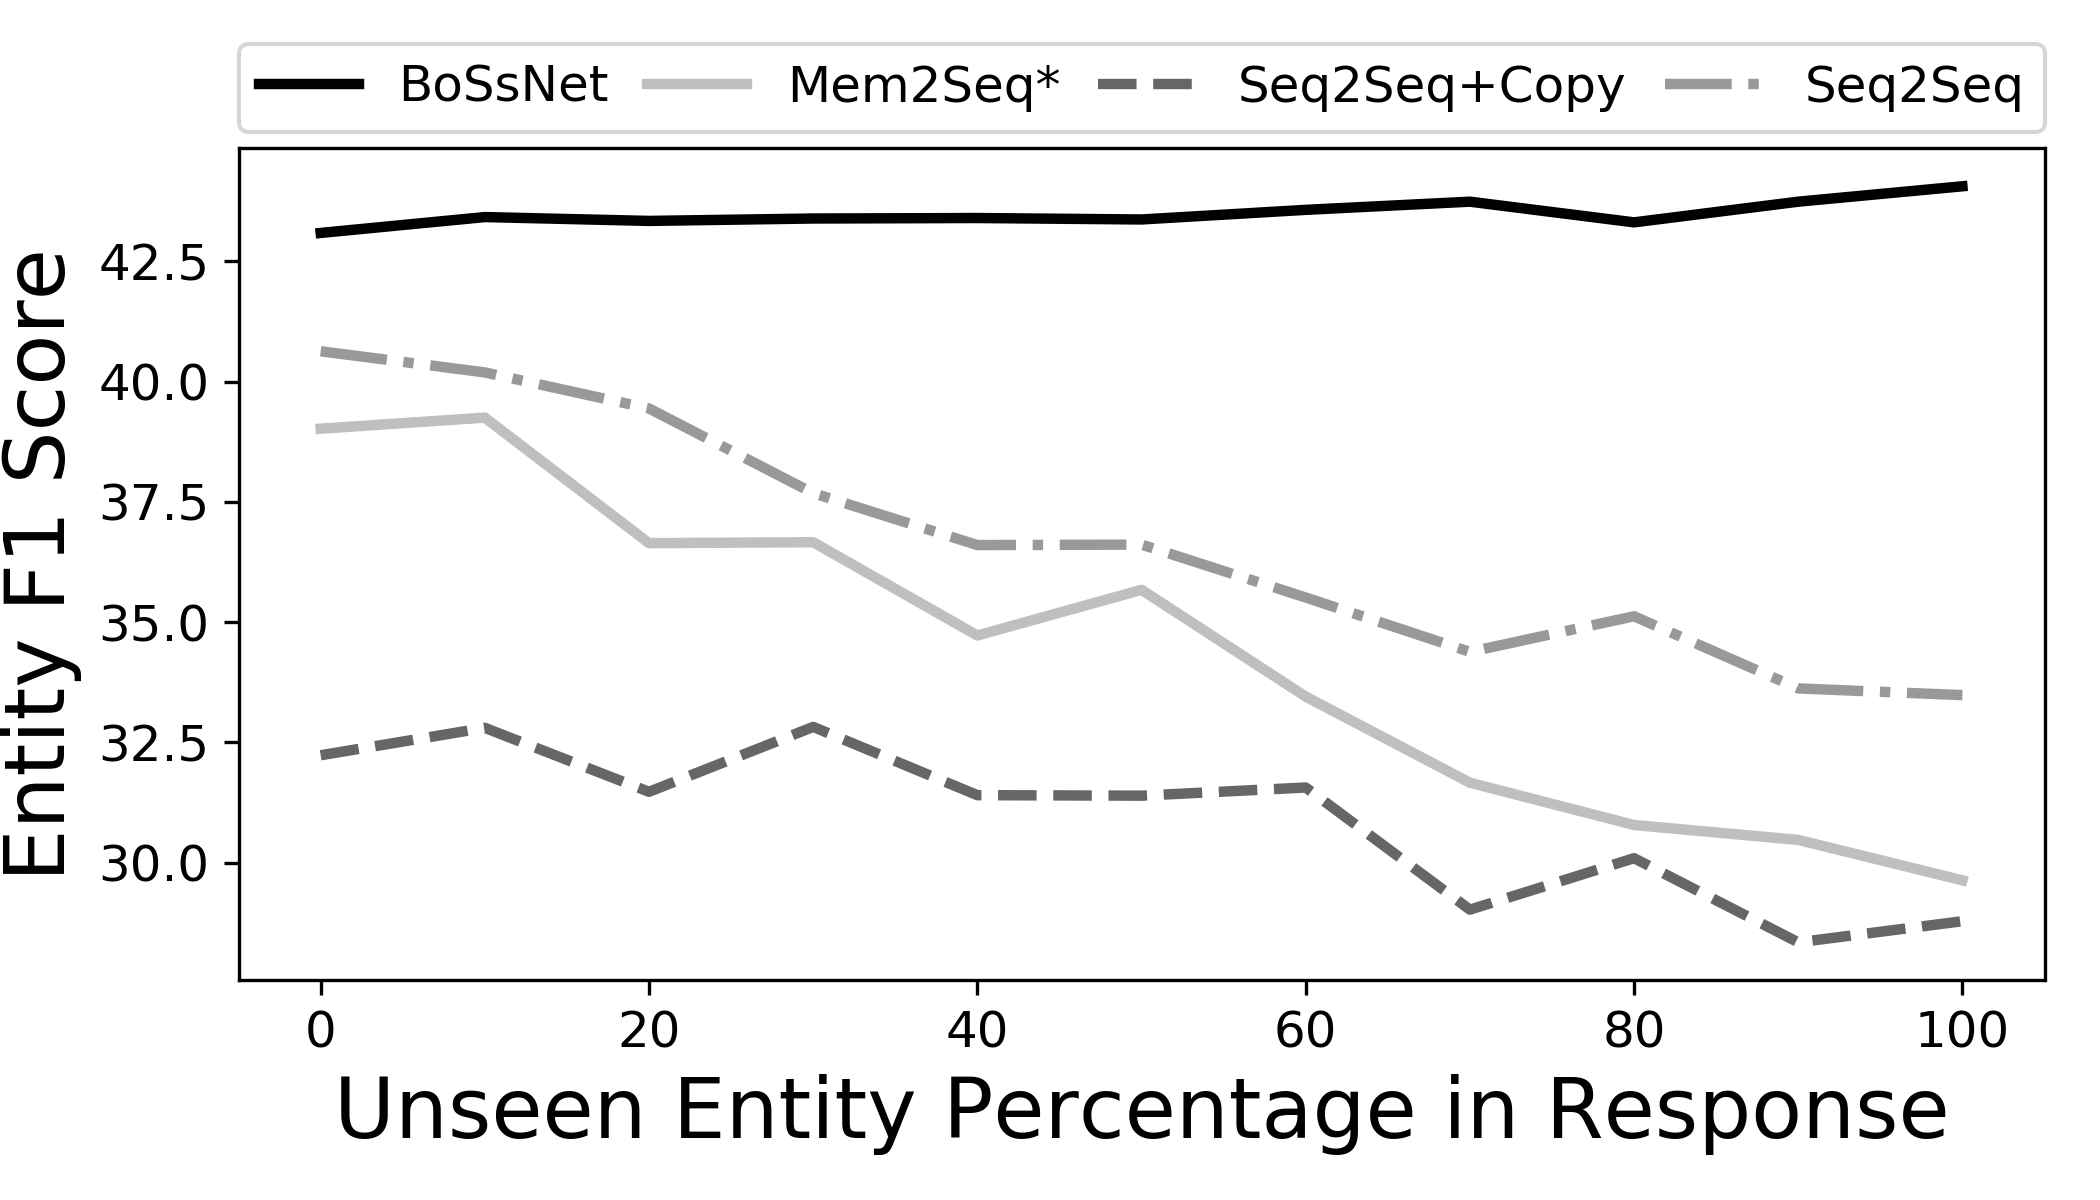
\includegraphics[width=\linewidth]{assets/graphs/camrest_F1.png}
 \caption{}\label{fig:camF1}
\end{subfigure}

\caption{CamRest Disentanglement Evaluation Plots}
\end{figure}

\clearpage


\begin{figure}[!t]
\centering
\begin{subfigure}{0.8\textwidth}
 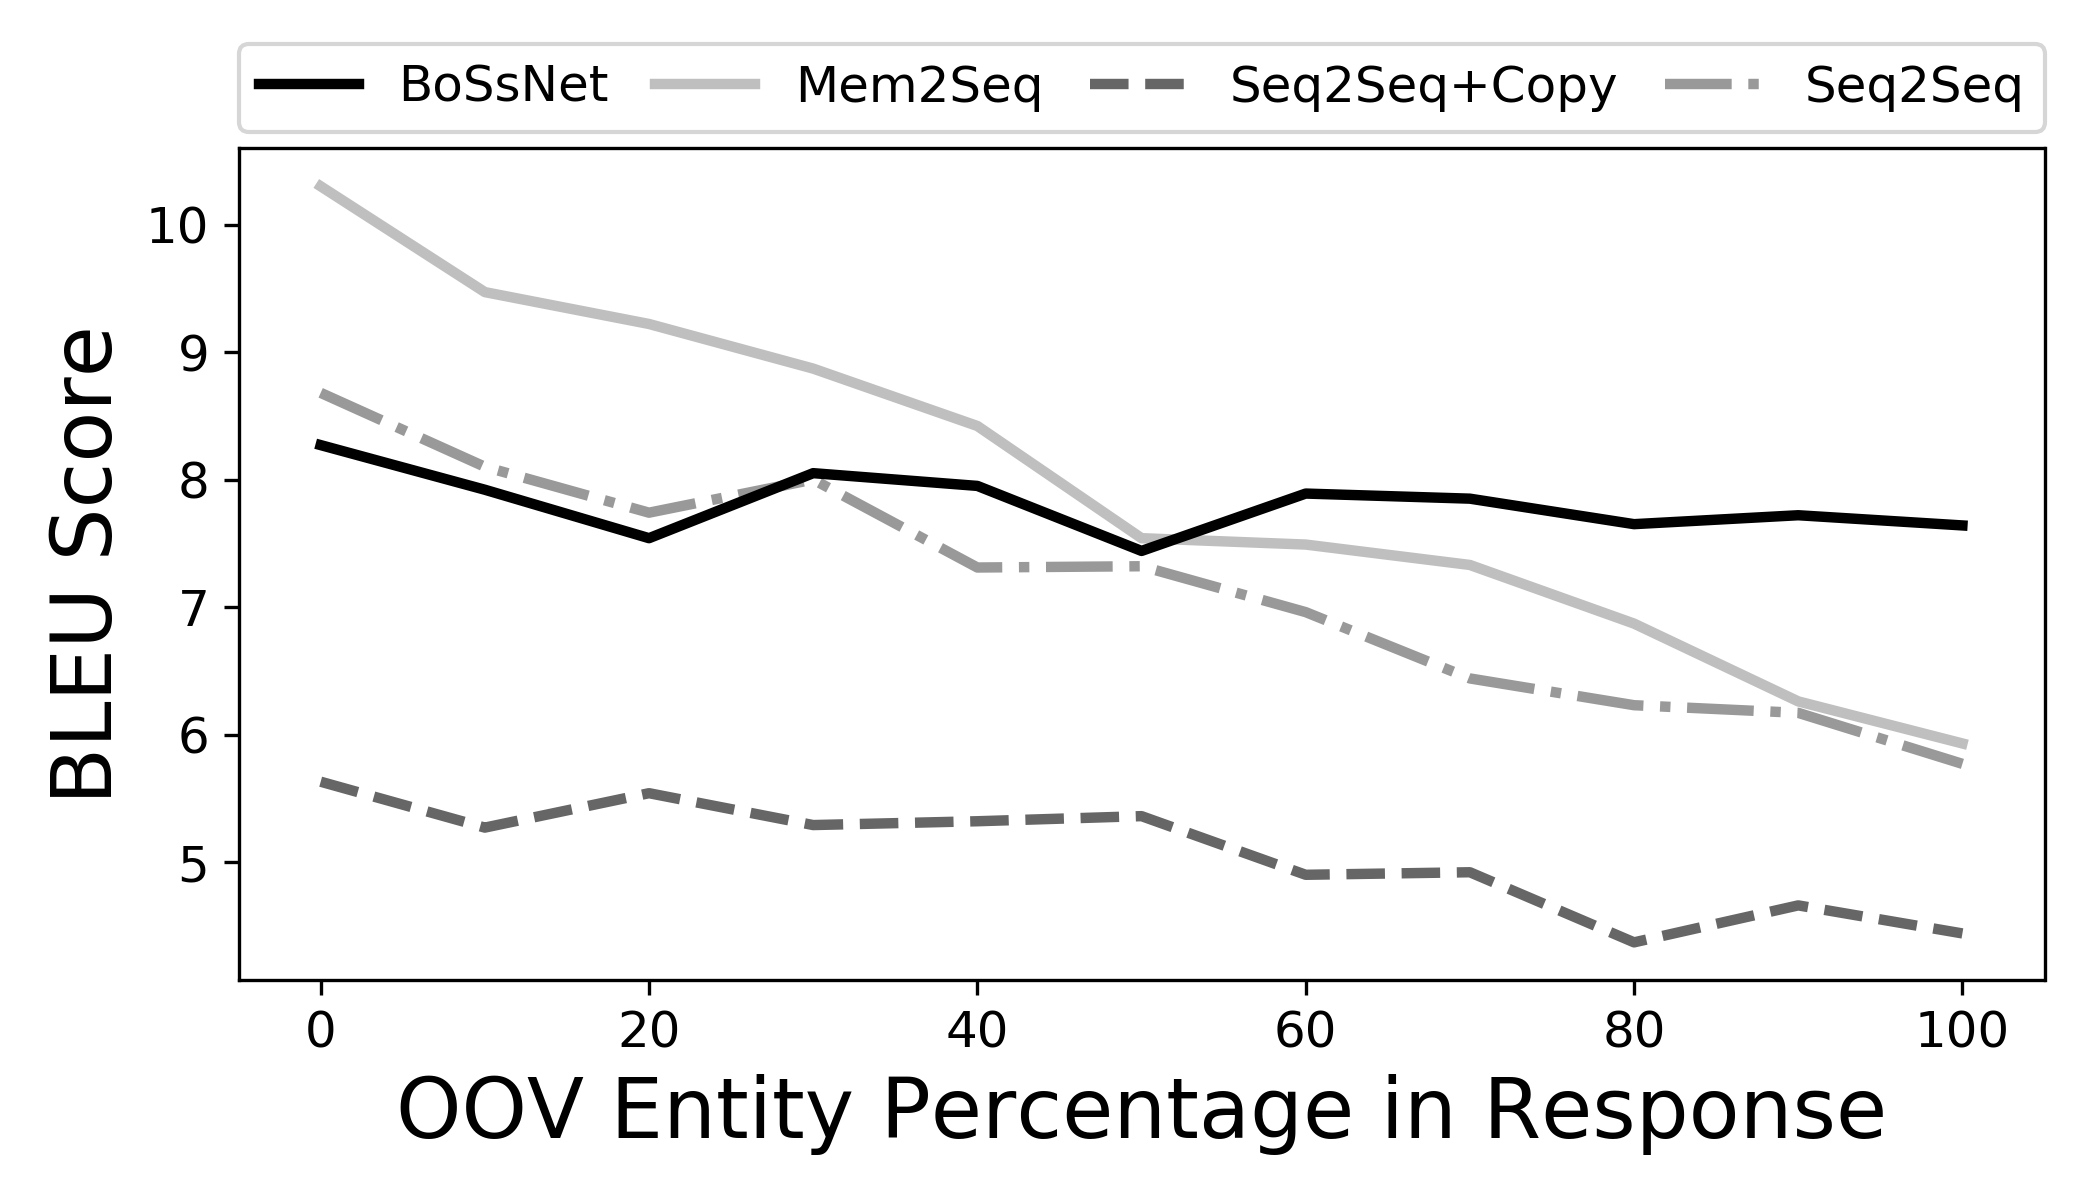
\includegraphics[width=\linewidth]{assets/graphs/smd_BLEU.png}
 \caption{}\label{fig:smdBleu}
\end{subfigure}

\vspace*{0.5in}

\begin{subfigure}{0.8\textwidth}
 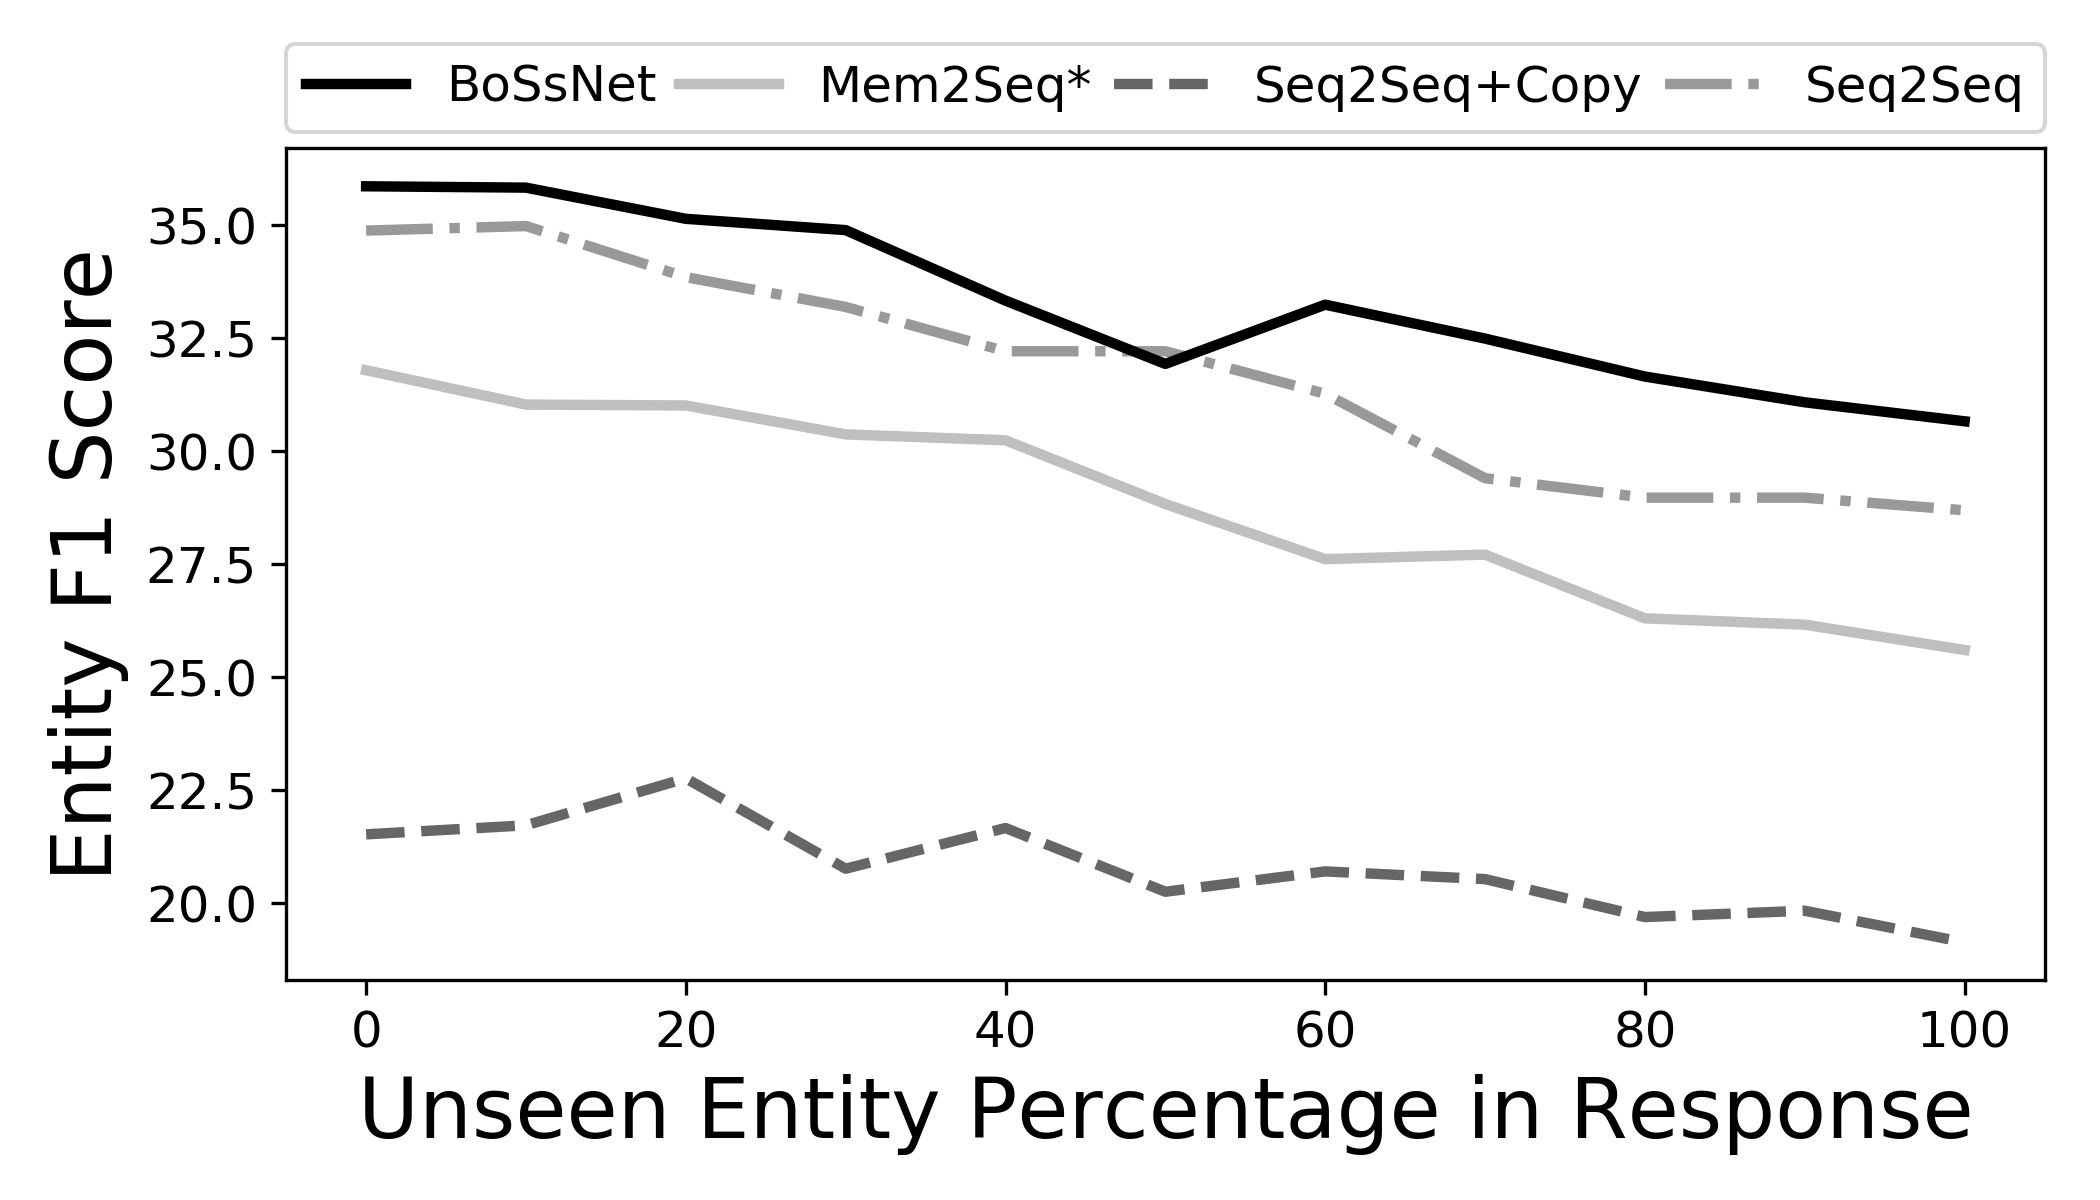
\includegraphics[width=\linewidth]{assets/graphs/smd_F1.png}
 \caption{}\label{fig:smdF1}
\end{subfigure}

\caption{SMD Disentanglement Evaluation Plots}
\end{figure}

\clearpage

% \begin{table}[t]
% \centering
% \footnotesize
%  \begin{tabular}{l|cc|c|cc|c}
% \toprule
% & \multicolumn{3}{c|}{\textbf{CamRest676}} & \multicolumn{3}{c}{\textbf{SMD}}  \\ \cmidrule{2-7}
% & \textbf{0\%} & \textbf{50\%} & \textbf{Total} & \textbf{0\%} & \textbf{50\%} & \textbf{Total} \\
% \midrule
% Seq2Seq & 46 & 26 & 72 & 35 & 22 & 57 \\
% Seq2Seq+Copy & 27 & 22 & 49 & 21 & 16 & 37 \\
% Mem2Seq & 51 & 35 & 86 & \textbf{38} & 26 & 64 \\
% \midrule
% \sys\ & \textbf{77} & \textbf{80} & \textbf{157} & 36 & \textbf{51} & \textbf{87} \\

% \bottomrule
% \end{tabular}
% \caption{AMT Evaluations on CamRest676 and In-car Assistant datasets} 
% \label{tab:amt}
% \end{table}

% \begin{table}[t]
% \centering
% \footnotesize
%  \begin{tabular}{l|cc|cc}
% \toprule
% & \multicolumn{2}{c|}{\textbf{CamRest676}} & \multicolumn{2}{c}{\textbf{SMD}}  \\ \cmidrule{2-5}
% & \textbf{0\%} & \textbf{50\%} &  \textbf{0\%} & \textbf{50\%}\\
% \midrule
% Seq2Seq & 2.24 & 2.28 & 2.38 & \textbf{2.44} \\
% Seq2Seq+Copy & 1.1 & 1.04 & 2.0 & 1.04 \\
% Mem2Seq & 2.2 & 2.06 & 2.0 & 1.9  \\
% \midrule
% \sys\ & \textbf{2.28} & \textbf{2.44} & \textbf{2.5} & 2.28 \\


% \bottomrule
% \end{tabular}
% \caption{AMT Grammar Evaluations on CamRest676 and In-car Assistant datasets} 
% \label{tab:amtg}
% \end{table}

% \begin{figure*}
% \centering
% \begin{minipage}[b]{.475\textwidth}
% 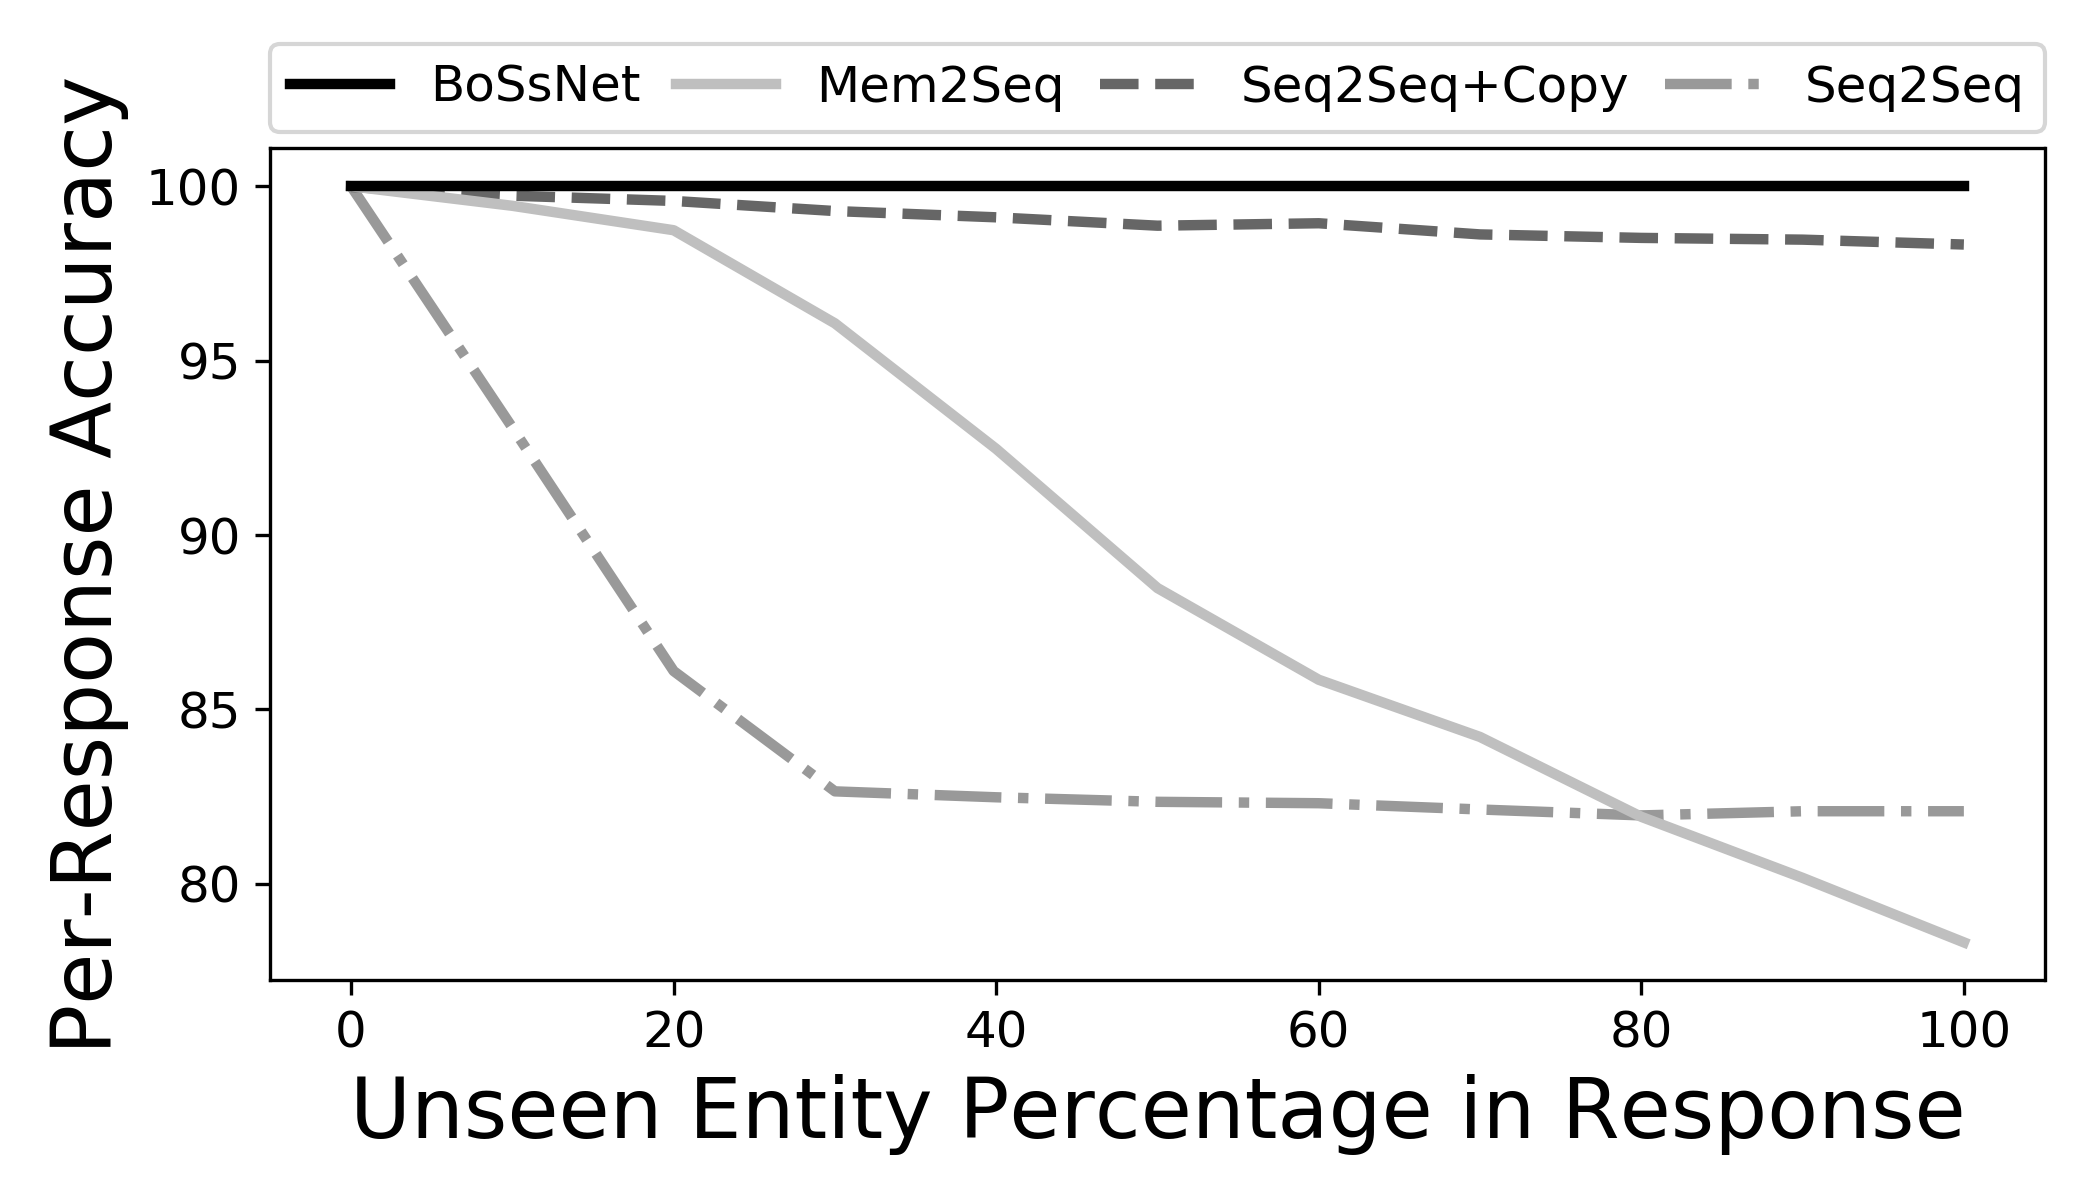
\includegraphics[width=\textwidth, height=4.7cm]{assets/graphs/task1_Acc.png}
% \caption{bAbI Task 1: Per-response accuracy comparison on KA sets}\label{label-a}
% \end{minipage}\qquad
% \begin{minipage}[b]{.475\textwidth}
%  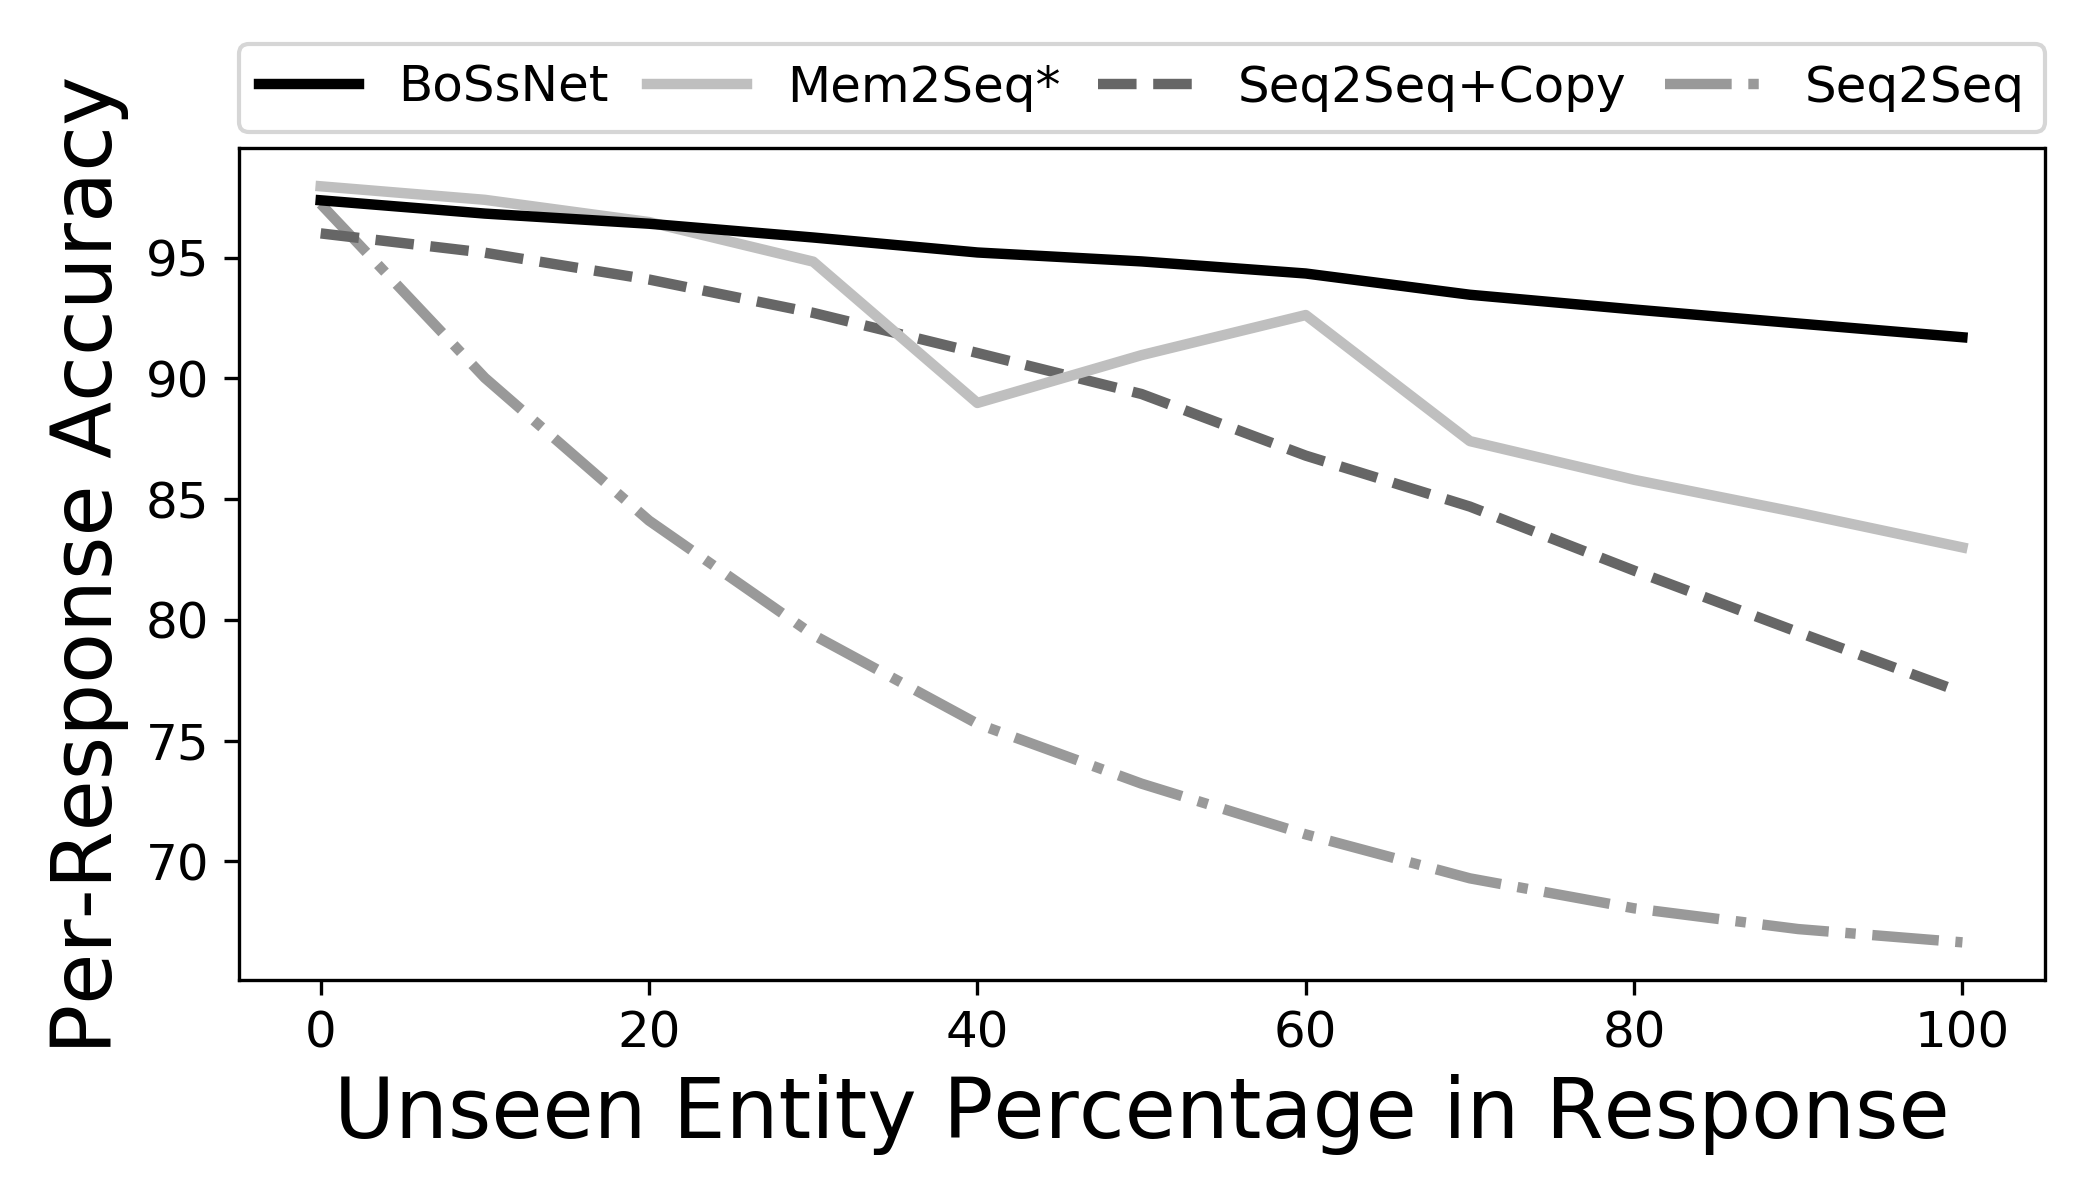
\includegraphics[width=\textwidth, height=4.7cm]{assets/graphs/task5_Acc.png}
%         \caption{bAbI Task 5: Per-response accuracy comparison on KA sets}\label{label-b}
% \end{minipage}
% \end{figure*}

% \begin{figure*}
% \centering
% \begin{minipage}[b]{.475\textwidth}
% 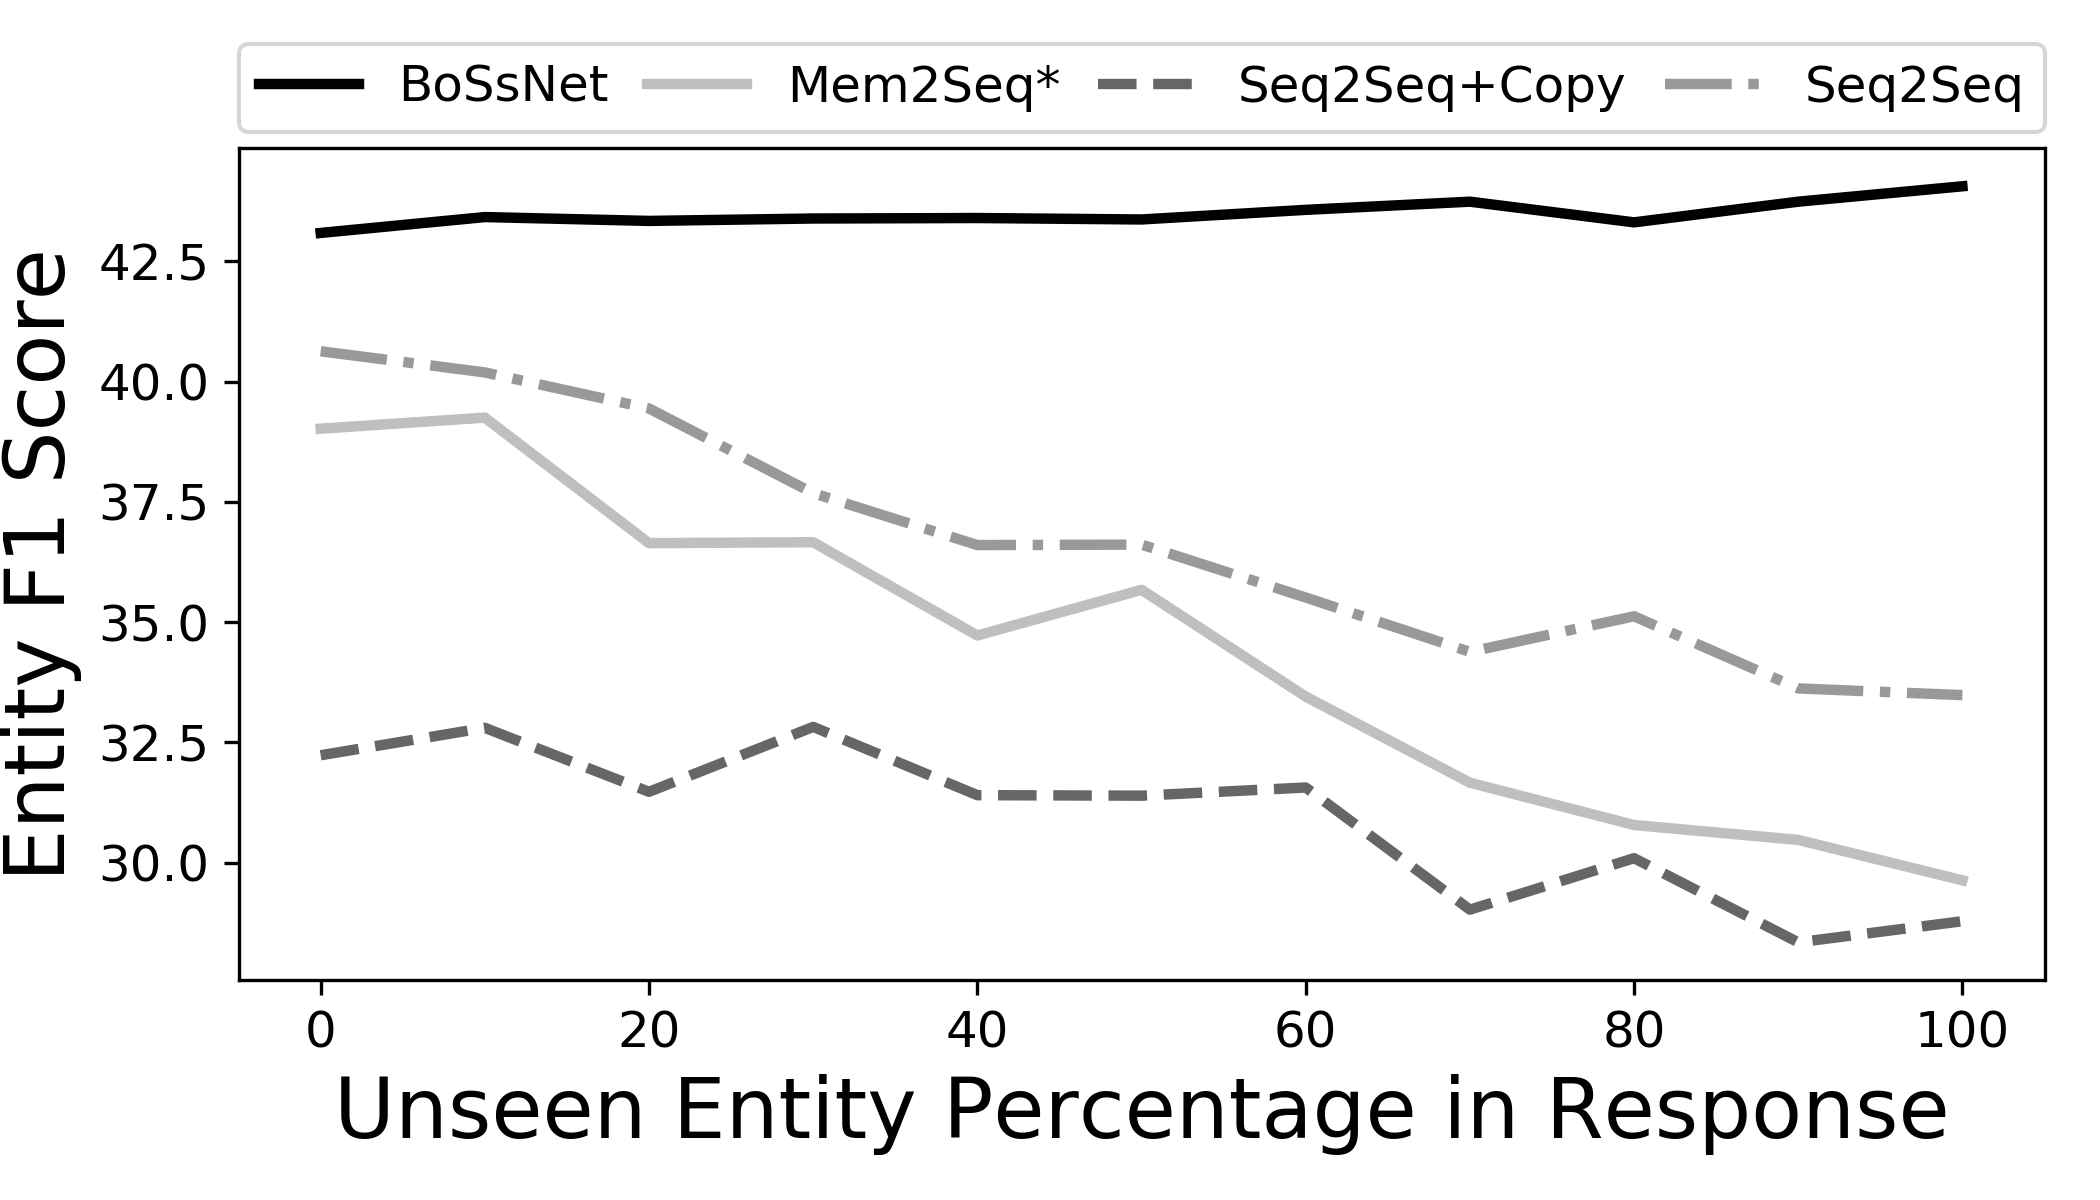
\includegraphics[width=\textwidth, height=4.7cm]{assets/graphs/camrest_F1.png}
% \caption{CamRest: Entity F1 comparison on KA sets}\label{label-c}
% \end{minipage}\qquad
% \begin{minipage}[b]{.475\textwidth}
%  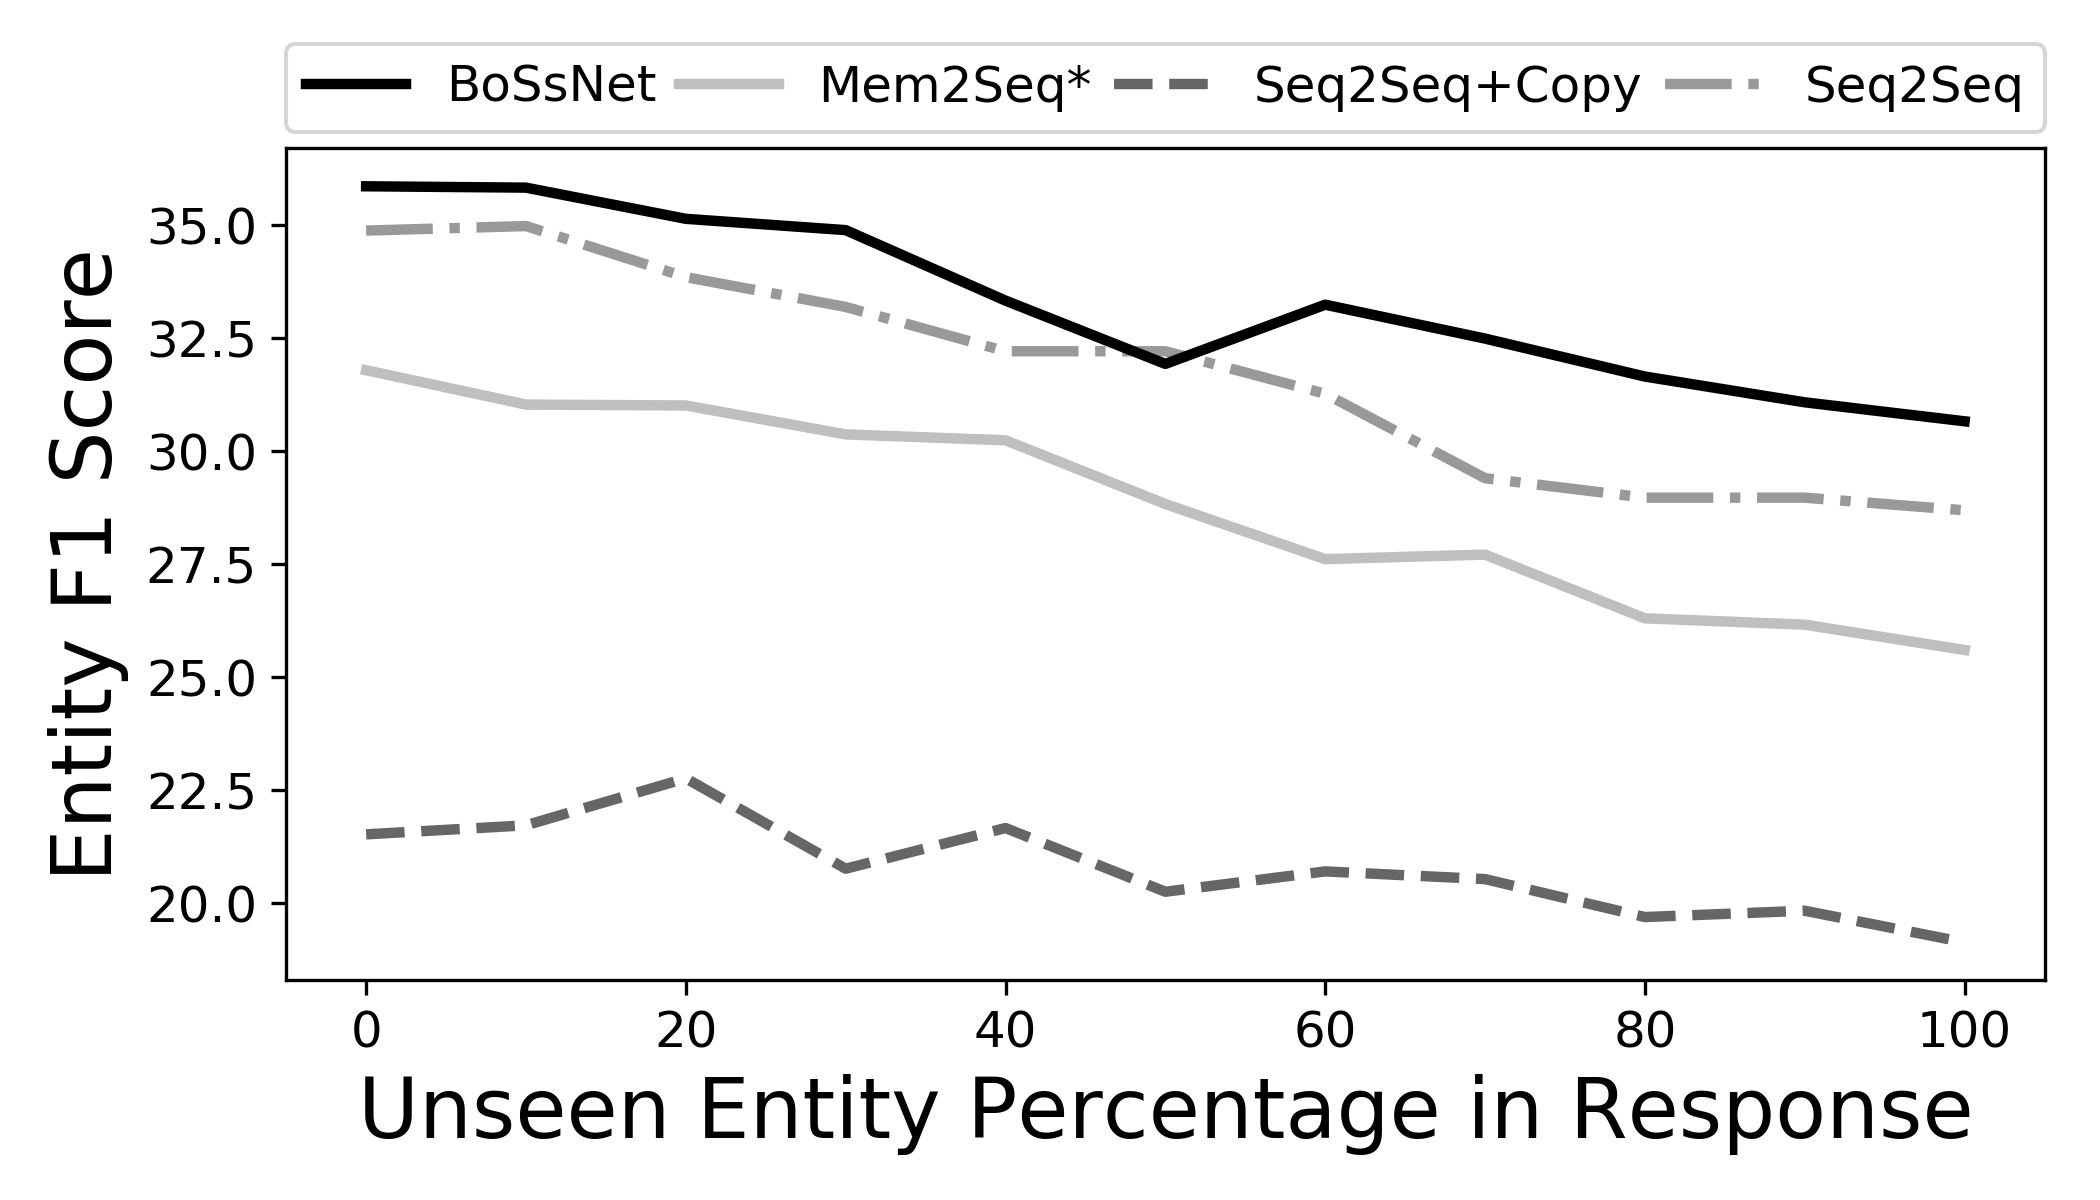
\includegraphics[width=\textwidth, height=4.7cm]{assets/graphs/smd_F1.png}
% \caption{SMD: Entity F1 comparison on KA sets}\label{label-d}
% \end{minipage}
% \end{figure*}

\subsection{Ablation Study}
\label{sec:expt3}

% \begin{table*}[!ht]
% \centering
% \footnotesize
% % \vspace{2mm}
% \begin{tabular}{l|ccccc|ccccc|cc}
% \toprule
%    & \multicolumn{5}{c|}{\textbf{bAbI Dialog Tasks}} & \multicolumn{5}{c|}{\textbf{bAbI Dialog Tasks (OOV)}}  & \multicolumn{2}{c}{\textbf{CamRest}} \\ \cmidrule{2-6} \cmidrule{7-11} \cmidrule{12-13}
%     & T1  & T2  & T3   & T4   & T5   & T1 & T2 & T3 & T4 & T5 & BLEU        & Ent. F1       \\ \midrule
% \sys\ w/o {\sc BoSs} Memory & 100 & 100 & 74.9 & 57.2 & 95.6 & 93.5   & 78.9   & 74.9   & 57     & 81.4   & 10.13        & 29          \\
% \sys\ w/o $\mathcal{L}_{d}$          & 100 & 100 & 91.7 & 100  & 94.3 & 83.2   & 78.9   & 92.7   & 100    & 66.7   & 15.5        & 40.1          \\
% \sys\  w/o DLD     & 100 & 100 & 93.4 & 100  & 95.3 & 79.2   & 84.6   & 90.7   & 100    & 78.1   & 12.4        & 40.45         \\ \midrule
% \sys\                 & 100 & 100 & 95.2 & 100  & 97.3 & 100    & 100    & 95.7   & 100    & 91.7   & 15.2        & 43.1    
% \\ \bottomrule
% \end{tabular}
% \caption{Ablation study: impact of each model element on \sys\ }
% \label{tab:ablation}
% \end{table*}
We assess the value of each model element, by removing it from \sys. Table \ref{tab:ablation} reports the per-response accuracy scores for various configurations of \sys\ on bAbI dialog tasks. It also reports the BLEU and entity F1 metric of various configurations on CamRest.

\noindent \textbf{Without BoSs Memory:} 
This configuration uses the Bag-of-Bags (BoB) Memory rather than {\sc BoSs} memory. The BoB memory is a simplified representation, similar to the one in the original Memory Networks. Here the token representation is the vector embedding of the token with no influence from the surrounding words and the memory cell representation is the sum of all its token embeddings. As a result, each word $w$ representation is influenced equally by all words in a memory cell, irrespective of its distance from $w$. This makes capturing context in the immediate neighbourhood harder. Inability to capture the correct context prevents the configuartion from generalizing to OOV test sets.

\noindent \textbf{Without Disentangled Loss:} Disentangled Loss ($\mathcal{L}_{d}$) plays an important role in enforcing that KB words be copied and other language be generated. By removing this loss component, 
%the system will not enforce copying only KB words in the response. When compared with \sys, 
it achieves better BLEU score in CamRest, but with a drop in Entity F1. Without the disentangled loss, the model sometimes learns to generate KB words. This severely affects OOV performance. As described earlier, an error in bAbI dataset construction tasks 3 and 4 effectively injects the validation set with a lot of OOVs. This anomaly in conjunction with the dropout (DLD), helps the configuration in achieving an acceptable performance for those tasks.

\noindent \textbf{Without Disentangled Label Dropout:} 
\sys\ learns to generate language and copy KB words. Without DLD, the model learns to memorize words to be copied rather than learning the context under which a word should be copied. Hence, the performance on OOV test sets is much inferior compared to the non-OOV setting.

Overall, we notice that combining all three model elements is necessary in obtaining the best performance across all tasks.

\vspace{1cm}

\noindent \textbf{Multi-Hop vs 1-Hop Encoders:}
Table \ref{tab:ablationhop} shows the performance of bAbI tasks and CamRest on two \sys\ encoder settings. Multi-hops in encoder helps in bAbI task 3 and 5, as they require inferencing over the KB tuples (sorting restaurants by rating) to recommend a restaurant. We also see substantial improvements on CamRest in both BLEU and entity F1 metric.

\begin{table}
\centering
\footnotesize
% \vspace{2mm}
\begin{tabular}{l|c|c|c}
\toprule
   & \textbf{bAbI Dialog} & \textbf{bAbI Dialog (OOV)}  & \textbf{CamRest} \\ \cmidrule{2-4}
    & Avg. Response Acc.  & Avg. Response Acc. & Ent. F1       \\ \midrule
\sys\ w/o {\sc BoSs} Memory & 85.54 & 77.14 & 29          \\
\sys\ w/o $\mathcal{L}_{d}$          & 97.2 & 84.3 & 40.1          \\
\sys\  w/o DLD     & 97.74 & 86.52 & 40.45         \\ \midrule
\sys\                 & 98.5    & 97.48 & 43.1    
\\ \bottomrule
\end{tabular}
\caption{Ablation study: impact of each model element on \sys\ }
\label{tab:ablation}
\end{table}

\begin{table}
\centering
\footnotesize
\begin{tabular}{l|ccccc|ccccc|cc}
\toprule
   & \multicolumn{5}{c|}{\textbf{bAbI Dialog Tasks}} & \multicolumn{5}{c|}{\textbf{bAbI Dialog Tasks (OOV)}}  & \multicolumn{2}{c}{\textbf{CamRest}} \\ \cmidrule{2-6} \cmidrule{7-11} \cmidrule{12-13}
    & T1  & T2  & T3   & T4   & T5   & T1 & T2 & T3 & T4 & T5 & BLEU        & Ent. F1       \\ \midrule
1-Hop  & 100 & 100 & 92.3 & 100 & 90.5 & 100 & 100 & 91.4 & 100 & 89 & 10.5 & 36.9 \\
Multi-Hop  & 100 & 100 & 95.2 & 100  & 97.3 & 100    & 100    & 95.7   & 100    & 91.7   & 15.2        & 43.1    
\\ \bottomrule
\end{tabular}
\caption{Ablation study: impact of hops in \sys\ encoder }
\label{tab:ablationhop}
\end{table}

%We finally see that, the OOV performance is as comparable to the non-OOV performance when all the elements of \sys\ are combined together.

\begin{table}[!h]

\vspace*{0.5in}

\centering
\small
\begin{tabular}{c|p{13cm}}
\toprule
%\textbf{kb} & \textit{da\_vinci\_pizzeria}\\
% & \textit{r_phone|01223\_351707} \\
% & \textit{r_adddress|20\_milton\_road\_chesterton} \\
% & \textit{r_food|italian} \\
\multicolumn{2}{c}{\textbf{KB (restaurant|cuisine|address|phone)}} \\
\multicolumn{2}{c}{\textit{pizza\_hut\_fen\_ditton}|\textit{italian}|\textit{newmarket\_road\_fen\_ditton}|\textit{01223\_323737}}\\
\midrule
\midrule
\textbf{usr-1} & may i have information for an \textit{italian} restaurant in the \textit{east} part of town ? \\
\textbf{sys-1} & yes sure . there is only on \textit{italian} restaurant called \textit{pizza\_hut\_fen\_ditton} in the \textit{east} . what else do you want to know ? \\
\textbf{usr-2} & what is their address please ? \\
\midrule
\textbf{Gold} & the address for \textit{pizza\_hut\_fen\_ditton} is \textit{newmarket\_road\_fen\_ditton} . can i help you with anything else ?
 \\
\midrule
\midrule
\specialcell[t]{\textbf{Seq2Seq+Copy}} & their address is at
 \\
\midrule
\textbf{Seq2Seq} & \textit{curry\_prince} is at \textit{451\_newmarket\_road\_fen\_ditton} \\

\midrule
\textbf{Mem2Seq} & \textit{pizza\_hut\_fen\_ditton} is located at \textit{7\_barnwell\_road\_fen\_ditton} is \textit{7\_barnwell\_road\_fen\_ditton} and the phone number is \textit{01223\_244955}
 \\
\midrule
\textbf{\sys\ } & \textit{pizza\_hut\_fen\_ditton} is located at \textit{newmarket\_road\_fen\_ditton} is there anything else i can help you with \\
\bottomrule
\end{tabular}
\caption{An example of responses generated by \sys\ and baselines on the CamRest test set. This example has no unseen entities.}
\label{tab:camrest-qualeval}
% \end{table}
\vspace*{0.5in}
% \begin{table}
% \centering
% \small
\begin{tabular}{c|l}
\toprule
\multicolumn{2}{c}{\textbf{KB (restaurant|cuisine|price\_range|location|rating)}} \\
\multicolumn{2}{c}{\textit{resto\_tokyo\_affordable\_vietnamese\_8stars}|\textit{vietnamese}|\textit{affordable}|\textit{tokyo}|\textit{8}}\\
\multicolumn{2}{c}{\textit{resto\_tokyo\_affordable\_vietnamese\_7stars}|\textit{vietnamese}|\textit{affordable}|\textit{tokyo}|\textit{7}}\\
\multicolumn{2}{c}{\textit{resto\_tokyo\_affordable\_vietnamese\_6stars}|\textit{vietnamese}|\textit{affordable}|\textit{tokyo}|\textit{6}}\\
\multicolumn{2}{c}{\textit{resto\_tokyo\_affordable\_vietnamese\_5stars}|\textit{vietnamese}|\textit{affordable}|\textit{tokyo}|\textit{5}}\\
\midrule
\midrule
\textbf{usr-1} & can you book a table in \textit{tokyo} with \textit{vietnamese} food in a \textit{affordable} price range ? \\
\textbf{sys-1} & what do you think of this option : \textit{resto\_tokyo\_affordable\_vietnamese\_8stars} ? \\
\textbf{usr-2} & no this does not work for me . \\
\textbf{sys-2} & what do you think of this option : \textit{resto\_tokyo\_affordable\_vietnamese\_7stars} ? \\
\textbf{usr-3} & do you have something else ? \\
\midrule
\textbf{Gold} & what do you think of this option : \textit{resto\_tokyo\_affordable\_vietnamese\_6stars}
 \\
\midrule
\midrule
\specialcell[t]{\textbf{Seq2Seq+Copy}} & what do you think of this option : what ?
 \\
\midrule
\textbf{Seq2Seq} & what do you think of this option : \textit{resto\_london\_moderate\_british\_2stars} ? \\

\midrule
\textbf{Mem2Seq} & what do you think of this option : \textit{resto\_tokyo\_affordable\_vietnamese\_5stars} ?
 \\
\midrule
\textbf{\sys\ } & what do you think of this option : \textit{resto\_tokyo\_affordable\_vietnamese\_6stars} ? \\
\bottomrule
\end{tabular}
\caption{An example of responses generated by \sys\ and baselines on bAbI dialog Task-5. This example is from the KA test set with 100\% unseen entities.}
\label{tab:task5-qualeval}

\vspace*{0.5in}

\end{table}


\subsection{Qualitative Evaluation}
We qualitatively compare the performance of \sys\ with other baselines using examples.

Table \ref{tab:camrest-qualeval}, demonstrates the ability of \sys\ to copy entities (restaurant name and address) in its response. The other baselines either generate unwanted or irrelevant entities in their response, or fail to copy altogether. \sys\ also best captures the language model effectively with a slight paraphrasing of the gold response.

Table \ref{tab:task5-qualeval} contains only unseen entities. This example highlights the shortcomings of the Seq2Seq model as it ends up predicting a restaurant encountered during training. Mem2Seq copies a restaurant name without learning to sort the restaurants based on rating. \sys, with its efficient memory addressing, is seen to be able to solve both issues.

% \clearpage

\subsection{Visual Evaluation}
\label{ssec:hierarattn}

To visualize the benefit of two-level attention used on {\sc BoSs} memory by the decoder, we compare attention weights for two models: our proposed \emph{two-level attention} and a variant with just \emph{one-level attention} (over all the words in the memory). In the example of a sample dialog from bAbI Task 3, shown in Figure \ref{fig:attention}, the decoder is aimed at predicting the second best restaurant \textit{3 stars}, given that the restaurant with rating \textit{8 stars} has already been suggested and rejected. We show attention only on the KB entries for brevity.

The models share some similarities in their distribution of attention. First, the attention weights are localized over the restaurant names, indicating the preference of the system to point to a specific restaurant. This is supported by the $g_s$ values, $3.14$ x $10^{-5}$ and $1.15$ x $10^{-4}$ for two-level attention and one-level attention respectively, i.e., both models prefer to copy rather than generate. Moreover, entries with the same restaurant name have similar attention weights, reflecting the robustness of the distribution.

We also observe that two-level attention is able to perform the difficult task of {\em sorting} the restaurant entries based on decreasing order of rating (number of stars). It gives more weight to entries with a high rating 
(\textit{3 stars} $>$ \textit{2 stars} $>$ \textit{1 star})
and suppresses the weights of any previously suggested restaurant.
%, e.g., \textit{8 stars}. 

The attention over memory cells provides \sys\ with the ability to infer over multiple sets of tuples. The ability to sort the restaurants and reject a previously seen restaurant can be observed by the attention heat map of Memory cells. Attention over tokens on the other hand can push the attention weights towards either the subject or object in the KB tuple, based on the query's request. Thus using both in conjunction helps \sys\ perform significantly better than the baselines and illustrates the importance of the {\sc BoSs} memory in comparison to a flat memory layout.

\begin{figure*}[ht]
\centering
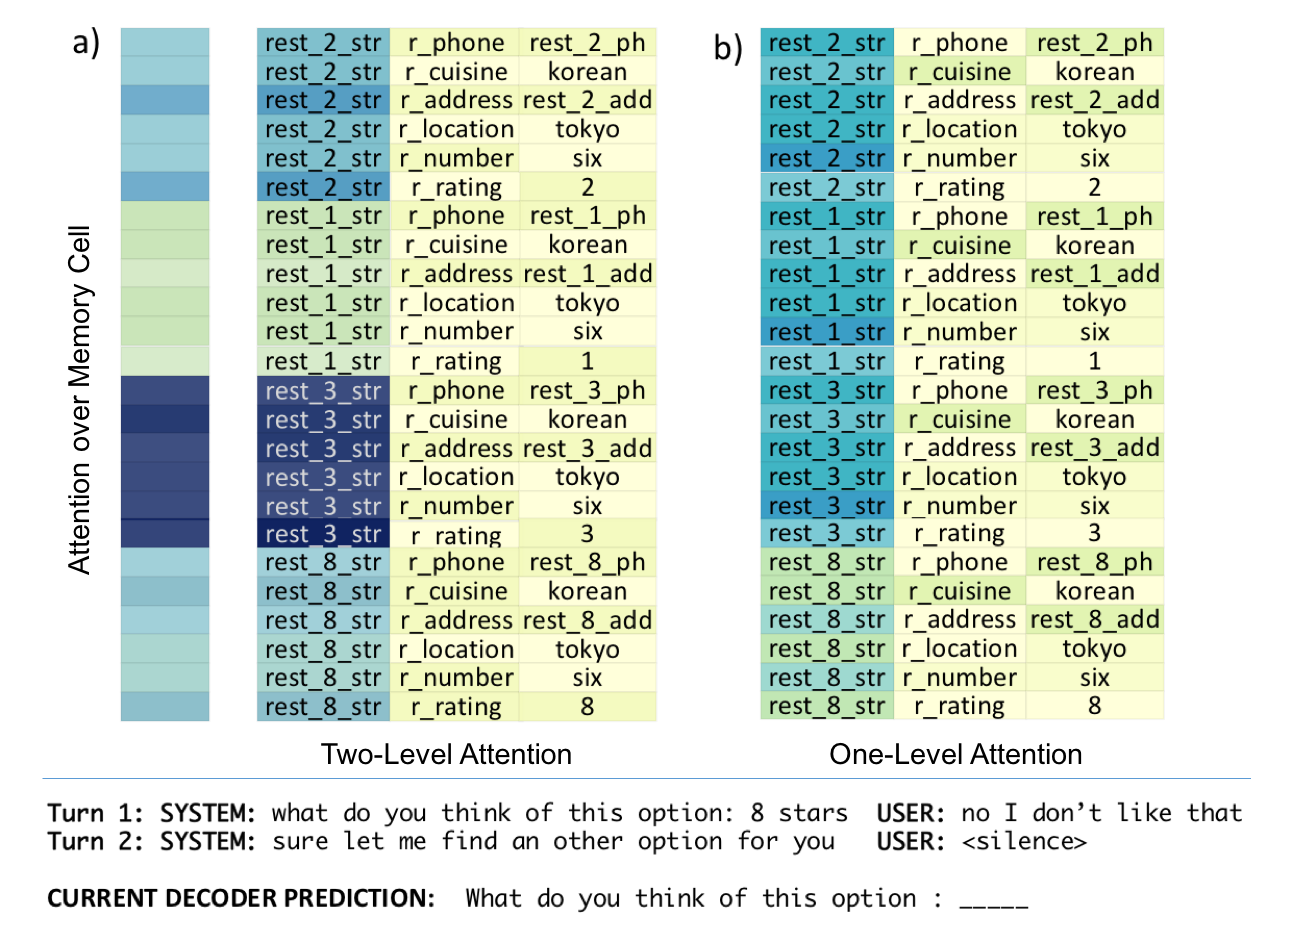
\includegraphics[width=\textwidth]{assets/task3_two_level.png}
\caption{Visualization of attention weights on selected portions of memory in (a) \sys\ with two-level attention vs (b) \sys\ with one-level attention}
\label{fig:attention}
\end{figure*}

\clearpage

\section{\sys -RL Experiments}

\subsection{Datasets}
We modified two of the previously used datasets: (1) \textbf{bAbI Task 3} and (2) \textbf{Camrest} and used them for this experiment. We removed the API call and the knowledge base results in both of the datsets and added a single {\em make API} symbol in their place.

\subsection{Baselines}
We used two baselines for this task

\noindent\textbf{Ground Truth} in which we provide the true API call for each dialog instance. It is more of a upper limit on the performance for the problem, rather than a baseline. 

\noindent\textbf{Greedy} in which we train the RL-decoder using supervised learning with the best APIs found during initial exploration as gold. We run exploration long enought to capture the highest reward APIs for each dialog, which is made feasible with our small search space.

\subsection{Results}
We train the RL-decoder using a two phase training mechanism. In the first phase we train just the RL-decoder till it nearly converges. In the second phase we start training the response encoder-decoder architecturee in tandem with the RL-decoder. 

During Phase 1 of the training, the decoder mangages to converge to 100\% perfect API prediction on the bAbI Task 3 train set in ~10 epochs. We show the performance on the corresponding test sets in Table \ref{tab:rl_res}. From the table we observe that the Ground Truth manages to reach nearly 84.5 percent accuracy. This is lower than the 94.6\% \footnote{This accuracy is caluculated by taking the responses of \sys\ on Task 3 and removing all the turns in which it had to predict an API call. Hence it doesn't match the reported 95.2\%} we achieved with \sys\ on the original Task 3 dataset. We attribute this difference to due hyperparameter tuning as we only had time for runs with one set of hyperparameters during the time of writing of this thesis.

Greedy mode is significantly lower in performance than the Ground Truth which can be attributed to data bias which plagues the greedy implementation. There is no provision for the greedy system to mitigate this bias as it only trains on APIs based on their reward. which might be equal for multiple APIs given our KB.

\sys\ -RL shows promising results on the first run and very closely matches the ground truth accuracies in both non-OOV and OOV test sets. This reflects on the ability of the system to successfully overcome the biases which effect MAPO with a normal decoder.

We do not report results on the Camrest dataset as they are still running during the time of writing of this thesis. Upto date infromation will be displayed in the README of the \sys -RL repository.

\begin{table}[t]
\centering
\footnotesize
 \begin{tabular}{l|c|c}
\toprule
& {\textbf{Task 3}} & {\textbf{Task 3 OOV}}  \\ 
\midrule
Ground Truth & \textbf{84.5} & \textbf{81.17} \\
Greedy & 74.9 & 74.28 \\
\midrule
\sys -RL & 82.98 & 79.41 \\
\bottomrule
\end{tabular}
\caption{\sys -RL Evaluation comparison with baselines on bAbI Task 3} 
\label{tab:rl_res}
\end{table}
\pagebreak

%%%%%%%%%%%%%%%%%%%%%%%%%%%%%%%%%%%%%%%%%%%%%%%%%%%%%%%%%%%%
% Appendices.

\appendix

\chapter{SUPPLEMENTARY}
\label{chap:appendix}
\section{Two-Level attention on BoSs Memory}
\label{ssec:hierarattn}

To visualize the benefit of two-level attention used on {\sc BoSs} memory by the decoder, we compare attention weights for two models: our proposed \emph{two-level attention} and a variant with just \emph{one-level attention} (over all the words in the memory). In the example of a sample dialog from bAbI Task 3, shown in Figure \ref{fig:attention}, the decoder is aimed at predicting the second best restaurant \textit{3 stars}, given that the restaurant with rating \textit{8 stars} has already been suggested and rejected. We show attention only on the KB entries for brevity.

The models share some similarities in their distribution of attention. First, the attention weights are localized over the restaurant names, indicating the preference of the system to point to a specific restaurant. This is supported by the $g_s$ values, $3.14$ x $10^{-5}$ and $1.15$ x $10^{-4}$ for two-level attention and one-level attention respectively, i.e., both models prefer to copy rather than generate. Moreover, entries with the same restaurant name have similar attention weights, reflecting the robustness of the distribution.

We also observe that two-level attention is able to perform the difficult task of {\em sorting} the restaurant entries based on decreasing order of rating (number of stars). It gives more weight to entries with a high rating 
(\textit{3 stars} $>$ \textit{2 stars} $>$ \textit{1 star})
and suppresses the weights of any previously suggested restaurant.
%, e.g., \textit{8 stars}. 

The attention over memory cells provides \sys\ with the ability to infer over multiple sets of tuples. The ability to sort the restaurants and reject a previously seen restaurant can be observed by the attention heat map of Memory cells. Attention over tokens on the other hand can push the attention weights towards either the subject or object in the KB tuple, based on the query's request. Thus using both in conjunction helps \sys\ perform significantly better than the baselines and illustrates the importance of the {\sc BoSs} memory in comparison to a flat memory layout.

\begin{figure*}
\centering
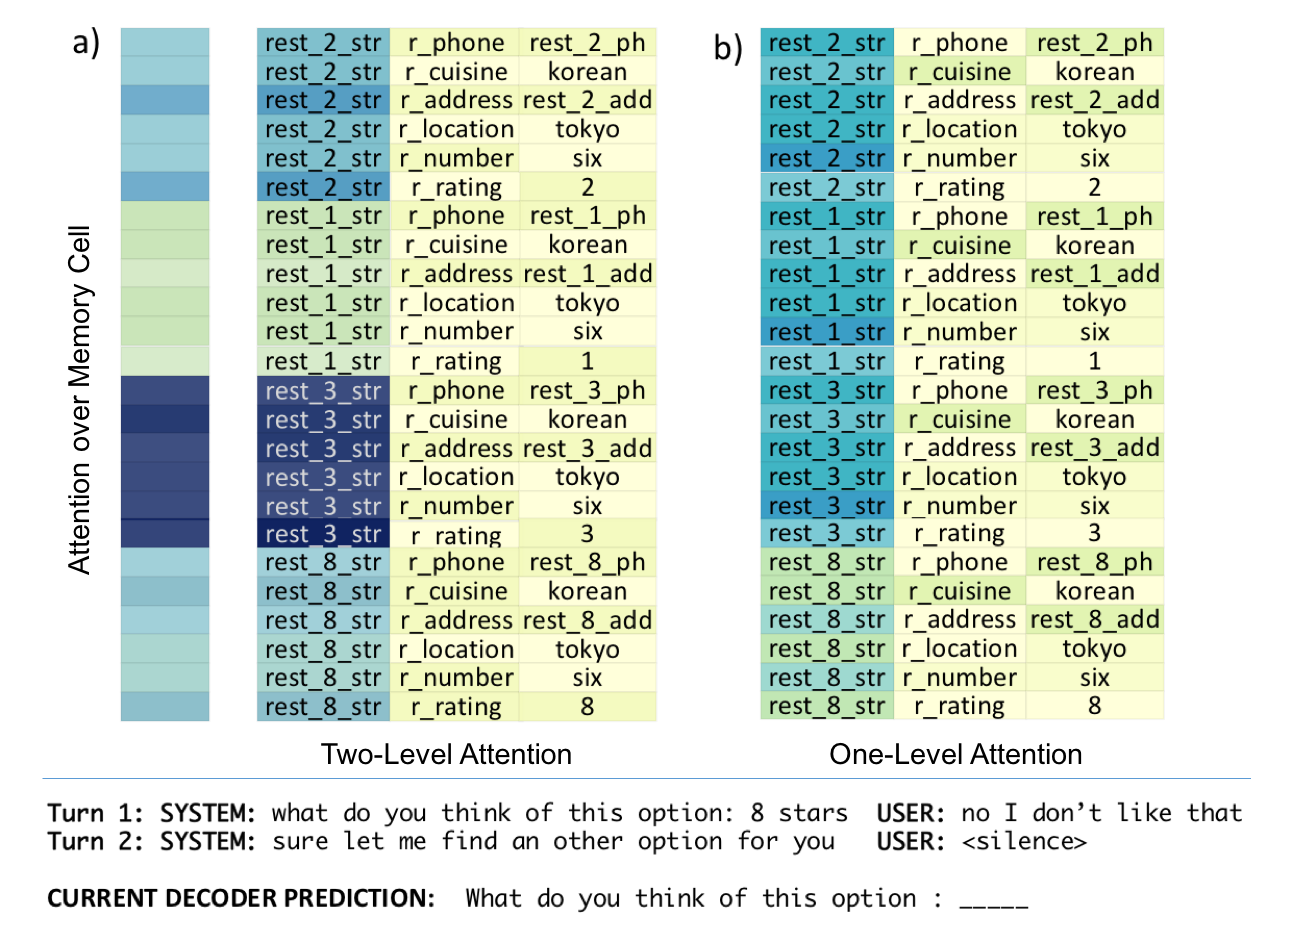
\includegraphics[width=0.8\textwidth]{assets/task3_two_level.png}
\caption{Visualization of attention weights on selected portions of memory in (a) \sys\ with two-level attention vs (b) \sys\ with one-level attention}
\label{fig:attention}
\end{figure*}

\section{Example Predictions of \sys\ and Baselines}
\label{sec:examples}
Examples from SMD is shown in Table \ref{tab:smd0} respectively. Examples from KA test set with percentage of unseen entites set to 50 from CamRest and SMD are shown in Table \ref{tab:cam50} and Table \ref{tab:smd50} respectively. Examples from KA test set with percentage of unseen entites set to 100 from bAbI dialog Task 1 is shown in Table \ref{tab:t1_100}.

\begin{table*}
\centering
\small
\begin{tabular}{c|l}

\toprule
% \multicolumn{2}{c}{\textbf{KB (restaurant|cuisine|address|phone|postcode)}} \\
% \multicolumn{2}{c}{\textit{prezzo}|\textit{ethiopian}|\textit{22\_seetharam\_nagar}|\textit{01799\_521260}|\textit{cb30ad}}\\
% \midrule
\midrule
\textbf{usr-1} &good morning \\
\textbf{sys-1} & hello what can i help you with today \\
\textbf{usr-2} & can you book a table with \textit{korean} cuisine for \textit{five} in \textit{beijing} \\
\textbf{sys-2} & i ' m on it . which price range are looking for ? \\
\textbf{usr-3} & i am looking for a \textit{overpriced} restaurant \\
\midrule
\textbf{Gold} & api\_call \textit{korean beijing five overpriced}
 \\
\midrule
\midrule
\specialcell[t]{\textbf{Seq2Seq+Copy}} & api\_call \textit{korean beijing five overpriced}
 \\
\midrule
\textbf{Seq2Seq} & api\_call \textit{french london four moderate} \\

\midrule
\textbf{Mem2Seq} & api\_call \textit{overpriced korean korean overpriced}
 \\
\midrule
\textbf{\sys\ } & api\_call \textit{korean beijing five overpriced} \\
\bottomrule
\end{tabular}
\caption{Example from bAbI dialog Task 1 with 100\% OOV.}
\label{tab:t1_100}
\end{table*}
\begin{table*}
\centering
\small
\begin{tabular}{c||p{13cm}}
\toprule
\multicolumn{2}{c}{\textbf{KB (restaurant|cuisine|address|phone|postcode)}} \\
\multicolumn{2}{c}{\textit{prezzo}|\textit{ethiopian}|\textit{22\_atlantis\_road}|\textit{01799\_521260}|\textit{cb30ad}}\\
\midrule
\midrule
\textbf{usr-1} &i want a \textit{moderately\_expensive ethiopian} restaurant in the \textit{south} side of town \\
\textbf{sys-1} & i ' m sorry . i can not find a \textit{moderately\_expensive ethiopian} restaurant in the \textit{south} side of town \\
\textbf{usr-2} & i would like to find a \textit{moderately} priced restaurant in the \textit{west} part of town \\
\textbf{sys-2} & \textit{prezzo} is a moderately priced \textit{ethiopian} restaurant in the \textit{west} part of town . there is also \textit{indian} and \textit{british} food available in that area and price range . would you like more info ? \\
\textbf{usr-3} & yes can i get thier address and postcode ? \\
\midrule
\textbf{Gold} & of course , \textit{prezzo} ' s address is \textit{22\_atlantis\_road} and postcode is \textit{cb30ad}
 \\
\midrule
\midrule
\specialcell[t]{\textbf{Seq2Seq+Copy}} & postcode a is is \textit{01223350688} UNK there get i for for today
 \\
\midrule
\textbf{Seq2Seq} & the address is \textit{83\_regent\_street} and their postcode is \textit{cb58aq} \\

\midrule
\textbf{Mem2Seq} & the phone address is \textit{cb21uj}
 \\
\midrule
\textbf{\sys\ } & the address is \textit{22\_atlantis\_road at 22\_atlantis\_road} the postcode is \textit{cb30ad} is there anything else i can help you with \\
\bottomrule
\end{tabular}
\caption{Example from Camrest with 50\% OOV. The OOV entities present in the dialog are \{\textit{ethiopian}, \textit{22\_atlantis\_road}\}}
\label{tab:cam50}
\end{table*}
\begin{table*}
\centering
\small
\begin{tabular}{c|p{13cm}}

\toprule
%\textbf{kb} & \textit{da\_vinci\_pizzeria}\\
% & \textit{r_phone|01223\_351707} \\
% & \textit{r_adddress|20\_milton\_road\_chesterton} \\
% & \textit{r_food|italian} \\
\multicolumn{2}{c}{\textbf{KB (location|distance|traffic info|address)}} \\
\multicolumn{2}{c}{\textit{teavana}|\textit{4\_miles}|\textit{no\_traffic}|\textit{145\_amherst\_st}}\\
\multicolumn{2}{c}{\textit{cafe\_venetia}|\textit{5\_miles}|\textit{moderate\_traffic}|\textit{269\_alger\_dr}}\\
\multicolumn{2}{c}{\textit{town\_and\_country}|\textit{3\_miles}|\textit{moderate\_traffic}|\textit{383\_university\_ave}}\\
\midrule
\midrule
\textbf{usr-1} & where can i get tea ? \\
\textbf{sys-1} & there is 2 tea shops near you \textit{teavana} is \textit{4\_miles} away and \textit{cafe\_venetia} is \textit{5\_miles} away which one do you want ? \\
\textbf{usr-2} & which one is the quickest is there any traffic ? \\
\midrule
\textbf{Gold} & \textit{teavana} is the fastest journey because there is \textit{no\_traffic} on the way there . \textit{cafe\_venetia} has \textit{moderate\_traffic} should we go to \textit{teavana}
 \\
\midrule
\midrule
\textbf{Seq2Seq+Copy} & there is
 \\
\midrule
\textbf{Seq2Seq} & there is \textit{moderate\_traffic} on the way to \textit{palo\_alto\_medical\_foundation} \\

\midrule
\textbf{Mem2Seq} & there is \textit{moderate\_traffic} on our way
 \\
\midrule
\textbf{\sys\ } & \textit{teavana} there is a \textit{moderate\_traffic} nearby but i might find another route to t\textit{own\_and\_country} \textit{town\_and\_country} address is \textit{383\_university\_ave} i sent it on your screen \\
\bottomrule
\end{tabular}
\caption{Example from SMD}
\label{tab:smd0}
\end{table*}

\begin{table*}
\centering
\small
\begin{tabular}{c|p{13cm}}

\toprule
\multicolumn{2}{c}{\textbf{KB (location|day|weather)}} \\
\multicolumn{2}{c}{\textit{mountain\_view}|\textit{sunday}|\textit{foggy}}\\
\multicolumn{2}{c}{\textit{mountain\_view}|\textit{monday}|\textit{overcast}}\\
\multicolumn{2}{c}{\textit{pittsburgh}|\textit{sunday}|\textit{overcast}}\\
\multicolumn{2}{c}{\textit{pittsburgh}|\textit{monday}|\textit{warm}}\\
\multicolumn{2}{c}{\textit{downtown\_chicago}|\textit{sunday}|\textit{foggy}}\\
\multicolumn{2}{c}{\textit{downtown\_chicago}|\textit{monday}|\textit{warm}}\\
\midrule
\multicolumn{2}{c}{\textit{today}|\textit{monday}}\\
\midrule
\midrule
\textbf{usr-1} &is the weather \textit{cloudy} right now ? \\
\textbf{sys-1} & what city do you want the weather for ? \\
\textbf{usr-2} & \textit{pittsburgh} \\
\midrule
\textbf{Gold} & there are no clouds in \textit{pittsburgh} right now
 \\
\midrule
\midrule
\textbf{Seq2Seq+Copy} & which is no
 \\
\midrule
\textbf{Seq2Seq} & it is currently raining in \textit{san\_francisco} right now \\

\midrule
\textbf{Mem2Seq} & it will not be cloudy in in
 \\
\midrule
\textbf{\sys\ } & it will be \textit{cloudy} on \textit{sunday} in \textit{pittsburgh} \\
\bottomrule 
\end{tabular}
\caption{Example from SMD with 50\% OOV. The OOV entity present in the dialog is \{\textit{pittsburgh}\}}
\label{tab:smd50}
\end{table*}

\section{Dataset Preprocessing and Faults}
\label{sec:preprocess}
\subsection{Mem2Seq Preprocessing}
\label{sec:prep_mem}

\begin{figure*}[ht]
\centering
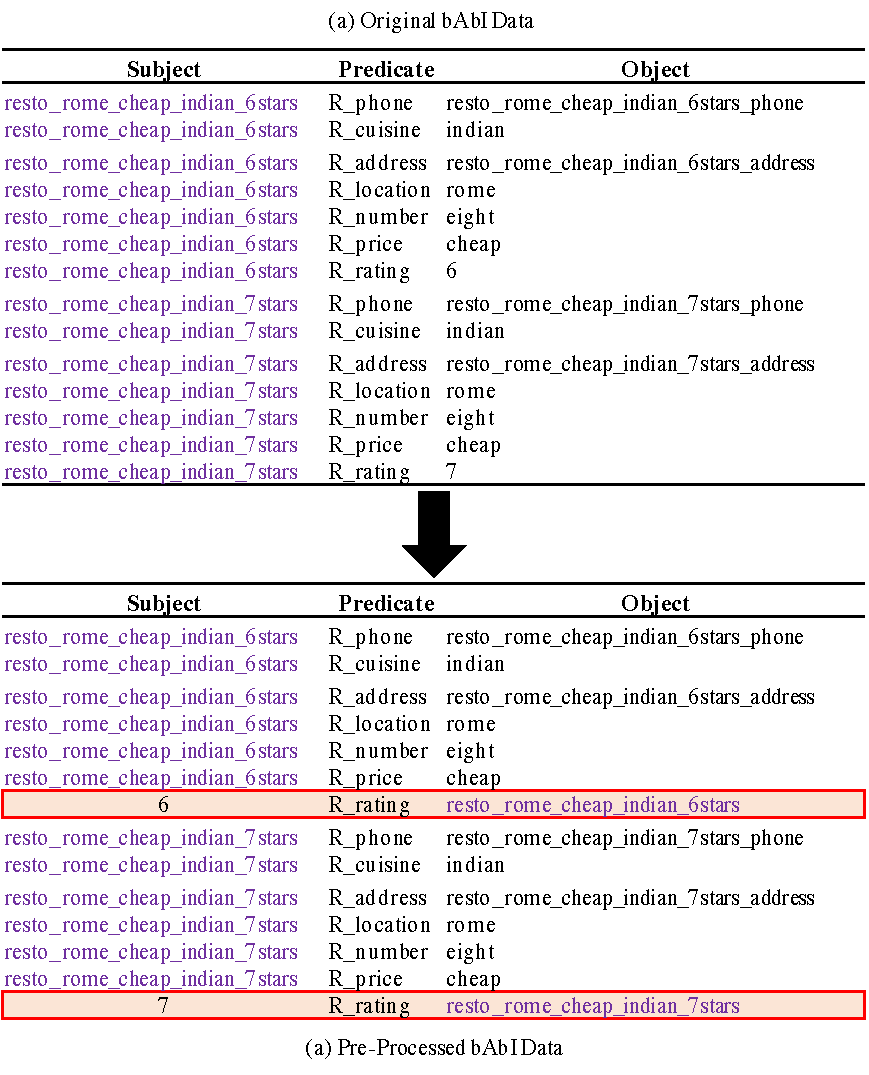
\includegraphics[width=0.8\textwidth]{assets/babi-preprocess.pdf}
\caption{Pre-processing of bAbI dialog data used in Mem2Seq paper}
\label{fig:prebabi}
\end{figure*}

\begin{figure*}[ht]
\centering
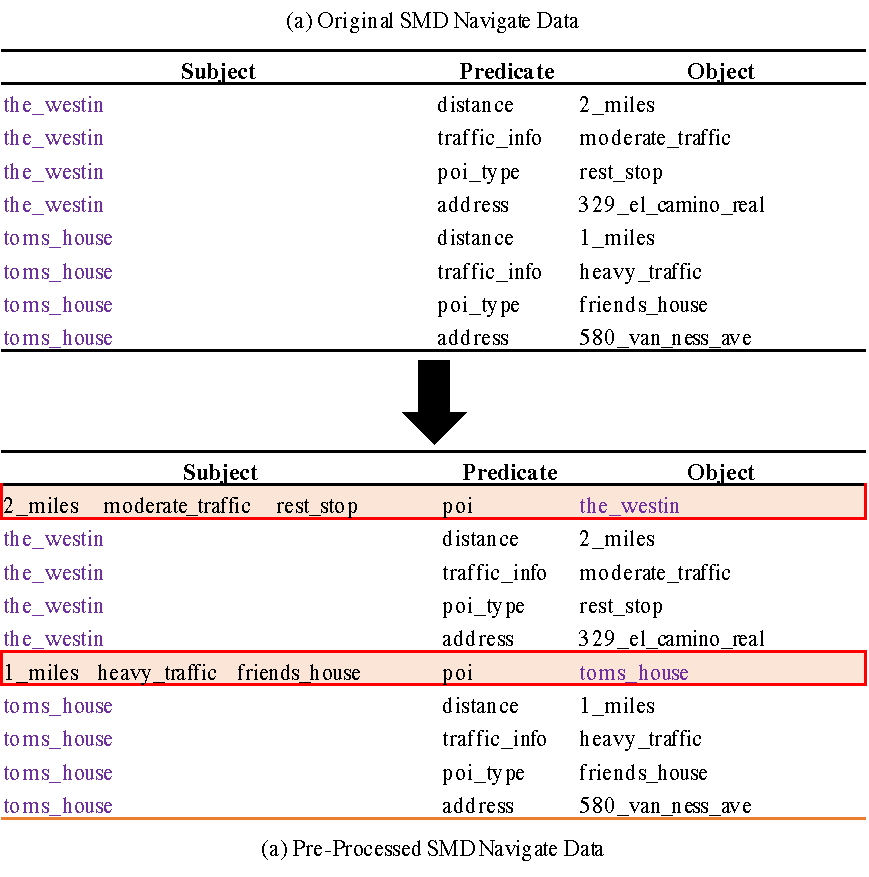
\includegraphics[width=0.8\textwidth]{assets/smd-preprocess.pdf}
\caption{Pre-processing of SMD Navigate data used in Mem2Seq paper}
\label{fig:presmd}
\end{figure*}

Mem2Seq paper used the following pre-processing on the data:
\begin{enumerate}
    \item The subject (restaurant name) and object (rating) positions of the rating KB tuples in bAbI dialogs are flipped, while the order remains the same for other tuples remains the same. This pre-processing is illustrated in Figure \ref{fig:prebabi}
    \item an extra fact was added to the navigation tasks in In-Car Assistant with all the properties (such as distance, address) combined together  as the subject and \textit{poi} as the object. This pre-processing is illustrated in Figure \ref{fig:presmd}
\end{enumerate}
The pre-processing has major impact on the performance of  Mem2Seq, as it can only copy objects of a KB tuple, while the subject and relation can never be copied.

\subsection{bAbI Dataset Faults}
\label{sec:fault}
The KB entities present in validation and non-OOV test sets for task 3 and 4 do not overlap with those in the train set. This effectively means that non-OOV and OOV test conditions are the same for tasks 3 and 4. This explains the low performance of baseline models on task 3 and 4 non-OOV test sets.

\section{Multi-Hop vs 1-Hop Encoders}
Table \ref{tab:ablationhop} shows the performance of bAbI tasks and CamRest on two \sys\ encoder settings. Multi-hops in encoder helps in bAbI task 3 and 5, as they require inferencing over the KB tuples (sorting restaurants by rating) to recommend a restaurant. We also see substantial improvements on CamRest in both BLEU and entity F1 metric.

\begin{table*}
\centering
\footnotesize
\begin{tabular}{l|ccccc|ccccc|cc}
\toprule
   & \multicolumn{5}{c|}{\textbf{bAbI Dialog Tasks}} & \multicolumn{5}{c|}{\textbf{bAbI Dialog Tasks (OOV)}}  & \multicolumn{2}{c}{\textbf{CamRest}} \\ \cmidrule{2-6} \cmidrule{7-11} \cmidrule{12-13}
    & T1  & T2  & T3   & T4   & T5   & T1 & T2 & T3 & T4 & T5 & BLEU        & Ent. F1       \\ \midrule
\sys\ with 1-Hop Encoder & 100 & 100 & 92.3 & 100 & 90.5 & 100 & 100 & 91.4 & 100 & 89 & 10.5 & 36.9 \\
\sys\ with Multi-Hop Encoder & 100 & 100 & 95.2 & 100  & 97.3 & 100    & 100    & 95.7   & 100    & 91.7   & 15.2        & 43.1    
\\ \bottomrule
\end{tabular}
\caption{Ablation study: impact of hops in \sys\ encoder }
\label{tab:ablationhop}
\end{table*}
\pagebreak

%%%%%%%%%%%%%%%%%%%%%%%%%%%%%%%%%%%%%%%%%%%%%%%%%%%%%%%%%%%%
% Bibliography.

\label{chap:references}
\bibliography{survey}
\addcontentsline{toc}{chapter}{REFERENCES}
\pagebreak

%%%%%%%%%%%%%%%%%%%%%%%%%%%%%%%%%%%%%%%%%%%%%%%%%%%%%%%%%%%%
% List of papers

\listofpapers
\begin{enumerate}
\item Yavuz et Al.  \newblock
{\bf DEEPCOPY: Grounded Response Generation with Hierarchical Pointer Networks}
  \newblock {\em NIPS} (2018).

\item Ebrahimi et Al.  \newblock
{\bf Reasoning over RDF Knowledge Bases using Deep Learning}
  \newblock {\em arXiv} (2018).

\item Singh et Al.  \newblock
 {\bf Towards VQA Models That Can Read}
  \newblock {\em CVPR} (2019).

\item Golchha et Al.  \newblock
 {\bf Courteously Yours: Inducing courteous behavior in Customer Care responses using Reinforced Pointer Generator Network}
  \newblock {\em NAACL-HLT} (2019).

\end{enumerate}

\end{document}
